%%% Local Variables:
%%% TeX-master: "master"
%%% End:

\documentclass[10pt]{report}
% \usepackage[margin=1in]{geometry}
% \newcommand\hmmax{0}
% \newcommand\bmmax{0}
% % % Fonts% %
\usepackage{luatexja}

\usepackage[T1]{fontenc}
   % \usepackage{textcomp}
   % \usepackage{newtxtext}
   % \renewcommand\rmdefault{Pym} %\usepackage{mathptmx} %\usepackage{times}
\usepackage[complete, subscriptcorrection, slantedGreek, mtpfrak, mtpbb, mtpcal]{mtpro2}
   \usepackage{bm}% Access to bold math symbols
   % \usepackage[onlytext]{MinionPro}
   \usepackage[no-math]{fontspec}
   \defaultfontfeatures{Ligatures=TeX,Numbers={Proportional}}
   \newfontfeature{Microtype}{protrusion=default;expansion=default;}
   \setmainfont[Ligatures=TeX,BoldFont={*-Semibold}]{Source Serif Pro}
   \setsansfont[Microtype,Scale=MatchLowercase,Ligatures=TeX,BoldFont={*-Semibold}]{Source Sans Pro}
   \setmonofont[Scale=0.8]{Atlas Typewriter}
   % \usepackage{selnolig}% For suppressing certain typographic ligatures automatically
% % % % % % %
\usepackage{amsthm}         % (in part) For the defined environments
\usepackage{mathtools}      % Improves  on amsmaths/mtpro2
\usepackage{xfrac}

% % % The bibliography % % %
\usepackage[backend=biber,
  style=authoryear-comp,
  bibstyle=authoryear,
  citestyle=authoryear-comp,
  uniquename=false,
  % allinit,
  % giveninits=true,
  backref=false,
  hyperref=true,
  url=false,
  isbn=false,
  useprefix=true,
  ]{biblatex}
\DeclareFieldFormat{postnote}{#1}
\DeclareFieldFormat{multipostnote}{#1}
% \setlength\bibitemsep{1.5\itemsep}
\newcommand{\noopsort}[1]{}
\addbibresource{Ability.bib}
% % % % % % % % % % % % % % %

\usepackage[inline]{enumitem}
\setlist[enumerate]{noitemsep}
\setlist[description]{style=unboxed,leftmargin=\parindent,labelindent=\parindent,font=\normalfont\space}
\setlist[itemize]{noitemsep}

% % % Misc packages % % %
\usepackage{setspace}
% \usepackage{refcheck} % Can be used for checking references
% \usepackage{lineno}   % For line numbers
% \usepackage{hyphenat} % For \hyp{} hyphenation command, and general hyphenation stuff

% % % % % % % % % % % % %

% % % Red Math % % %
\usepackage[usenames, dvipsnames]{xcolor}
% \usepackage{everysel}
% \EverySelectfont{\color{black}}
% \everymath{\color{red}}
% \everydisplay{\color{black}}
\definecolor{fuchsia}{HTML}{FE4164}%Neon Fuchsia %{F535AA}%Neon Pink
% % % % % % % % % %

\usepackage[export]{adjustbox}
\usepackage{subcaption}

% \usepackage{pifont}
% \newcommand{\hand}{\ding{43}}
\usepackage{array}

\usepackage{multirow}
% \usepackage{adjustbox}

\usepackage{multicol}

\setcounter{secnumdepth}{4}
\setcounter{tocdepth}{4}

\usepackage{tikz}
\usetikzlibrary{bending,arrows,positioning,calc,arrows.meta,patterns,fadings}
\usetikzlibrary{trees}
\usepackage{tikz-qtree} %for simple tree syntax
% \usetikzlibrary{positioning,shapes.multipart} %for structured nodes
\usetikzlibrary{tikzmark}

\usepackage{graphicx} % for images (png/jpeg etc.)
\usepackage{caption} % for \caption* command

\usepackage{tabularx}

% \usepackage{svg}
% \usepackage[off]{svg-extract}
% \svgsetup{clean=true}

\usepackage{dashrule}

\newcommand{\hozline}[0]{%
  \noindent\hdashrule[0.5ex][c]{\textwidth}{.1pt}{}
  %\vspace{-10pt}
  % \noindent\rule{\textwidth}{.1pt}
}

% \usepackage{pdfrender}
\usepackage{extarrows}

% % % My commands % % %

\newcommand{\hozlinedash}[0]{%
  \noindent\hdashrule[0.5ex][c]{\textwidth}{.1pt}{2.5pt}
  %\vspace{-10pt}
}
% % % % % % % % % % % %

\usepackage{xskak} % For chess diagram

% % % My packages % % %
\usepackage{CustomTheorems}
% \usepackage{FuturePromisedEvents}
\usepackage{ThesisCustom}
\usepackage{Notes}
% % % % % % % % % % % %

\usepackage[hidelinks,breaklinks]{hyperref}
\usepackage[]{bookmark}

\title{
  Ability to reason and reasoning with ability \\
  \large Outline
}
\author{Ben Sparkes}
% \date{ }

\begin{document}

% \newpage

\maketitle

\tableofcontents

\part{Overview}

%%% Local Variables:
%%% TeX-master: "master"
%%% End:

\chapter{Overview}
\label{cha:overview}

\section{Outline}
\label{sec:outline}

\begin{note}
  In this chapter we provide a high level overview of the main arguments made in this thesis.
  A significant part of the high level overview of arguments is an overview of the premises and assumptions that those arguments rest on.

  By given high level overview, clarify on how premises, assumptions, and conclusions relate.
  In the main body of the thesis, afford to elaborate.
  And, allow choice of where to seek elaboration.
\end{note}

\begin{itemize}
\item Start with claiming support, used throughout, so important.
\item Introduce and motivate plausible constraint on support, to be argued against/exception for.
\item Outline exception.
\item High level overview of argument for exception.
\item Major and minor.
\item Largely fairly high level sketch of major argument.
\item Type of ability information.
\item Understanding \emph{de re} ability reading.
\item \AR{} and \WR{}.
\item For the moment, brief, much more detail in relevant chapter.
\item Relation between \AR{} and \uRa{}.
\item Constraint on reading of ability.
\item Requires argument for \WR{}.
\item Introduce \nI{}.
\item Sketch argument for \nI{}.
\item Link \nI{} and \AR{}.
\item Completes overview of major argument.
\end{itemize}

\section{Ability and access to claimed support}
\label{sec:abil-access-supp}

\begin{note}
  Following introduction, interest is with ability.
  In particular, observation that \gsi{} information, and confidence in general ability seems to allow agent to claim support for result.

  Question on what basis the agent claims support.

  Slightly more general statement.
  \begin{quote}
    When and why an agent may claim support for the result of reasoning that the agent has not witnessed.
  \end{quote}
  Ability claims of interest provide some answer to `when'.
  For, ability provides information about what the result is, and also that the agent has the opportunity to perform the reasoning.\nolinebreak
  \footnote{No claim to necessity}

  Suggested in introduction, answer to `why' is more complex.
  % \begin{quote}
  %   Our interest is in when an agent may claim support for some conclusion of some instance of reasoning on the basis of the support the agent may claim for the premises of the instances of reasoning.
  % \end{quote}
\end{note}

\begin{note}[Introducing support]
  Initial clarification is with respect to claiming support.
  Emphasis on `\emph{claim}'.

  The thesis is not about when and why an agent \emph{has} support for the result of reasoning that the agent has not witnessed.

  Two reasons for this.
  First, neutral for main thread of argument on what support amounts to.
  Interest is with structure of claim, and background assumption that if success in claiming then structure of support follows structure of claim.

  Second, whether or not an agent has support often seems secondary.
  To illustrate:
  It may be that any claimed support for a proposition is support for that proposition, but perhaps not.
  Suppose `flan' is written on the side of a container.
  I may claim support that the container contains flan.
  And, it may be that the writing on the side of the container is support for the box containing flan.
  However, the straps ensuring the container remains closed is unfortunately placed, and if moved would reveal the side of the container reads `flannels'.
  The unfortunate placing of the straps does not seem to prevent \emph{claiming} support, but I'm not sure whether it is right to say that the writing on the side of the box (straps in place) \emph{does} the box containing flan.
  So, in what follows I will speak in terms of claiming support, and leave open whether what is claimed reflects on whether an agent has support.\nolinebreak
  \footnote{
    In particular, claiming allows focus on internal constrains, while remaining silent on whether having support is (in part) determined by external factors.
  }
  \(^{,}\)\nolinebreak
  \footnote{
    Distinction between propositional and doxastic support.
    Propositional, support agent has whether or not made a claim.
    Doxastic is successful claim and propositional support.
    So, both require that the agent has support.
    Claimed support is the agentive component of doxastic support.
    Not interested in whether the agent also has propositional support, though more or less assume.
  }
  \(^{,}\)\nolinebreak
  \footnote{
    {
      \color{red}
      English is somewhat difficult.
      It is somewhat unfortunate that `an agent has claimed support for \(\phi\)' may be read `there is support which the agent has claimed for \(\phi\)'.
      Still, this seems to follow more easily from `support claimed'.
      So, `claimed support' emphasises the claim, while `support claimed' emphasises support.
    }
  }
\end{note}

\subsection{Background for claiming support and reasoning}
\label{sec:claimed-support}

\begin{note}[Understanding of claiming support]
  Understanding of claiming support.

  Begin with a sufficient condition.
  In short, most instances of reasoning.
  Claiming support is common.

  Then, two types of defeaters.
  Mistaken and misled.
  Use to form a necessary condition.
  If claimed support, then agent deems that claimed support is not defeated.
  `Deem' is a placeholder.
  Strong or weak.
  Single constraint is that when claiming support, potential defeaters that aren't ruled out.\nolinebreak
  \footnote{
    At least two ways of viewing this.
    First, claiming support is restricted.
    Second, \emph{claiming} support only applies when there are potential defeaters, and some other relation to support when possible defeaters get ruled out.

    These are different, but I don't think the difference matter for resource bound agents of interest.
    Lack of resources is that always potential defeater, even if every possible defeater may be ruled out.
    }
  Finally, property, that claimed support does not depend on whether proposition the agent has claimed support for is true, or whether the claimed support \emph{does} support (if these are separated).
  Property will be important.
\end{note}

\begin{note}[Sufficient condition]
  We start with a sufficient condition for claiming support:
  \begin{proposition}[\bP{-} --- \bP{}]\label{prem:bP}
    If an agent may claim support for premises and steps of reasoning, accesses those premises and traces claim to support through those steps of reasoning, then agent may claim support for conclusion on basis of the claimed support for the steps and premises of reasoning.
    (Given that the agent deems that the claims to support for premises and steps used are undefeated when drawing conclusion.)
  \end{proposition}

  The purpose of taking~\bP{} as basic is to fix a basic understanding of when an agent may claim support.
  In short, an agent may claim support when reasoning goes well.
  And, reasoning goes well when there are premises and steps of reasoning available to the agent, and the agent draws on these to claim support for the conclusion.
  The parenthetical remark is a simple safeguard, the agent does not lose a claim to support for the premises or steps in the process of reasoning.\nolinebreak
  \footnote{
    May think that this is the wrong safeguard.
    Consider the liar paradox:
    `This sentence is false.'
    \bP{} prevents agent from claiming support that the sentence is true or false.
    However, may think that agent is in a position to claim support that the sentence is both true and false.
    Indeed, standard reasoning associated with the liar suggests that the sentence is both true and false.
    Still, it's not obvious from demonstrating that the sentence is both true and false that one may claim support for the sentence being true and the sentence being false.
    That is, one may confine the paradox to the truth value of the sentence, rather than (associated) surplus of support.
  }
  We consider defeaters below.
  First, an illustration.


  Suppose an agent measures that the box in front of them has the dimensions of \(19\text{cm}\) by \(7\text{cm}\).
  The agent understands how to calculate the area of a box, and by performing some reasoning comes to hold that the area of the box is \(133\text{cm}^{2}\).
  The support the agent has for holding that the area of the box is \(133\text{cm}^{2}\) is obtained (at least in part) on the measurement of box, understanding how to calculate the area of box, and some grasp of arithmetic.

  Whether some (or all) of the required arithmetic is to be included as a premise or a step of reasoning may be set aside.
  Similarly, set aside whether further arguments, or whether some premises and steps are taken as basic.
  For example, perhaps some the agent requires some further claim to support for using the ruler to measure the box such as comparison to a standard, or perhaps the agent's claim to support terminates by noting that their use of the ruler is a reliable process.
\end{note}

\begin{note}[Value proposition]
  Reasoning and claims to support focus.
  Briefly introduce a pair of propositions to clarify claim to support and reasoning.

  \begin{proposition}[Claimed support is for the value of a proposition]\label{prop:csifvoap}
    When an agent claims support for some proposition, the agent claims that the proposition has some value.
    Where:
    \begin{itemize}
    \item A proposition is some state of affairs. And,
    \item A value is an assessment of a state of affairs.
    \end{itemize}
  \end{proposition}
  The role of \autoref{prop:csifvoap} is primarily to fix terminology.
  To illustrate, when stating the conclusion of the reasoning sketched above we used the proposition that \emph{the area of the box is \(133\text{cm}^{2}\)}.
  The proposition refers to the state of affairs in which the area of the box is \(133\text{cm}^{2}\), and speaking a little more precisely, the agent claimed that the proposition has the value `true' --- though it may be the value turns out to be `false'.
  Or, perhaps if the agent was a little unsure about the accuracy of the ruler, that the proposition has the value `likely', `probable', or some quantitative credence.
  And, some other instance of reasoning may have concluded that the proposition has the value `desirable' --- e.g.\ if the agent was searching for a box of some approximate size.\nolinebreak
  \footnote{
    Nothing in particular hangs on the distinction between different values.
    If you prefer, you may expand the proposition (state of affairs) to include additional factors, and consider only the values `true' and `false'.
    For example, the proposition that \emph{I desire the bath to be warm} is false, as opposed to the proposition that \emph{the bath is warm} is valued undesirable by me.
  }

  Core idea is that claim of support is that things are a certain way.
  Proposition, what the thing is.
  Value, the way it is.
  In most cases the value will be clear (i.e. that the proposition is true, though sometimes that the proposition is desirable), and so we will talk of claiming support for the proposition.
  A handful of additional examples will be provided when illustrating the next proposition.
\end{note}

\begin{note}[Reasoning proposition]
  \begin{proposition}[Reasoning as establishing value]\label{prop:RisTV}
    Reasoning, tracing value through propositions/establishing that proposition has value.
  \end{proposition}

  \begin{itemize}
  \item Testimony, so claim support that \emph{p} is true.
  \item Unreliable, so claim support that \emph{p} improbable.
  \item Religious text, so claim support that \emph{p} ought to be the case.
  \item Producer, so claim support that album is desirable.
  \end{itemize}

  In a deductive case, if the premises are true, then the conclusion is true.
  Means-end reasoning for desire.
  The value is important.
  If it is true that it past 6pm, then it is true the shop is closed.
  Provides value of shop being closed.

  However, if agent desires that it is past 6pm, then it doesn't follow that the agent desires that the shop is closed.
  Question an agent as to why they think their desires conform to truth --- is-ought problem.

  Means-end reasoning.
  It is true that there is cheese at the centre of the maze.
  And, it is desirable that I obtain the cheese at the centre of the maze.
  Further, it is true that I may only obtain the cheese at the centre of the maze by solving the maze.
  Therefore, it is desirable that I solve the maze.
\end{note}

\begin{note}[Moving to value]
  \color{red}
  Important to note is that way in which agent claims support is important.

  Preface paradox.
  Here, move to value, but these are isolated.
  Don't get to combine these together, no allowed to hold that these are simultaneously true.
  Or, simultaneously assign value to the individual propositions.

  So, move isn't free, so to speak.
\end{note}

\begin{note}
  \begin{proposition}[Defeaters for claimed support]
    There are at least two ways in which a claim to support may be defeated.
    \begin{itemize}
    \item Claimed support may (discovered to be) be \emph{misled} by suggesting that a proposition has some value that it does not (in fact) have. And,
    \item Claimed support may (discovered to be) be \emph{mistaken} by appealing to factors that do not indicate the value of the proposition.
    \end{itemize}
  \end{proposition}
  Misleading support may indicate value, and value may have value indicated by mistaken support.
  Both are defeaters in the sense that, were the agent to learn that the claim to support was misleading or mistaken, then the agent would not hold that the proposition has the value indicated by the (problematic) claim to support or the basis of that (problematic) claim to support.

  Common to distinguish between countervailing and undercutting defeaters.
  Countervailing, support for some other proposition.
  Undercutting, force of claimed support is mitigated.

  Both misled and mistaken are instances of being undercut.
  For, if mistaken or misled then the support is no good.

  Neither are clearly cases of countervailing.
  For, no relation to other support is required.
  However, presence of countervailing implies misled.
  Countervailing does not imply mistaken, though may in some cases demonstrate so.

  Below suggest that when claiming support the agent excepts that claimed support is not misleading or mistaken.
  Hence, given that countervailing implies misled, implicitly take claimed support for a proposition to indicate absence.
  (This is another purpose from separation from support.)

  ???
\end{note}

\begin{note}[M\&M Illustration]
  To illustrate:

  Suppose I glance at the clock on the wall.
  The clock reads 11:45a, so I claim support that it is 11:45a.
  However, it may be the case that the clock is incorrectly set, and the time is 11:15a, or 12:15p, etc.\
  By claiming support from the time expressed by the clock, I would have been \emph{misled} about what the time actually is.
  For, it is not true that the time is 11:45a.
  Though, in all other respects, there may be no fault with claiming that the time is as expressed by the clock and so the claim to support is not mistaken.

  By contrast, suppose I glace at the clock on the wall.
  The clock reads 11:45a, so I claim support that it is 11:45a.
  By claiming support from the time expressed by the clock, I would have been \emph{mistaken} about what the time actually is.
  For, the time expressed by a broken clock is not a good indicator of what the time actually is.
  Though, despite the clock being broken, it is 11:45a and so the claim to support is not misleading.

  And, claimed support for the time from a broken clock expressing the wrong time would be both misled \emph{and} mistaken.\nolinebreak
  \footnote{
    A second illustration:
    Consider a smoke detector, designed to sound an alarm if and only if sufficient levels of smoke are detected.
    Hence, if the alarm sounds, one may claim support there being smoke in the room where the alarm is installed.
    One may be misled; the alarm may have malfunctioned, so no fire.
    Or, one may be mistaken; the same type of alarm may be installed in a different room, wouldn't be a useful indicator.
  }
\end{note}

\begin{note}[Subjectively sound]
  Of course, clocks are typically glanced at, and a glance at a clock is often insufficient to determine whether the clock is incorrectly set or broken.
  Hence, the \emph{possibility} that a clock is incorrectly set or broken --- or more broadly the possibility that claimed support is misleading or mistaken --- does not prevent an agent from claiming support.
  So, ensuring that to-be-claimed support would be neither mistaken or misleading is not a necessary condition for claiming support.
  Rather, we endorse the following condition with respect to these types of defeaters:

  \begin{proposition}[Adequacy of claimed support]\label{prop:CSNMORM}
    If agent claims support for some proposition, then
    % from the perspective of the agent,
    the agent deems that the claimed support
    % adequate whether or not the claimed support may (in fact) be
    is not misleading nor mistaken --- the agent has some expectation that possible defeaters (of the two types of noted) do not obtain.\nolinebreak
    \footnote{
      Stronger than distinct claim that the agent does not deem that the claimed support is misleading or mistaken.
      Stronger requires, presence of some deeming.
      Later does not.
    }
  \end{proposition}
  If some expectation that they do, then this seems enough to deny support.
  If no attention to defeaters, questionable whether any claimed support.

  If the claimed support is not misleading, then the proposition has the value the claimed support indicates the proposition has.
  And, if the claimed support is not mistaken, then the claimed support indicates the value.
\end{note}

\begin{note}[Agents are fallible]
  The missing piece of \autoref{prop:CSNMORM} is an account of what `deem' amounts to.
  The following proposition (\ref{prop:fallibility}) states an assumption, which allows a (general) functional characterisation of `deem'.

  \begin{proposition}[Agents are fallible]\label{prop:fallibility}
    When claiming support for a proposition and agent is never in a position to rule out the (epistemic) possibility that the claimed support is not misled or mistaken.
  \end{proposition}

  I take it to be intuitive that agents are fallible in many cases of claiming support.
  It is not too difficult to think of ways in which claimed support may be misleading or mistaken.
  As noted above, claiming support for what the time is from glancing at a clock seems sufficient, but clocks may be incorrectly set (misled) or broken (mistake).
  Similarly, a sample of \(1,000\) rolls may mislead me into thinking that a die is unbiased, or an overloaded operator may lead to a mistake in claiming support for the proposition that \(x = 4\) is an expression of equality rather than variable assignment.

  \autoref{prop:fallibility} states that an agent is never in a position to rule out the possibility that the claimed support is not misled or mistaken.
  This does not entail that there are defeaters, nor that there are any possible defeaters --- only that defeaters are an epistemic possibility.

  Still, in some cases, this may seem absurd.
  Suppose in front of me are two apples and two pears.
  So, four pieces of fruit.

  However, those appears and pears may not be real pieces of fruit, they may be replicas.
  So beings the process of attempting to quarantine fallibility from infallibility.

  There are two pairs of objects in front of me, and the objects appear to be fruit.
  So, there are four objects in front of me, which appear to be fruit.

  There are two pairs of objects hence there are four objects.

  But I may be hallucinating.

  There appear to be two pairs of objects in front of me, which appear to be fruit.
  So, there appear to be four objects in front of me, which appear to be fruit.

  Whenever there are two pairs of objects, there are four objects.

  Even so, I'm not in a position to rule out the possibility that arithmetic is inconsistent.

  Perhaps identity is a stronger candidate: Any object is identical with itself --- but I doubt one needs to claim support for reflexivity of equality.
  Similarly, it doesn't seem to be the case that I need to claim support for the proposition that my name is ミスタ --- no matter what my birth certificate says, I get to decide what my name is.

  Rather than fix a specific account of the `possibility' modal used, here are a handful compatible interpretations:

  \begin{enumerate}[label=\Alph*., ref=(\Alph*)]
  \item\label{CS:I:Never} \emph{In principle} it is not possible for any agent to rule out the possibility that claimed support is not misleading or mistaken.
  \item\label{CS:I:Resources} It is not possible for a \emph{resource bound agent} to rule out the possibility that claimed support is not misleading or mistaken.
  \item\label{CS:I:Class} There is a restricted class of propositions for which and agent is required to claim support, and it is not possible for any agent to rule out the possibility that claimed support for a proposition belonging the class is not misleading or mistaken.
  \end{enumerate}

  To illustrate, consider the proposition that there is an external world:
  \ref{CS:I:Never} denies that there could be, e.g.\ proof of an external world.
  \ref{CS:I:Resources} denies that agents of interest could not demonstrate such a proof even if it were to exist.
  \ref{CS:I:Class} allows an agent may not be required to claim support for the existence of an external world.

  I expect the intended application of claimed support will be compatible with each interpretation, and specifically with respect to \ref{CS:I:Class}, that the propositions will belong to the highlighted class.\nolinebreak
  \footnote{
    I favour the combination of \ref{CS:I:Resources} and \ref{CS:I:Class}, and to leave open whether an idealised agent may rule out the possibility of being misled or mistaken with respect to some propositions when claiming support.
  }\(^{,}\)\nolinebreak
  \footnote{
    In particular, true of ability.
  }
\end{note}

\begin{note}
  Given some interpretation of the possibility modal, the functional role of `deem' is to provide resistance to possible defeaters that an agent is not in a position to rule out.
  How resistant the agent's claimed support needs to be is up to you.

  Provide a test below to help with intuition.
  Before doing so, final proposition, which follows as a corollary from previous.
\end{note}

\begin{note}[\eiS{}]
  Subjectively sound, claimed support indicates value.

  Final proposition.
  Definition.

  \begin{definition}[Dependence and independence]
    An agent's claimed support for \(\phi\) \emph{depends} on some value of \(\psi\) just in case the agent would not claim support for \(\phi\) given any other value of \(\psi\).

    An agent's claimed support for \(\phi\) is \emph{independent} of \(\psi\) just in case the agent's claimed support does not depend on the value of \(\psi\).
  \end{definition}

  Claiming support is independent of value.

  \begin{proposition}[\eiS{-} --- \eiS{}]\label{prop:supp:independence}
    If agent claims support for some proposition, \(\phi\), then the claimed support is taken to indicate the value of \(\phi\) independently of the value of \(\phi\) or whether the claimed support is `genuine' support.
    Equivalently, the claimed support is taken to indicate the value of \(\phi\) does not require that the claimed support is not misled or mistaken.\nolinebreak
    \footnote{
      Possibly goes against externalism, but I don't think this is right.
      External circumstances may impact the support the agent has.
      However, as these are external, it seems this condition plausibly holds for \emph{claiming} support.
      This is how you get puzzles for externalism.
      In both cases, it's fine for the agent to claim support, but the external circumstances impact whether the agent \emph{has} support.
      The internalist/externalist divide would seem to affect the conditions on claiming.

      Way to expand on this is reconstructing bootstrapping examples with and without \eiS{}.
      If the agent would only get basic support if reliable, then it's not clear that bootstrapping is a problem.
    }\(^{,}\)\nolinebreak
    \footnote{
      One way independence.
      Not clear that value is independent of support.
      So long as sufficiently strong support, not possible for proposition to have value other than claimed support.
    }
  \end{proposition}
  \eiS{} follows from Propositions~\ref{prop:CSNMORM} and~\ref{prop:fallibility}.

  From Proposition~\ref{prop:CSNMORM}, deemed that claimed support is neither mistaken nor misled.
  From Proposition~\ref{prop:fallibility}, always possibility.

  Suppose depends on value of \(\phi\).
  Still, from Proposition~\ref{prop:fallibility}, (epistemic) possibility that value of \(\phi\) differs.
  If differs, then claim to support is misleading.
  By Proposition~\ref{prop:CSNMORM} agent deems not mistaken or misled, and so deems that possible defeaters do not obtain.
  However, requirement of \(\phi\) denies the relevant possibility.
  For, if different value of \(\phi\) then no claim to support.
  Therefore, agent does not deem the claimed support not misleading.


  For, possibility that \(\phi\) does not have value, or that claimed support does not indicate.
  And, given claim to support requires that the possibility does not obtain, agent has not deemed that the claimed support is not misled or mistaken --- rather the agent requires that the claimed support is not misled or mistaken.

  \eiS{} does not deny that things may need to be a certain way for an agent to claim, or to be in a position to, claim support.
  It may be the case that no agent would be in a position to claim support that the speed of light is constant if the speed of light were not constant, but in claiming support an agent must deem that possible defeaters do not obtain, e.g.\ that the laws of nature are constant, and that no mistakes have been made when observing relevant phenomena.

  The force of the corollary is that agent does not require \(\phi\) related things being a certain way in order to claim support for \(\phi\).

  See with failures of `even if\dots' test.
\end{note}

\begin{note}[Quick clarification on \eiS{}]
  A quick clarification may be in order.

  \eiS{} is only about value/support for\(\phi\).
  So, \eiS{} does not prevent agent from claiming support for \(\psi\) from value of \(\xi\) given claimed support that \(\xi\) has that value.
  For example, an agent may claim support that \emph{p} is true from claimed support that \emph{S} knows \emph{p}.
  And, the agent may do so because the proposition that \emph{S} knows \emph{p} is true only if \emph{p} is true.
  That is, so long as the agent does not require \emph{p} to be true in order to claim support for the proposition that \emph{S} knows \emph{p} is true.
  We will return to \eiS{}, expand on this quick clarification, and note related observations in Section~\ref{sec:second-conditional}.
\end{note}


\begin{note}[Adequate reasoning]
  Term this \emph{adequate} reasoning.
  May be good, may involve mistakes, may be bad.
  Kind of reasoning that we, the folk, do.
  Distinction for claiming support is that this is different from whether the agent has support, and we may set issues about whether the agent has support.

  Our interest is what is required for an agent to \emph{claim} support for (premises and) steps of reasoning, rather than what is required for an agent to \emph{have} support for (premises and) steps of reasoning.

  Use support as opposed to justification.
  Initial focus is on epistemic/doxastic attitudes.
  However, practical reasoning.
  For example, means-end.
  Support considered quite general to also include this.
\end{note}




\begin{note}
  To help fix intuition, I suggest a (hypothetical) test to clarify what is meant by `deem': The `even if\dots' test.
  So long as an agent may provide an adequate responses to the test, the agent will be in a position to claim support.
\end{note}

\begin{note}[The `Even if\dots' test]
  The `Even if\dots' test queries whether an agent's claimed support permits an agent to expect that some (epistemically) possible defeater fails to obtain `even if' it does obtain.

  For example, even if \(0.999\dots = 1\), there must be \emph{some} difference between \(0.999\dots\) and \(1\) --- no matter how small --- and some difference between to things is sufficient to establish that they are not equal.

  Implied in this response is something like the observation that \(0.9 = (1 - 0.1)\) and \(0.99 = (1 - 0.01)\), and so \(0.999\dots = (1 - 0.000\dots 1)\), hence \(1 = (0.999\dots + 0.000\dots 1)\), and because \(0.999\dots\) refers to some quantity, \(0.000\dots 1\) likewise refers to some quantity.
  It seems reasonable for an agent to expect that the Archimedean property does not hold for real numbers.

  The example given is an instance of the applied to the possibility that the agent's claimed support that \(0.999\dots \ne 1\) may be misleading, as the antecedent supposes that \(0.999\dots = 1\).

  Generalising, we have outlined two kinds of defeaters that would prevent an agent from claiming support.
  The two types of defeaters suggest two basic instances of the test:
  \begin{enumerate}
  \item[(ML)] Even if \(\phi\) does not have value my claimed support indicates, I deem it to be the case that\dots
  \item[(MT)] Even if I some part (or whole) of my claimed support for the value of \(\phi\) is mistaken, I deem it to be the case that\dots
  \end{enumerate}
  Below we provide three examples for each basic instance of the test, two (plausibly) successful responses and one (plausibly) unsuccessful response..\nolinebreak
  \footnote{
    You may think that some of the adequate responses I suggest are too weak, but for future purposes I require only that some positive answer many be given, and so you may strengthen the requirements on a positive answer as you see fit.
  }
\end{note}

\begin{note}[Even if: misled]

  We being with two plausibly satisfactory responses to being misled.

  \begin{enumerate}[label=(ML\arabic*), ref=(ML\arabic*), series=ML_counter]
  \item\label{ML:asleep} Even if that person is not sleeping, their eyes have been closed for a long time and their breathing is slow.
  \item\label{ML:lying} Even if you are telling the truth, the scientific consensus is against you.
  \end{enumerate}

  With \ref{ML:asleep} the agent has claimed support for the proposition that the person is sleeping.
  It's not too hard to give the impression of being asleep, so there is some possibility that the person is awake and support claimed is misleading.
  Still, even if the person is awake, the person is exhibiting sufficient signs of being asleep for the agent to expect that they are not misled.

  Turning to \ref{ML:lying}, it may be that the person is telling the truth and if the person is indeed telling the truth then any claimed support for a conflicting proposition must be mistaken.
  However, scientific consensus seems sufficient to claim support for the relevant conflicting proposition --- one expects that scientific consensus is not misleading given the rigours of the scientific process.
  Scientific consensus does not (at least typically) require that the person is not telling the truth (though will imply that to be the case).

  In contrast, consider an unsatisfactory response.

  \begin{enumerate}[label=(ML\arabic*), ref=(ML\arabic*), resume*=ML_counter]
  \item\label{ML:forgery} Even if this certificate is a forgery, it professes to be the real thing.
  \end{enumerate}
  If the certificate is a forgery, then the claimed support for the proposition that the certificate is not a forgery would be misleading.

  The response to the (epistemic) possibility that the certificate is a forgery is unsatisfactory because the agent depends on the certificate not being a forgery.
  Hence, that the certificate self-certifies it's authenticity is no response to the (possibility) that it is a forgery.
  Immediate conflict with \eiS{}, and traces back to \autoref{prop:CSNMORM} because it seems quite unreasonable to expect that the certificate is not a forgery based on it's self-certification.

  Of course, many certificates do self-certify (it would be excessive effort to identify a certificate and then be required to find information about what the certificate is for), and perhaps a simple observation that there are no signs of tampering may be a sufficient response to the `even if\dots' test.
\end{note}

\begin{note}[Even if: mistaken]
  Turning to the possibility of mistaken support, consider the following two instances of the `even if\dots' test.

  \begin{enumerate}[label=(MT\arabic*), ref=(MT\arabic*), series=MT_counter]
  \item\label{MT:fake-wound} Even if that is a fake wound, I have no way to tell and the actions of the (apparently) wounded would be a feat of acting.
  \item\label{MT:misquote} Even if the newspaper has quoted the wrong person, the paper has a strong record of accurate reporting.
  \end{enumerate}

  With respect to~\ref{MT:fake-wound}, it seems a mistake to treat a fake wound as indicate the presence of an actual wound, as a fake wound does not require a genuine would but likewise a fake wound may cover a genuine wound.
  The response to the `Even if\dots' test notes that the behaviour of the (apparently) wounded person is sufficiently consistent with their expectations of the behaviour of a person with the (apparent) wound, and would lead to be surprised if the person was not in fact wounded.

  Turning to~\ref{MT:misquote}, if the paper has quoted the wrong person then it would be a mistake to claim support that the person said whatever-it-is-they-said, though it may still be the case that the person did say whatever-it-is-they-said.
  Even so, the strong record of the paper seems sufficient for the agent to expect that the newspaper has not misattributed or imagined the quote on the relevant occasion.

  In contrast, consider an unsatisfactory response.

  \begin{enumerate}[label=(MT\arabic*), ref=(MT\arabic*), resume*=MT_counter]
  \item Even if this library does not using LCC indexing, the library does not have a copy of `Measurement Theory' because as search for `H61 .R593' returns no results.
  \end{enumerate}
  Holding that a library does not have a copy of a book because a search for the book under a particular indexing system would be a mistake.
  For, if the library does not use the particular indexing system then a search using that indexing system will always fail, regardless of whether or not the library has a copy of the book.

  In turn, a failed search for an LCC index in the library's database does not seems sufficient for an agent to claim that the library does not have a copy of the book unless the agent is in a position to claim support that the library uses LCC indexing.
  Following, it seems the failed response to the `Even if\dots' test may be supplemented by noting that the library is a research library, and therefore likely uses LCC indexing, etc.\
\end{note}

\begin{note}[Even if: more]
  Primary observation from these examples is that in positive cases provided responses indicate that some response to possibility of being misled or mistaken is available to the agent.
  In the failure cases, no response.

  % Cases of entailment, preface paradox.
  % Mistake somewhere.
  % Here, support is good for each of the claims made in the preface, but these do not combine to make a case that no mistake has been made across any of the claims.
  % May come down to familiar concerns, too significant possibility of being misled.
  % May also think that claimed support for each might require a mistake in one.
  % I.e. source for claim includes further claims which state that source for some other claim is mistaken.
  % Problem with using both sources, even if for distinct propositions.

  % Interesting problem later.
  % For now, simple example.
  An interesting case for misled is the preface paradox.
  Claimed support for everything in the preface, but also claimed support for mistake.
  Credence resolves tension, remains noteworthy that even if confident of some potential defeater, claimed support is sufficient to resist undermining claimed support.

\end{note}

\begin{note}[???]
  \color{red}
  Possible defeaters, so no claim that the reasoning is sound.
  However, agent deems that no defeaters, so may term this `\emph{subjectively} sound' reasoning.

  At least two worries.
  First, given general use of the term `support', considerations may suggest iterated support.
  Second, worries about over-intellectualisation of claiming support.
\end{note}


\begin{note}[Closing support]
  To summarise, claim of support.
  Certain kind of independence.
  Only interested in support, and not how this relates to attitudes.
  Somewhat intuitive, but no claims that this is the only understanding of support.

  For the moment, this provides clarity for understanding of support.
  Below, use to argue for failure to claim support.
\end{note}

\subsection{Interest with claiming support and reasoning}
\label{sec:inter-with-claim}

\begin{note}[Focus]
  We will argue against the converse of~\bP{}:

  \begin{proposition}[\uRa{-} --- \uRa{}]\label{denied-claim}
    An agent may claim support for some conclusion of reasoning by claiming that the conclusion of reasoning is supported by premises and steps of reasoning \emph{only if} the agent has witnessed the reasoning (i.e.\ traced the claimed support for those premises and steps used to claim support for the conclusion).\nolinebreak
      \footnote{
    Three brief notes on~\uRa{}:

    First, the `has' in~\uRa{} only requires `at some point in the past'.
    Hence,~\uRa{} does not require the agent to reason from premises to conclusion each time the agent claims support for the conclusion.
    For example, if an agent proved the Deduction Theorem for propositional logic last week, then the agent would not be in conflict with~\uRa{} if they claimed support for the Deduction Theorem on the basis of the premises and reasoning they performed in the past.

    Second, and following from the first,~\uRa{} will also hold for any stronger statement --- for example if `has' is read as `has just'.
    For example, requiring that the agent's memory of proving the Deduction Theorem allows the agent to claim support, rather than the premises and steps used in the past.
    The argument (stated below) denies that, given certain information, the agent needs witnesses any reasoning in order to claim support for the result of witnessing the reasoning.

    Third, as~\uRa{} is about when an agent may \emph{claim} support, it is compatible with~\uRa{} to hold that the agent \emph{has} support --- regardless of whether the agent has witnessing the reasoning.
  }
  \end{proposition}

  \uRa{}, as the converse of~\bP{} focuses on reasoning, and our focus will be with~\uRa{} because our interest is with reasoning.
  However, the key claims of~\uRa{} are independent of reasoning.
  To clarify,~\GuRa{} is a generalisation of~\uRa{}.

  \begin{proposition}[\GuRa{}]
    An agent may claim support for some proposition \emph{p} by appealing to some materia\nolinebreak
    \footnote{Latin.
      Material, matter, basis, information, foundation, ground, etc.
    }
    \emph{M} only if the agent has used \emph{M} to claim support for proposition \emph{p}.
  \end{proposition}
  Our focus is with whether an agent is required to have \emph{used} something in order to appeal to that thing when claiming support.
  No fixed understanding of `use' is assumed in the statement of~\uRa{} and~\GuRa{}, and we will offer some disambiguation below.
  First, a basic illustration.
\end{note}

\begin{note}[Illustration]
  To illustrate~\uRa{}, consider the illustration provided for~\bP{}.

    If the agent did not measure the box, understand how to calculate the area of a box, or perform the arithmetic, the agent would not be in a position to claim support that area of the box is \(133\text{cm}^{2}\).
  A lucky guess that the area of the box is \(133\text{cm}^{2}\) would not allow the agent to hold that the area of the box is  \(133\text{cm}^{2}\) on the basis of the dimensions of the box, the agent's understanding of how to calculate the area of a box, and arithmetic.
  And, it seems the agent is not in a position to base their lucky guess in such a way because the agent did not reason from the dimensions of the box, the agent's understanding of how to calculate the area of a box, and arithmetic.\nolinebreak
  \footnote{
    Moving to another agent, observe doing the work, get report.
    Easy to resist, by adding in additional premise.
    Still, no presupposing that this needs to be done.
  }
  Similarly, if an agent learns that a box with dimensions of \(19\text{cm}\) by \(7\text{cm}\) may be calculated to have an area of \(133\text{cm}^{2}\), then the agent may not claim support for the area of the box on the basis of the calculation.
  If the agent has not performed the calculation, then the agent may not appeal to the use of the calculation when claiming support --- rather, the agent mentions that the calculation is true.\nolinebreak
  \footnote{
    Slight weakening of~\uRa{} may be made.
    So long as \emph{some} agent has performed the calculation.
    Argue against~\uRa{}, and the argument made will hold for this weakening.
  }
\end{note}

\begin{note}[Intuition]
  \uRa{} and~\GuRa{} seems quite plausible, at least to me.
  The proposition is a careful statement of an intuitive ideas:

  Whether or not an agent claims support is the result of the structure of the reasoning process, and if some premises or step is not used, then it is irrelevant to the structure of the process.
  Hence, the only premises and steps of interest when claiming support are those used in the reasoning process.

  Rests on the broader idea from~\GuRa{}.
  Claiming support is the result of some agentive process, and the result of an agentive process is explained by the constituents of the process.\nolinebreak
  \footnote{
    Ah, the homonculus.

    Question about whether the agent is important.

    This gets difficult.

    Consider clocks.
    Clock does not keep track of time.
    Rather, mechanical system designed to change in constant with some passage of time. (Cf.\ \textcite{Smith:1988aa.}.)

    Agent may be like this.
    Distinction is intentionality.
    When I go about keeping track of the time, I'm attempting (at least typically) to maintain reference to what the time is.
    Figure out a way to approximate a second, and that's what's happening.
    Approximation.
    If it is noted that I requarly sigh every minute, use this, but I wouldn't be keep tracking of time, though you may be using regularity to do so.
    So, in the former case, using understanding of time, while in the latter not doing so.
  }

  As~\GuRa{} is restricted to an agent claiming support, things seem a little easier.
  Problems with interpretation, however.
  Transparency.
  Familiar, if debatable, illustration.
  Freud.
  (Here, adjourning the meeting by saying something mistaken.)
\end{note}

\begin{note}[Analogy]
  By analogy, whether or not my mug of (once cold) coffee overheats in the microwave is the result of some process involving electromagnetic radiation.
  My desire that the mug of coffee does not overheat is not used as part of the process of heating the coffee, and so is irrelevant to the structure of the process.

  My desire may explain why the mug of coffee is taking part in a certain process, and an unused premise or step may explain why an agent performed so reasoning.
  Still, a premise or step must be used as part of the process of reasoning to stand in explanation for the result of reasoning.

  Press the analogy further: Reasoning is a causal process.
  And, any property of reasoning reduces to cause and effect.
  If premises or steps are not used, then those premises or steps stands outside the relevant causal trace, and may not be appealed to when accounting for some structural property of the conclusion of the instance of reasoning (here, that the agent claims support for the conclusion).
\end{note}

\begin{note}[Causal theories of basing]
  Indeed,~\uRa{} seems to be implied by causal theories of basing.
  Consider \citeauthor{Moser:1989tv}'s account of the basing relation:
  \begin{quote}
    \emph{S}'s believing or assenting to \emph{P} is based on his justifying propositional reason \emph{Q} \(=_{\text{df}}\) \emph{S}'s believing or assenting to \emph{P} is causally sustained in a nondeviant manner by his believing or assenting to \emph{Q}, and by his associating \emph{P} and \emph{Q}.\nolinebreak
    \mbox{}\hfill\mbox{(\cite*[157]{Moser:1989tv})}
  \end{quote}
  Believing or assenting is plausibly general enough to encompass claiming support for \emph{P},\nolinebreak
  \footnote{
    Recall, intuitive explanation of claiming support is whatever it is that happens with doxastic justification.
  }
  and \emph{Q} may stand for premises and steps of reasoning.
  \citeauthor{Moser:1989tv}'s definition is with relation to propositional reason \emph{Q}, which may be understood as support (in contrast to \emph{claimed} support).
  Still, this is defined in terms of believing or assenting to \emph{Q}, i.e.\ claiming support for \emph{Q}, and a causal relation between \emph{P} and \emph{Q}.

  The causal requirement distinguishes \citeauthor{Moser:1989tv}'s account of the basis relation.
  However, our focus was on the relation to \emph{Q}.
  So, may expect that the observation extends to other accounts of the basing relation.\nolinebreak
  \footnote{
    \color{red}
    Need some quick mentions here.
  }
\end{note}

\begin{note}[\uRa{} does not imply CTB]
  Important, however, is that \uRa{} does not imply any causal theory of basing.
  For, \uRa{} does not imply any theory of basing.
  Rather, \uRa{} is about when an agent may claim support, and does not touch on how the support is based.
\end{note}

\begin{note}[Segue]
  Causal, use as having some effect.
  Contrast, understand use for intentionality.
\end{note}

\begin{note}[Moving on from basing]
  Still, as basing relation is epistemic, it may be useful to observe a further example, even if structurally similar.
\end{note}

\begin{note}[Representationalism]
  \citeauthor{Neta:2019aa} generalises (purely) epistemic interest in basing relations to cover the explanatory relation between reasons and (rationally evaluable) states held, or actions performed, by an agent.

  On the way to a novel proposal, \citeauthor{Neta:2019aa} sketches a broad characterisation of representationalist theories of (generalised) basing:
  \begin{quote}
    (R1\('\)) for an agent to C based on reason R involves not merely the agent's representing R as justifying C---it also involves this latter representation (or its content) being part of the reason why the agent C's.\nolinebreak
    \mbox{}\hfill\mbox{(\citeyear[197]{Neta:2019aa})}
  \end{quote}

  To illustrate, claim support that [some number] is prime.
  It's possible that I did the prime factorisation, and possible that I took that representation to be part of the reason why I claim that [XXX] is prime.
  However, represented query of whether prime to wolfram alpha as justifying, and that's why I claimed support.

  Broadly stated, representationalist and causal accounts of the basing relation are compatible.
  Still, the relation between representationalist accounts and~\uRa{} may be more visible.
  For, a representationalist account would require (minimally) that an agent represents premises and steps of reasoning as justifying when claiming support for some conclusion of reasoning, which suggests use of those premises and steps.
  The implied use may be weaker than an intuitive reading of `use' --- it is not clear that representing an entailment is the same as reasoning with an entailment --- but it seems plain to me that representing some reason as justifying is a use of that reason.\nolinebreak
  \footnote{
    Alternatively, a clause may be added to~\uRa{} which denies that the agent represents the relevant premises and steps of reasoning.
    The argument made against~\uRa{} is compatible with the use of representations, or mere representation even if unused --- though it is unclear to me what an unused but represented premise or step would matter when claiming support.
  }
\end{note}

\begin{note}[Responding to reasons]
  As final motivation, consider the proposal at the core of \citeauthor{Lord:2018aa}'s (\citeyear{Lord:2018aa}) thesis that being rational is to correctly respond to reasons.

  \begin{quote}
    \textbf{Correctly Responding:} What it is for A's \(\phi\)-ing to be ex post rational is for A to possess sufficient reason S to \(\phi\) and for A's \(\phi\)-ing to be a manifestation of knowledge about how to use S as sufficient reason to \(\phi\).\nolinebreak
    \mbox{}\hfill\mbox{(\citeyear[143]{Lord:2018aa})}
  \end{quote}

  An agent's action is rational only if the action is a manifestation of some know-how.
  \citeauthor{Lord:2018aa} summaries:

  \begin{quote}
    \dots when one manifests one's know-how, dispositions that are directly sensitive to normative facts are manifesting. Thus, the competences involved in the relevant know-how make one directly sensitive to the normative facts\nolinebreak
    \mbox{}\hfill\mbox{(\citeyear[16]{Lord:2018aa})}
  \end{quote}

  For our purposes, following example of manifesting know-how directly relates to reasoning:

  \begin{quote}
    The most salient disposition [when appealing to \emph{p} as a reason]\nolinebreak
    \footnote{Note, \citeauthor{Lord:2018aa} (explicitly) not talking about believing that \emph{p} is a reason, but argues that the cited disposition to present both when appealing to p as a reason and believing that \emph{p} is a reason.}
    is the disposition to (competently) use \emph{p} as a premise in reasoning.\nolinebreak
    \mbox{}\hfill\mbox{(\citeyear[25]{Lord:2018aa})}
  \end{quote}

  Hence, suppose an agent appeals to a premise of reasoning in order to claim support for some conclusion.
  Then, if the agent does not use the premise of reasoning, it seems the agent does not manifest know-how, which is required for the appeal to meet \citeauthor{Lord:2018aa}'s account of rational action.

  Of course, that the noted disposition is the most salient does not rule out alternative, less noteworthy, dispositions.
  However, it is unclear to me how to \emph{manifest} know-how without use.
  Looking ahead, it does not seem to be the case that I manifest my ability to show that a certain rule of inference is sound when skipping over details in a completeness proof.
  However, I may manifest know-how regarding the (presumed) truth of the ability attribution.

  Likewise with my ability to establish a preference for tofu over any other kind of miso when ordering soup.
\end{note}

\begin{note}[Summarising illustrations]
  Three examples of claiming or establishing relations of support have been given.
  Each example suggests that if an agent does not use a premises or steps when claiming support, then an agent may not claim support by appeal to the unused premises or steps.

  Stepping back,~\uRa{} may be seen as a desiderata for any account of (successfully) claiming support.
  For:
  If an agent (successfully) claims support for some conclusion of reasoning, then that claim of support is the result of some reasoning.
  The relevant reasoning that culminated with the claim to support involved some premises and steps of reasoning.
  So, given that the agent appealed to certain premises and steps when claiming support for conclusion, some property of the premises and steps an adequate account of claiming support must explain how the premises and steps used permit the agent to claim support.\nolinebreak
  \footnote{
    Note, however, that this argument does not imply that support for the conclusion must be accounted for in terms of the premises and steps used by the agent to claim support.
    For example, one may hold that an enthymematic argument permits an agent to claim support, while the relevant relation of support is secured by the corresponding non-enthymematic argument.
    Cf.\ \textcite{Moretti:2019wx} for suggestions along these lines.
  }
\end{note}

\begin{note}[Where \uRa{} is okay]
  I think~\uRa{} and~\GuRa{} are fine from an aetiological perspective --- account for how or why it came to be that the agent claimed support --- but question whether this restricts what the agent appeals to.
\end{note}

\begin{note}[Alternative]
  \uRa{} is a universal claim, and so applies to all instances in which an agent may claim support for conclusion on basis of support for premises and steps of reasoning --- an agent may only claim support if the agent reasoned from the premises via the steps to the conclusion.

  Our goal is to motivate an exception to \uRa{}:
  \begin{proposition}[\rC{-} --- \rC{}]\label{rC}
    If an agent has claimed support that they have the ability to (adequately) reason to some conclusion, then the agent may claim support for the conclusion by claiming support for the premises and steps of reasoning that the agent would use when witnessing their ability to reason to the conclusion.
  \end{proposition}

    The exception is motivated by the agent having information that they have the ability to (adequately) reason to the conclusion.
  Key is that if~\rC{} is true, then the agent is not required to use having the ability to reason as a premise.
  Instead, the agent may instead appeal to the premises (and steps) that would be used when witnessing the ability.

  Loosely restated,~\rC{} holds that if an agent may claim support for having the ability to witness some reasoning, and is aware of the conclusion of that reasoning, then the way in which the agent claims support for the conclusion of that reasoning may mirror the way in which the agent would claim support for the conclusion by witnessing the reasoning (and hence using the relevant premises and steps).

  So, if~\rC{} is true, then there are cases in which an agent is not required to reason from premises they may claim support for to some conclusion in order to obtain support for the conclusion on the basis the support the agent has for the premises.\nolinebreak
  \footnote{
    Stated~\rC{} as an exception to~\uRa{}.
    And, we will argue that~\rC{} is true.
    However, we will not argue that~\rC{} \emph{is an exception} to~\uRa{}.
    To do so would require an argument that \uRa{} holds for other cases.
    Likewise, no argument that~\rC{} is the only exception, as to do so would require argument that~\uRa{} holds for all other cases.
  Take~\uRa{} to be plausible, and suspect that there are few, if any, further exceptions, but~\rC{} may stand independently on any further statements about claiming support.
  }

  The alternative, in line with~\uRa{}, would be for the agent to use the proposition that they have the ability.

  To illustrate.
  Inform me that I have the ability to demonstrate that the area of a box with dimensions \(19\text{cm}\) by \(7\text{cm}\) has area \(133\text{cm}^{2}\), then so long as long as I get to claim support for having the ability.
  However, \emph{that I have the ability to demonstrate that the box has the certain area} and \emph{that the box has a certain area} are distinct propositions.
  \rC{}, when I claim for \emph{that the box has a certain area}, I appeal to dimensions and formula, though as I do not witness the ability, I do not use the premise and step.

  This is by no means obvious.
  A plausible view is that there is an entailment form the proposition \emph{that I have the ability to demonstrate that the box has the certain area} to \emph{that the box has a certain area}, and (in line with \uRa{}) I use the entailment.

  Indeed, I think that such reasoning is permissible in many cases.
  \rC{} permits exceptions to \uRa{}, but it does not require all instances of reasoning with ability is an exception to \uRa{}.
  The primary argument for \rC{} is that \uRa{}, certain instances of reasoning with information about ability, and a principle concerning when an agent is permitted to claim support are in tension.

  Specifically:
  Information that one has some specific ability so long as one has some general ability --- such as the (specific) ability to show that \(25^{\circ}\text{C} = 77^{\circ}\text{F}\) given the (general) ability to convert between Celsius and Fahrenheit.
  And, agent is never permitted to claim support for proposition if require value in order to claim support.
  The details matters, and we postpone detailing this argument to section~\ref{sec:broad-argum-overv}.
\end{note}

\begin{note}[Segue]
  For now, we close the present section with a handful of remarks concerning ability and~\rC{}.
\end{note}

\begin{note}[Ability]
  Idealised agents have no need to appeal to ability.
  However, for limited agents, ability is abundant, while the resources required to witness abilities are scarce.
  That the exception to~\uRa{} is narrow does not entail that there are few occurrences of the exception.

  Information about ability may be abundant while the resources for witnessing abilities are either scarce or temporarily unavailable.
  So, for example, agent has the option of conserving or deferring use of resources.

  If~\rC{} then a novel perspective on limited agents.
  When and why limited agent may claim support for result of reasoning.
  Here, conflict with appeal to~\uRa{} it its unrestricted form.

  And, in between propositional and doxastic support (or more commonly justification).
  Propositional support doesn't allow agent to claim support.
  Doxastic support, agent does claim support.
  If ability allows agent to claim support, \dots

  Secondary motivation is with ability to reason itself.
  Even if arguments for~\rC{} fail to convince, not much has been said on ability to reason, and first steps are useful.

  Third, use of~\uRa{}.
  Potential alternative conclusions to arguments that appeal to~\uRa{} as a premise.
  Revise premises for arguments in which~\uRa{} is a conclusion.
  As an exception, even if~\rC{}, conclusion of arguments which appeal to or assume \uRa{} may be restricted.
\end{note}

\begin{note}[Actual support]
  As with~\uRa{}, \rC{} does not entail that the agent \emph{has} support.
  Doesn't show that the agent has support.
  {
    \color{red}
    Some more notes on why this is important.
    Basically, this means that~\rC{} isn't too strong.
  }
  Still, it take it to be plausible that support traces a successful claim.
  From this perspective,~\rC{} may seem a little more intuitive.
  Given an intuitive understanding of support, if an agent does have the ability to reason to some conclusion, then the conclusion stands in the relation of being support by certain premises and steps of reasoning, whether or not the agent witnesses their ability.
  In turn, if the agent may claim support for the having the relevant ability then the agent may claim support for the conclusion from the premises and steps that would be used when witnessing their ability because witnessing would not contribute to the relation of support between the conclusion and the relevant premises and steps --- witnessing would only clarify to the agent the specifics of the relation.

  Of course, agent may be mistaken or misled about having ability, and witnessing may be expected to highlight.
  The combination of relevant premises and steps may fail to establish the conclusion, or be out of reach of the agent.
  However, consequences of the possibility of mistaken or misled regarding having the ability.
  Not clearly any worse than being mistaken or misled and using that one has the ability as a premise, which in turn seems no different to the possibility of being mistaken or misled about any arbitrary premise.
\end{note}

\begin{note}[Examples]
  Need quick truth and desire examples.
  I don't think I need to make these examples compelling, as giving borderline examples may help motivate interest.

  Claimed support is general, extends to desires.\nolinebreak
  \footnote{
    Strong view on which an agent may be mistaken about desires in the same way as an agent may be mistaken about evidence.
    View on which desires are independent of representation.
    Hence, misleading or mistaken support when an agent fails to represent desire.
  }
  Here, temptation.
  Ability to demonstrate that abstaining from a \(\text{n}^{\text{th}}\) glass of wine, even though the reasoning the agent performs after the \(\text{n-1}^{\text{th}}\) glass supports drinking another glass.

  There are alternatives.
  One follows motivation of \uRa{} as a desiderata.
  Agent abstains, and so some part of the reasoning involved sufficiently strong desire to abstain.
  Or, appeal to an intention, blocking out relevance of a (stronger) desire to drink the \(\text{n}^{\text{th}}\) glass of wine and to allow action to follow from the (weaker) desire to abstain.
  Or, desire to do what your are confident you are able to establish as the result of reasoning about the thing to do.

  Still, proposal in line with~\rC{} is of some interest.
  Weakness of will (in some cases) as reluctance to expend resources.
  So, true that strongest desire is to abstain, and stronger recognised desire is to drink.
  Ability allows acting on strongest desire without establishing as strongest desire.

  To the extent that cases of this kind rely on intuition, they will not be the focus of the major argument.
  However, auxiliary argument by highlighting novel perspectives that arise from~\rC{}.
\end{note}

\section{Structure of argument}
\label{sec:structure-argument}

\begin{note}[Structure of argument]
  Two lines of argument for endorsing~\rC{}, and hence denying~\uRa{}.
  \begin{enumerate}[label=(L\arabic*), ref=(L\arabic*)]
  \item\label{arg:line:1} Motivate~\rC{} as resolution to tension resulting from~\uRa{}.\newline
    Specifically:
    \begin{enumerate}[label=(L1\alph*)]
    \item\label{arg:line:1:a} Provide recipe for generating scenarios where~\uRa{} is in tension with particular scenarios involving information that an agent has the ability reason to some conclusion and a further claim regarding when it permissible for an agent to claim support for a proposition.
    \item\label{arg:line:1:b} Motivate~\rC{} as a resolution to the tension.
    \end{enumerate}
  \item\label{arg:line:2} Argue that granting~\rC{} as an exception to~\uRa{} allows for an intuitive understanding of cases in which agent has the option of appealing to ability, even if there are alternative ways of interpreting the scenario in line with~\uRa{}.
  \end{enumerate}
  These two lines of argument work together.
  The tension of~\ref{arg:line:1} generates interest in witnessing that may be flatly rejected by prior endorsement of~\uRa{}.
  The intuitive understanding of scenarios involving ability of~\ref{arg:line:2} suggests there's more to witnessing than resolving the tension in narrow cases.
\end{note}

\begin{note}[Details of \ref{arg:line:1}]
  The initial focus is on the first line of argument,~\ref{arg:line:1}.
  The tension developed in part~\ref{arg:line:1:a} is delicate, but hopefully informative.
  We will establish a number of corollaries regarding ability and the interaction between~\uRa{} and ability.
\end{note}

% \begin{note}[Before turning to the argument\dots]
%   Before turning to the argument, we conclude this introduction with a handful of notes regarding~\uRa{} and~\rC{}.
% \end{note}

% \begin{note}[Scope of \uRa{}]
%   \uRa{} does not say anything in particular about what the agent may claim support for, only what must be the case in order for an agent to appeal to support for some conclusion on the basis of support for premises.

%   Talking in terms of (support for) premises and conclusions restricts attention to reasoning.
%   There may be broader use of `premise' and `conclusion' where an agent is not required to reason from premise to conclusion in order for the premise to support the conclusion.
%   For example, if visual perception is immediate.
%   Perhaps it may be said that an agent's visual experience is a premise to the conclusion that a dog is sleeping.
%   Still, for present purposes, `conclusion' refers to the output of some process of reasoning performed by an agent which is either actual or potential, and `premises' to the input of that process.

%   Note, also, that in both cases the relation between premises and conclusion is important.
%   If agent does not reason, then neither~\bP{} nor~\uRa{} apply.
%   If there are multiple ways to obtain a conclusion, then~\uRa{} does not require the agent to reason from a particular set of premises.

%   Likewise,~\uRa{} does not require that an agent is required to obtain support for a proposition by valid and subjectively sound reasoning from some premises.

%   Rather,~\uRa{} requires that an agent reason from premises to conclusion in order to establishes support between premises and conclusion
%   By contrast,~\bP{} holds that reasoning is sufficient to establish such a relation.
% \end{note}

% \begin{note}[\uRa{} is intuitive]
%   \uRa{} is intuitive, and is quite common, though not without exceptions.
% (For example, there's views on testimony in which the testifier provides agent access to support the testifier has.
% One may understand this as conflicting with~\uRa{}, or that the fact that these are accessible is the relevant piece of support.)
% \end{note}

% \begin{note}[Alternative]
%   \rC{} restricts~\uRa{}.
%   This is not to say the agent obtains support equivalent to that which would be obtained were the agent to do, or have done, the reasoning.
%   Nor, that the agent is aware of the relevant premises.

%   Intuitively, \rC{} states that the agent may appeal to the reasoning they are able to perform in support for the conclusion of that reasoning, and as that reasoning moves from premises to conclusion, it is on the basis of the support for those premises that the agent would identify by reasoning that the agent obtains (some) support for the conclusion.

%   Hence, \rC{} is in line with the spirit of~\bP{}.
%   For the exception to~\uRa{} is granted by the agent appealing to a witnessing event in which the antecedent (and consequent) of~\bP{} are satisfied.
% \end{note}

% \begin{note}[Ability ensures propositional?]
%   Plausible that if the agent has the ability, then the agent already has propositional support for the relevant proposition.
% \end{note}

\section{Major argument overview}
\label{sec:broad-argum-overv}

\begin{note}[Overview]
  Tension resulting from the unrestricted scope of~\uRa{}.
  We begin by introducing a particular type of scenario involving ability, and observe how~\uRa{} requires a unique interpretation of the scenario.
  We then introduce an additional principle regarding support, which conflicts with the interpretation of the type of scenario introduction required by~\uRa{}.
\end{note}

\begin{note}[Introducing key parts]
  Type of information and entailment.
  Two ways to understand entailment.
  Then, if information and entailment \dots
  Principles constrain understanding.
  \uRa{} and a second principle.
\end{note}

\subsection{\gsi{-}}
\label{sec:type-scenario}

\begin{note}[Tension, information]
  The tension arises when an agent receives (limited) information that:
  \begin{enumerate}[label=(\gsi{}), ref=(\gsi{})]
  \item If the agent has a general ability to \(\gamma\), then the agent has a specific ability to \(\varsigma\) (as an instance of the general ability).
  \end{enumerate}
  The information is limited because it does not directly provide the agent with the information that the agent has the specific ability, nor that the result of witnessing the specific ability is the case.

  \gsi{} as \gsi{-}.
  Information is that if the agent has a general ability to \(\gamma\), then as an instance of the general ability the agent has the specific ability to \(\varsigma\).

  For example,
  \begin{enumerate}[label=(\gsi{}\arabic*), ref=(\gsi{}\arabic*)]
  \item\label{qe:cond} If you have the ability to reason with the rules of chess, you have the ability to demonstrating that there is a sequences of moves that will ensure a win for one of the players (as an instance of the general ability).
  \end{enumerate}
  The conditional structure\nolinebreak
  \footnote{
    Strictly speaking the formulation as a conditional isn't important.
    What matters is that the agent is required to endorse general ability.
    For example, \ref{qe:cond} may be reformulated as:
    \begin{enumerate}[label=(\gsi{}\('\)), ref=(\gsi{}\('\))]
    \item Either the agent does not have the general ability to \(\gamma\), or the agent has a specific ability to \(\varsigma\).
    \end{enumerate}
  }
  of the information distinguishes \gsi{} from (\dSI{}):
  \begin{enumerate}[label=(\dSI{}), ref=(\dSI{})]
  \item You have the ability to \(\varsigma\).
  \end{enumerate}
  With respect to the example:
  \begin{enumerate}[label=(\dSI{}\arabic*), ref=(\dSI{}\arabic*), series=dsi_count]
  \item\label{qe:cons} You have the ability to demonstrate that there is a sequences of moves that will ensure a win for one of the players.
  \end{enumerate}
  Where `\dSI{}' stands for direct specific ability information as the agent directly receives information that they have a specific ability.

  By contrast, with \gsi{} the agent is required to obtain~\ref{qe:cons} from~\ref{qe:cond} by endorsing the antecedent --- that they have the (general) ability to reason with the rules of chess --- and so it may not be the case that the agent has the specific ability.

  So, from \gsi{}, the agent is not provided with information that:
  \begin{enumerate}[label=(\dSI{}\arabic*), ref=(\dSI{}\arabic*), , resume*=dsi_count]
  \item\label{qe:result} There is a sequences of moves that will ensure a win for one of the players.
  \end{enumerate}
  For, it need not be the case that~\ref{qe:result} is true if~\ref{qe:cond} is true by virtue of a false antecedent.
  While, \ref{qe:result} does follow from~\ref{qe:cons}.

  Of course, the antecedent of~\ref{qe:cond} need not be false.
  Rather, the observation that the antecedent of~\ref{qe:cond} highlights how \gsi{} requires the agent to appeal to their general ability in order to obtain information about how the agent's general ability extends to a particular case.

  However, if the agent holds that they have the ability to demonstrate that there is a sequences of moves that will ensure a win for one of the players, then the agent may reason to~\ref{qe:result}.
\end{note}

\subsection{An ability entailment}
\label{sec:ability-entailment}

\begin{note}[\aben{}]
  In the scenario, steps ??? used an entailment.
  We term this an instance of the \aben{}, .

  \begin{definition}[Ability entailment]
    `The \aben{}' is any entailment of the form:
    \begin{quote}
      \emph{S} has the (specific) ability to \emph{V} that \(\phi\) \emph{therefore} \(\phi\) is the case.
    \end{quote}
    Where \emph{S} is an agent, \emph{V} is some action, and \(\phi\) is some proposition.
  \end{definition}

  \aben{} links ability and something that must be the case in order to have ability.
  Here, result of witnessing ability must be true in order for the agent to have the ability.
  Cases of interest.
  Hence, specific ability to demonstrate the existence of a strategy, so a strategy exists.

  Note, The \aben{} identifies an entailment.
  It does not provide an account of when or why such entailments hold.
  To illustrate, I have the ability to imagine that it is raining outside, but it does not follow from having this ability that it is raining outside.
  Rather, we identify entailments of this type because our interest is in when, and specifically why, such entailments hold.
  However, it is focused on specific abilities, those in which some specific act is identified --- \emph{V}ing that \(\phi\).

  Likewise, other entailments.
  For example, for some (but not necessarily all) instances of \(\phi\) and \(\psi\) it is the case that \emph{S} has the ability to \emph{V} that \(\phi\) whenever \emph{S} has the ability to \emph{V} that \(\phi \land \psi\).
  E.g.\ when \emph{V} is `prove using a Fitch-system' and \(\phi\) and \(\psi\) are first-order sentences.
  By contrast, the \aben{} focuses on whether the result of \emph{V}ing must already be the case.

  Or, case with \(\psi\).
  E.g.\ Solve puzzle, so puzzle exists, but don't get that the puzzle is solved.

  Outline two schematic interpretations of why, and suggest that these are exhaustive.
  In turn, argue that instance of \aben{} withing the context of \gsi{} require one such interpretation.
  \uRa{} is only compatible with one interpretation.
  Other interpretation is incompatible with basic principles about claiming support.
  Hence, leverage against \uRa{}.
\end{note}

\subsection{\WR{} and \AR{}}
\label{sec:wr-ar}

\begin{note}[\WR{} and \AR{}]
  We term the two schematic interpretations of the \aben{} `\AR{}' and `\WR{}', respectively.
  Brief descriptions from detached perspective.
  Given that the interpretations are schematic, they fall short of a full account of why the \aben{} holds.
  However, the arguments to follow are of interest in part because they concern any way in which the schematic interpretations are filled out.

  \begin{definition}[\AR{}]\label{A:s}
    \emph{S} has the ability to \emph{V} that \(\phi\) entails that \(\phi\) is the case because having the ability to \emph{V} that \(\phi\) is or reduces to some (potentially complex) property \emph{P} and in turn \emph{P} entails that \(\phi\) is the case.
  \end{definition}

  \AR{} admits of the possibility that having the ability to \emph{V} that \(\phi\) is a basic property.
  If so, unclear on how a satisfactory account of \aben{} may be given.
  Given schematic nature there is no need to rule this out.\nolinebreak
  \footnote{
    To stress this point, no part of the following arguments depend on whether or how these schemas may be substantiated.
  }
  Still, to illustrate focus on the idea of reduction.

  \emph{S} has the ability to prove that the defendant is guilty.
  Some property, possess sufficient evidence for guilt.
  Documented evidence sufficient to establish guilt and a law degree.
  Therefore, sufficient evidence entails defendant is guilty.
  Entailment plausibly follows from documented evidence alone.

  \emph{S} has the ability to hear that the birds are signing.
  Understand ability in terms of well functioning biological system combined with birds signing.
  In other words, given birds singing, it is true of \emph{S} that they have the property of being able to hear the birds singing.
  The entailment is then clear, as \(\phi\) is required as part of the complex property attributed to the agent.

  Properties are very general, so contrast with the alternative.
  Distinguishing feature of \AR{}.
  If the agent has the ability to \emph{V} that \(\phi\), then there is some action, \emph{V}ing, that the agent may witness.
  However, as \AR{} appeals to some property, don't need to consider any witness of the action.

  Indeed, clarified by \WR{}.

  \begin{definition}[\WR{}]
    \emph{S} has the ability to \emph{V} that \(\phi\) entails that \(\phi\) is the case because having the ability to \emph{V} that \(\phi\) means that it is possible for the agent to witness the act of \emph{V}ing that \(\phi\).
    \(\phi\) is true as the result of \emph{V}ing that \(\phi\), but \(\phi\) holds regardless.
    Hence, \(\phi\) must be true.
  \end{definition}

  \WR{} is more complex than \AR{}.
  There is some action that \emph{S} may witness.
  And, understand what the result of that action is.
  So, we have something akin to a counterfactual.
  However, the counterfactual only relies on witnessing.
  Further, particular status of \(\phi\).
  Hence, as witnessing is the only issue, \(\phi\) is the case.

  To illustrate.

  I have the ability to calculate that \(243 \div 3 = 82\).
  Pen and paper to hand, etc.\
  Result of this will be a calculation that \(243 \div 3 = 82\).
  However, my calculation is irrelevant to whether it is the case that \(243 \div 3 = 82\).
  Hence, it follows that \(243 \div 3 = 82\).

  Ability to discover that the ball is under the left cup.
  Raise the left cup, and identify the ball.
  Whether or not the ball is under the left cup is independent of this sequence of actions, and therefore it follows that the ball is under the left cup.

  Compare to cases where only gets the counterfactual.
  I have the ability to make it so that the heating is turned out.
  Plausibly, the heating is not on, and depends on witnessing the action of `making it so'.
\end{note}

\begin{note}[Difference]
  \AR{} focuses on whether something is true of the agent independent of what action they may perform.
  \(\phi\) follows from property.
  \WR{} focuses on an action the agent may perform.
  \(\phi\) follows from relation between \(\phi\) and possible witness of action.

  Given \AR{}, conjecture that ability is not important.
  A useful shorthand, but in principle do not need to highlight the act.
  In contrast, the act is required for \WR{}.

  With \AR{} the important thing is the property.
  With \WR{} the important thing is the witness.

  \[\text{Has}(S,\text{docs}) \land \text{Sufficient-to-show-guilt-of-defender}(\text{docs})\]

  Ability here is to ensure that there is some property of this kind.

  \[\exists e(\text{Calculating}(e) \land \text{agent}(e) = S \land \text{result}(e) = (243 \div 3 = 8))\]

  Role of ability to secure witnessing event.

  The distinction may be highlighted by a distinct set of implications\nolinebreak
  \footnote{
    Though not necessarily entailments.
  }
  \nagent{4} is dehydrated, so \nagent{4} is tired.
  \nagent{4} took a long walk in the sun, so \nagent{4} is tired.

  First, implication follows from some property.
  Second, implication follows from the result of some action.
  As with ability, both implications may be true.
  Still, difference in terms of whether one appeals to some property of \nagent{4}, or some action that \nagent{4} performed.
  As with ability, there is some ambiguity.
  There's the fact that \nagent{4} took a walk in the sun, and there's the action of \nagent{4} taking a walk in the sun.
\end{note}

\begin{note}[Why]
  So, \AR{}, the truth of some property.
  With \WR{}, it's the event that matters.
  In turn, moving from premises to some conclusion.
  Appeal to the event involves appeal to constituents of event.

  Return to \uRa{}.
  No inherent conflict with either \AR{} or \WR{}.
  Difference between property and witness.
  Requirement is that claimed support for premises is sufficient to claim support for conclusion.
  With \AR{}, claimed support for property --- need enough to be sure property is adequate.
  With \WR{}, claimed support for witness --- need enough to make sure that witness is adequate.

  \nagent{4} is thirsty, no implication.
  \nagent{4} walked, no implication.

  Does not matter that thirst is part of the relevant instance of being dehydrated.
  Nor that the witnessing event of walking was a long walk in the sun.
  Deny claimed support as did not reason from such premises.
\end{note}

\subsection{\AR{}, \WR{}, and \gsi{}}
\label{sec:ar-wr-gsi}

\begin{note}[\gsi{}]
  Recall, \AR{} and \WR{} are interpretations of the \aben{}.
  And, the schemas \AR{} and \WR{} are here to help understand how \gsi{} is going to work.

  Now the issue is \gsi{}.
  Noted above the issue with going from general to specific.
  The informer has not provided the agent with any additional way to claim support that the agent has the general ability.
  Rather, outlined something that follows \emph{if} the agent has the general ability.

  So, it is up to the agent to resolve in either way.
  If the agent wants to use the information, then the agent needs to reason from general to specific.
  The issue is that without any additional reasoning, it seems there's no clear way to determine which way the agent should go.
  Hence, some additional premise is required.

  Here is where the distinction between \AR{} and \WR{} is important.

  \AR{} requires that premise of general ability is sufficient to identify a property.
  \WR{} requires that premise of general ability is sufficient to identify witnessing event.
\end{note}

\begin{note}[gs-I++]

  \begin{proposition}[\textsf{|gs-I\space·\space H|}]
    In order for \emph{S} to have the (specific) ability to \emph{V} that \(\phi\) for which the \aben{} holds claimed support for general and claimed support for \gsi{} are sufficient to claim support that \emph{S} has the property of being able to \emph{V} that \(\phi\).
  \end{proposition}

  \begin{proposition}[\textsf{|gs-I\space·\space W|}]\label{W:s}
    In order for \emph{S} to have the (specific) ability to \emph{V} that \(\phi\) for which the \aben{} holds claimed support for general and claimed support for \gsi{} are sufficient to claim support that there is a potential witnessing event in which \emph{S} \emph{V}s that \(\phi\).
  \end{proposition}


  \begin{proposition}[\PA{}]
    A strategy must exist in order for it to be the case that an agent to possess the ability to demonstrate that a strategy exists.

    Therefore, if an agent may claim support for possessing the ability to demonstrate that a strategy exists, then the agent may claim support for the existence of a strategy, and support transmits over entailment.

    So, the attribute is sufficient to grant the entailment.
  \end{proposition}

  Applying to scenarios of interest, \AR{}, attribute of specific ability, and in turn from attribute of general ability.
  Agent claims support for general, so allows agent to claim support for specific, and in turn claim support for result.

  \begin{proposition}[\PW{}]
    Event of reasoning from premises to conclusion.
    Specific ability, requires being in a position to claim support for premises and steps.
    Hence, appeal to support for premises and steps.
    (Rather than attribute.)
  \end{proposition}

  There is a slight alternative.
  Here, the agent diverges and claims that they have the attribute.
  Then, in line with \PA{}.
  Remains a case of \WR{}, as witnessing from general to specific.
\end{note}

\begin{note}[Applied to scenarios]
  With scenarios, \gsi{}.
  \AR{} is attributions all the way through, finish with \PA{}.

  \WR{} is witnessing at some point.
  General and information, to instance of specific.
  Claim support for each premise or step used, given attribute, and so claim support for conclusion, finish with \PW{}.
\end{note}

\begin{note}[Terminology]
  Use \AR{} and \WR{}, as these imply \PA{} and \PW{}.
  \PA{} and \PW{} to further disambiguate if needed.
\end{note}

\begin{note}[Intuition for \AR{} and \WR{}]
  Both \AR{} and \WR{} are ways to understand \aben{}, which is in turn about what is entailed by an agent having a (certain kind of) specific ability.

  \AR{} focuses on the idea that the agent may claim support from having the attribute (or the truth) of the specific ability.
  \WR{} focuses on the idea that the agent may claim support from witnessing (or using) the specific ability.

  \AR{} requires support for attribute, which in turn suggests in a position to claim support for premises and steps.
  \WR{} requires support for premises and steps, which in turn suggests in a position to claim support for attribute.

  \AR{} doesn't require agent to claim support for premises and steps.
  \WR{} doesn't require agent to claim support for attribute.

  Intuitive example.
  Answer on a test.
  Student puts in the correct answer.
  What matters is that the answer is correct, attribute of the student.
  What matters is that the student has performed the reasoning correctly, the result of some process.

  It seems there is some difference to strength of claimed support.
  However, interest is not in reasoning that has been witnessed.
  Rather, reasoning that the agent has the ability to witness.\nolinebreak
  \footnote{
    \uRa{} provides an explanation here.
    For, if agent did not reason, then wasn't in a position to claim support.
    Hence, trace of the process suggests this condition has been met.

    Arguing against \uRa{}, however.
    This doesn't block the observation, as we're restricting \uRa{} rather than denying \uRa{}.

    Imagine student being provided with information about what to use.
    Student clarifies their understanding.
    To me, this does seem distinct form the two mentioned observations.
  }

  Shortly distinguish these with \uRa{} --- bad for \WR{}.
\end{note}

\begin{note}[Quite brief]
  Sketches of \AR{} and \WR{} are brief.
  Expand on these in the following sections (\ref{sec:first-conditional} and~\ref{sec:second-conditional}) to some extent, and chapter~\ref{cha:potent-infer-attr} will focus on a detailed account of both.
\end{note}

\begin{note}[No third option]
  \begin{proposition}\label{prop:WR-and-AR-exhaustive}
    \AR{} and \WR{} seem exhaustive.
  \end{proposition}
  No alternative source of information about conclusion.
  Hence, specific ability is required, and is likewise novel.
  So general ability is a required premise.

  Ability is describing some action that may be witnessed by the agent.
  Unclear what else there is than mentioning or witnessing action.

  \begin{proposition}\label{either-AR-or-WR}
    Either \WR{} or \AR{} for \aben{}.
  \end{proposition}
\end{note}

\begin{note}[\WR{} alternative]
  Key is support for premises and steps, so invoke general ability in understanding of \WR{}.

  \begin{enumerate}
  \item Agent has support for general ability, and specific ability is an instance of general ability.
  \item So, given the \gsi{}, there is a potential event in which agent does reasoning, and given general ability, the agent is in a position to claim support for each premise and step of reasoning.
  \end{enumerate}

  Possible to reformulate with anything that places agent in a position to claim support.
  Likewise, general will be used to develop tension for \AR{}, but may be possible to formulate without.

  Hence, given \label{either-AR-or-WR}, if problem with \AR{} then \WR{} and not \uRa{}.
\end{note}

\begin{note}[Basic idea]
  We will return to \gsi{} in greater detail below.
  For now, the basic idea is that the agent is on the hook, so to speak, for holding that they have the specific ability.

  Scenarios of this kind are likely uncommon.
  If assume some Gricean maxims, then seems to require that the informer does not have stronger information, or that stronger information is not relevant.

  Perhaps the informer does not want the agent to rely on the informer's information for the existence of the strategy.
  Or, perhaps the agent only wants to appeal to their own understanding of chess.

  Or may be read as a slight challenge.
  The relevant interpretation of `if you're smart enough, you can solve this problem' seems clear.
  `If your ability to reason is of sufficient worth, then by extension of that ability, you have the ability to solve this problem.'
  Paraphrased, `if you're smart enough, you have the ability to solve this problem'.
  So challenged, and confident in one's smarts, one may expect to solve the problem.
  The slight difference with the limited information of interest is that the informer provides information about what the solution to the problem is if the agent is `smart enough'.

  Scenarios require the agent to use this information.
  May be the case that this kind of information is used when alternatives are available.
  E.g.\ hold \(\phi\) not only because testimony, but because ability.

  Main point is moving from general to specific.
  However, focus point is use of specific.
  How this works when the agent appeals to ability.
  Role of \gsi{} is to capture idea that agent may have reason to appeal to specific ability.
  Plausible that if agent appeals to specific then something like general in the background.
  Even if somewhat rare, then, fairly clean set-up for appeal to specific ability.

  Note, in particular with \ref{qe:cons} the agent may hold that \(\phi\) without holding that they have the specific ability to demonstrate that \(\phi\).
  For example, consider instructor telling a student that they have the ability to show that ? is the solution to the problem.
  Student may reason that the instructor is not wrong about the solution, but is wrong about the student's ability.

  If student is given \gsi{} then it's not clear that the agent gets the solution.
  Plausible that variant information, though.
  ? is the answer, and so long as general, then specific.
  Though, as before, agent doesn't need to consider ability with such a variant, as route to ? which is independent of the agent's ability.
\end{note}

\begin{note}[Scenario proposition]
  For ease of reference, we wrap scenarios involving the limited information as a proposition.
  \begin{proposition}[\eA{-} --- \eA{}]\label{prem:ab}
    {
      {\color{red}
        Reform this with \aben{}.
      }
      Interest in cases is an instance of \aben{} with certain type of support for specific ability.
    }
    It is possible for an agent to use information that they have some specific ability so long as the agent has some general ability to claim support for what follows from the specific ability.
    (Where the agent lacks doxastic support for what follows, and for \(A(\varsigma)\) without information).
  \end{proposition}
\end{note}

\begin{note}[Possible restrictions]
  The important aspect of premise~\eA{} is that there are cases in which the agent may appeal to ability to obtain support.
  This is quite weak.

  Understanding of support here is primarily for the agent.

  It allows that there may be cases in which the details of the cases outlined are satisfied, but where kind of support is unsuitable for certain purposes.
\end{note}

\begin{note}[Normative, again]
  In particular, some witness of ability may be demanded by a third-party.
  Perhaps due to lack of confidence in agent, or contextual features of the scenario.
  This is no different from memory.
  Memory of proving \(\phi\) provides support for \(\phi\).
  Still, one may still demand a demonstration of \(\phi\).
  Perhaps the third-party considers the agent's memory unreliable, or perhaps context has been set so that memory is insufficient to add a proposition to the common ground, etc.
\end{note}

\subsection{\uRa{}, \gsi{}, and \WR{}}
\label{sec:first-conditional}

\begin{note}[Summary]
  In this section, argue that \uRa{} conflicts with \WR{} understanding of \aben{}.
  And, show that \AR{} is compatible with \uRa{}.
  So, as long as disjunction holds, \uRa{} requires \AR{}.

  That's the main takeaway.
  Secondary takeaway is that \gsi{} needs allow the agent to claim support for having attribute for specific ability from claimed support for general ability.
  This will be important in the following section.
\end{note}

\subsection{Incompatibility}
\label{sec:incomp-wr-ura}

\begin{note}[Proposition]
   \begin{proposition}\label{mcA:WR-and-denied-claim}
    \WR{} is incompatible with~\uRa{}.
  \end{proposition}
    For,~\ref{P:ab-and-dc:W:ab} and~\ref{P:ab-and-dc:W:uRa}.
  Then, agent obtains support by~\ref{P:ab-and-dc:W:ab}.
  As \uRa{}, then from \ref{mcA:WR-and-denied-claim} not \WR{}.
  So, from~\ref{either-AR-or-WR}, must be \AR{}.
\end{note}

\begin{note}[To argument]
  {
    \color{red}
    We provided a brief argument for~\ref{either-AR-or-WR} in the previous section.
  }
  So, what follows is a brief argument for~\ref{mcA:WR-and-denied-claim}.
\end{note}

\begin{note}[Attribute]
  \WR{} is an instance of~\rC{}, as the agent obtains support for the conclusion of the reasoning is able to do on the basis of the reasoning that would be performed in a witnessing event.
  Hence, the supported obtained for the conclusion is obtained on the basis of the support the agent has for the premises that would be used.
  Again, this does not imply that the agent obtains support for the conclusion which is equivalent to the support the agent would obtain by witnessing their ability by performing the reasoning.
\end{note}


\begin{note}[Compatibility]
  However, \AR{} suggests an alternative way to obtain support for the conclusion of reasoning the agent is able to do.
  Specifically, if order for the agent to \emph{have} the attribute of being able to reason to the conclusion, the conclusion of the reasoning must be true.
  The relevant entailment is in part secured by the verb chosen, and in part by what the verb is applied to.
  Here, `demonstrate' is a factive verb, if an agent demonstrates that \(\phi\), then it is true that \(\phi\).
  And, the existence of a chess strategy does not depend on the agent demonstrating that the relevant strategy exists.

  To take another example, you only have the ability to identify a typo on this page if there is a typo on this page.
  So, if I were to provide you with testimony that you have the ability to identify a typo on this page, you may begin searching for the typo, or you may note that there must be a typo in order for me to be in a position to provide you with testimony that you have the ability.

  The reasoning is summarised with the following sketch.

  \begin{enumerate}[label=(\textsf{A}\arabic*), ref=(\textsf{A}\arabic*)]
  \item\label{WR:Sketch:1} I have the attribute of being able to \emph{V} that \(\phi\).
  \item\label{WR:Sketch:2} In order to have the attribute of being able to \emph{V} that \(\phi\), \(\phi\) must be the case independent of whether or not I witness the ability.
  \item\label{WR:Sketch:3} \(\phi\) is the case.
  \end{enumerate}

  To keep things simple, we will refer to the principle behind the pattern sketched as \AR{}.
  And agent may bundle~\ref{WR:Sketch:1} and~\ref{WR:Sketch:3} into a conditional, and avoid instantiating the reasoning pattern, but so long as the conditional is (implicitly) held on the basis of the intermediate premise~\ref{WR:Sketch:2}, we take use of such a conditional to be an instance of \AR{}.

  \AR{} is compatible with \uRa{}.
  For, the two premises~\ref{WR:Sketch:1} and~\ref{WR:Sketch:2} are accessible to the agent, and obtaining \ref{WR:Sketch:3} from~\ref{WR:Sketch:1} and~\ref{WR:Sketch:2} appears to be straightforwardly sound reasoning.
\end{note}

\subsubsection{Summary}
\label{sec:uRa-and-wr-summary}

\begin{note}[Conditional A]
  The first conditional we establish highlights how \uRa{} constrains how an agent may use \gsi{} in the type of scenarios described by \eA{}.

  \begin{proposition}[\mcA{}]
  \begin{enumerate}[label=(C\Alph*), ref=(C\Alph*), series=CC_counter]
  \item\label{P:ab-and-dc:W} If
    \begin{enumerate}[label=(\roman*), ref=(CA.\roman*), series=CCA_counter]
    \item\label{P:ab-and-dc:W:ab} an agent may claim support for the conclusion of reasoning they are able to do in cases described by~\eA{}, and
    \item\label{P:ab-and-dc:W:uRa} \uRa{} is true,
    \end{enumerate}
    then
    \begin{enumerate}[label=(\roman*), ref=(CA.\roman*), resume*=CCA_counter]
    \item\label{P:ab-and-dc:W:AR} the claimed support for \(\phi\) is obtained on the basis of the agent having the attribute of being able to demonstrate that \(\phi\) (i.e.\ \AR{}).
    \end{enumerate}
  \end{enumerate}
\end{proposition}

  The reasoning described in the consequent of the conditional, \ref{P:ab-and-dc:W:AR}, is in line with \AR{} --- the support the agent obtains for the conclusion of the reasoning that they are able to do is obtained from the support the agent has for having the attribute of being able to reason to the conclusion.
\end{note}

\begin{note}[Summarising]
  ???
\end{note}

\begin{note}[Note on why \AR{} does not conflict with \uRa{}]
  \AR{} and \uRa{} are compatible.
  For, \AR{} is attribute.
  So, if instance of \AR{} agent is claiming support for attribute.
  This is accessed.
\end{note}

\subsection{\nI{}, \gsi{}, and \AR{}}
\label{sec:second-conditional}

\begin{note}[Redo of section]
  Seen \uRa{} and \WR{}.
  Turn to \AR{}.
  Also saw in last section certain kind of support required.

  Introduce a general constraint on claiming support.
  The general constraint will relate to moving from general to specific ability information --- agent is not in a position to claim support for having specific ability from information and claimed support for general ability.
  However, initial statement and motivation apply to all instances of claiming support.
  After statement and motivation, show how the constraint relates to \AR{}.
  If so, agent lacks support for having specific ability, and does not have the option of claiming support for result of specific ability by \AR{}.
\end{note}

\subsubsection{Statement of \nI{}}
\label{sec:ni-1}


\begin{note}[\nI{}]
  We turn to the general constraint on claiming support.
  \begin{proposition}[\nI{-}  --- \nI{}]\label{prem:ni}
    For any agent \(S\).
    Suppose:
    \begin{enumerate}[ref=(\textsf{NI}:\arabic*), series=nI_counter]
    \item\label{nI:claimed-support} \(S\) has claimed support that some proposition \(\phi\) has value \(v\) from materia \(M\) and continues to claim support for \(\phi\) having value \(v\) from materia \(M\).\nolinebreak
      \footnote{
        The agent has at some time in the past (perhaps a moment ago) claimed support for \(\phi\) having \(v\) from materia \(M\), and at the present time the agent continues to hold that \(\phi\) has value \(v\) from \(M\).
        In some cases, an agent may revise materia.
        E.g.\ this may be the case when appealing to memory, a new source, etc.
        Note, however, that this does not require that the agent initially claimed support for \(\phi\) from materia \(M\) --- may be in instance of memory.
      }
    \item\label{nI:received-info} \(S\) has claimed support that if proposition \(\phi\) has value \(v\) then proposition \(\psi\) has value \(v'\).
    \end{enumerate}
    And, suppose:
    \begin{enumerate}[ref=(\textsf{NI}:\arabic*), resume*=nI_counter]
    \item\label{nI:inclusion} \(S\) is confident that the claimed support for \(\phi\) having value \(v\) is mistaken or misled if \(S\) is not (given present context) in a position to claim support that \(\psi\) has value \(v'\) (without appealing to \(\phi\) having value \(v\)).\nolinebreak
      \footnote{
        Agent considers.
        This should be stressed.
        And, in most cases, it is mistaken that's at issue.
        For, failure of \(\psi\) condition doesn't raise any issue in particular for \(\phi\).
      }
    \end{enumerate}
    Then:
    \begin{enumerate}[ref=(\textsf{NI}:\arabic*), resume*=nI_counter]
    \item\label{nI:going-by-value} \(S\) is not permitted to claim support for \(\psi\) having value \(v'\) by appeal to:
      \begin{enumerate*}[label=(\roman*)]
      \item \(\phi\) having value \(v\) from~\ref{nI:claimed-support}, and
      \item the corresponding implication that \(\psi\) has value \(v'\) from~\ref{nI:received-info}.
      \end{enumerate*}
    \end{enumerate}
  \end{proposition}
\end{note}


\begin{note}
  \nI{} highlights a restriction on the way in which an agent may claim support for some proposition when certain conditions obtain.

  In this respect, \nI{} is similar to \citeauthor{Wright:2011wn}'s Transmission Failure template \citeyear{Wright:2003aa,Wright:2011wn} and \citeauthor{Weisberg:2010to}'s No Feedback condition.
  We will highlight the contrast between \nI{} and similar principles in Chapter~\ref{cha:inertia}.
  For now, it may be helpful to highlight that \nI{} does not deny that \ref{nI:going-by-value} only denies that the agent may claim support for \(\psi\) in a specific way, and leaves open the possibility of the agent claiming support for \(\psi\) in some other way.

  In short, \nI{} captures an intuitive constraint that agent is not in a position to claim support for some proposition \(\psi\) by information that \(\phi\) `entails'\nolinebreak
  \footnote{Strictly speaking, \ref{nI:received-info} is more general than entailment.}
  \(\psi\) if failure to establish support for \(\psi\) independently of the value of \(\phi\) would reveal problem with the support claim for \(\phi\).

  Hence, \nI{} focuses on when an agent may claim support for some proposition by noting that (from the agent's perspective) that the value of the proposition is determined by further propositions the agent has claimed support for.
  From \ref{nI:received-info}, \(\phi\) to \(\psi\)
  And from \ref{nI:claimed-support} \(\phi\)
  So, \(\psi\), but \ref{nI:going-by-value} denies this given \ref{nI:inclusion}.
  Some other way of claiming support for \(\psi\).
  However, not merely an alternative path, but an alternative path that must be possible given claimed support for \(\phi\).

  Issue is that given \ref{nI:claimed-support} and~\ref{nI:inclusion}, agent expect that they have the resources, and hence expects that \(\psi\) is the case.

  So, that \(\phi\) has value \(v\).
  In doing so, resources to claim support for \(\psi\) has value \(v'\).
  Hence, that \(\psi\) has value \(v'\).
  So, \(\psi\) having value \(v'\) is a requirement on claimed support for \(\phi\) being any good.
  However, no support claimed for \(\psi = v'\).
  Even so, appeal to \ref{nI:received-info} does not help, because wouldn't get to \(\phi\) without \(\psi\).
  That value of \(\phi\) constrains value of \(\psi\) is useful information, but it useless because if \(\psi\) isn't already so constrained, then no appeal to \(\phi\).

  Similar to other principles, failure because establishing something that needs to be the case in order to be in a position to establish.

  To briefly illustrate:

  Some theory, proposed counterexample, some thing that the theory should deal with.
  So, if theory is true, explanation for why the proposed counterexample is not a genuine counterexample.
  Good support for theory.
  Still, problem to argue that the theory is true.
  This only works if the counterexample doesn't hold up.
  Need not a counterexample to get theory.

  I take this to be intuitively problematic.
  Indeed, it seems the researcher is require to take the alternative path --- to show that the proposed counterexample is accounted for by the contents of the theory, regardless of whether the theory is true.
  However, it is a little to quick.
  The brief illustration appeals to the general broad idea.
  Our interest with \nI{} is the details, the specific type of cases identified, and why.
  So, provide a more thorough example, then work through the conditions in some detail with further illustrations.
  With detailed understanding in hand, provide argument.
\end{note}

\subsubsection{Illustration of \nI{}}
\label{sec:illustration-ni}

\begin{note}[Illustration]
  To illustrate, let \(\phi\) be the proposition that a certain individual in a given picture is Wally.\nolinebreak
  \footnote{
    Or Waldo.
    Background on `Where's Wally?'.
  }
  I have searched the picture and identified an individual with (what I consider) a sufficient collection of identifying properties say: glasses, brown hair, blue trousers, and a red and white striped jumper).
  Hence, \ref{nI:claimed-support} is true, I have claimed support that the (relevant) individual is Wally.

  Let \(\psi\) be some other identifying trait, say that the individual is wearing \emph{round} glasses.
  Hence, \ref{nI:claimed-support} is true as I may claim support (via your testimony) that if a certain individual in a given illustration of a crowd of people is Wally then the individual is wearing round glasses.
  Note, it does not follow from information that Wally has an additional identifying property that the collection of properties I identified is insufficient.
  So I need not consider that my claimed support is mistaken (by being insufficient), though I may recognise that there is a potential defeater.

  The third condition~\ref{nI:inclusion} queries whether claimed support for finding Wally has a certain property.
  Would the claimed support for having found Wally be mistaken or misled if I am not in a position to claim support that the identified individual is not wearing round glasses?
  Clearly, I am mistaken or misled if the identified individual is not wearing round glasses, as Wally is always wearing a pair of round glasses.
  However, at issue is whether I am confident that I am mistaken or misled if I am not in a position to claim support that the individual is wearing round glasses (without appealing to the individual being Wally).
  Well, the book is nearby and I have the time to check.
  So, I \emph{expect} that am in a position to claim support that the individual is wearing glasses.
  Indeed, if I am not in such a position it must be because the individual is not wearing round glasses.
  And, if the individual is not wearing round glasses, then the individual is not Wally.
  If so, the support claimed that the individual is Wally would be both misleading and mistaken.
  Misleading as the individual is not Wally and mistaken as the traits identified were insufficient to identify the individual as Wally.\nolinebreak
  \footnote{
    \ref{nI:inclusion} restricts application of \nI{} to cases in which the agent `should' be in position to claim support for some other proposition.
    Hence: \emph{given} that you have the opportunity to reinspect the individual, there is a problem claiming support that the individual is Wally if you are not in position to claim support that the individual is not wearing round glasses.

    If I do not have the opportunity, then there may be no reason to consider the claimed support for the individual being Wally may be problematic.

    Variations:
    So, if the picture is destroyed, there's no interest.
    However, if faded, then okay.
    If rely on testimony, then still a problem.
    But, if sold the book and testimony, then fine.
  }

  Finally, the fourth condition~\ref{nI:going-by-value} denies that I may claim support that the individual is wearing glasses in a certain way.
  Specifically, I may not claim support that the individual is wearing rounded glasses from:
  \begin{enumerate*}
  \item it is true that the individual is Wally, and
  \item it is true that if the individual is Wally then the individual is wearing glasses, and the entailment that,
  \item it is true that the individual is wearing glasses.
  \end{enumerate*}
  We term this type of reasoning `\RBV{-}', and will expand below.
  For now, important observation is that in order to `reason by value' an agent infers from claimed support for a proposition having some value that the corresponding proposition has the value, and then reasons from the proposition having the value.

  So, I order to reason with value, use claimed support.
  Hence, I expect that I am in a position to claim support that the individual is wearing glasses (without appeal to the individual being Wally).

  Thing is, move to value, and because connected to support, then I need to hold it to be true.
  Path requires wearing glasses.
  So, then, need this as a background condition to move to value.
  Given that I am required to (implicitly) appeal to the individual wearing glasses in order to hold that the individual is Wally, then constraint on value does not allow me to establish wearing glasses solely from claimed support for being Wally.

  To ease intuition, consider again the `even if\dots' test with respect to proposed reasoning by value.
  Suppose the individual is not wearing glasses.
  Then, not in a position.
  Hence, misleading and mistaken.
  So, don't get Wally.
  Hence, RBV fails.

  Contrast.
  Suppose I've checked the picture and the individual is wearing glasses.
  Some other instance of \(\psi\).
  I am not confident that I am in a position to claim support for the proposition that this is the first time that Wally was drawn with before all the other characters in the picture.
  As before, potential defeater.
  Difference is that I do not require that this is the case to claim support that I have found Wally.
\end{note}

\begin{note}[\emph{Summary}]
  Detailed illustration.

  Potential defeater does not establish that claimed support is problematic, and hold that individual identified is Wally.
  However, I may not use to claim support that potential defeater does not obtain given that I (implicitly) require that potential defeater does not hold to use proposition claimed support for.

  Focus was on \ref{nI:inclusion} and~\ref{nI:going-by-value}, and in turn focus on this pair when providing details.
\end{note}

\subsubsection{Details of --- and argument for --- \nI{}}
\label{sec:details-ni}

\begin{note}
  \ref{nI:claimed-support} identifies claimed support that some proposition \(\phi\) has value \(v\).
  And \ref{nI:received-info} identifies claimed support that if \(\phi\) has vale \(v\) then some other proposition \(\psi\) has value \(v'\).

  It follows from \ref{nI:received-info} that \(\psi\) not having value \(v'\) is a potential defeater for claimed support for \(\phi\) having value \(v\).
  So, from this, the agent excepts \(\psi\) have value \(v'\).
  However, this is distinct from claiming support for \(\psi\) having value \(v'\).
  Again, we do not hold that an agent is required to claim support that potential defeaters do not obtain.
  At issue is whether the agent may use \ref{nI:claimed-support} and~\ref{nI:received-info} to claim support for \(\psi\) having value \(v'\).
  In this respect, \ref{nI:received-info} may be subsumed under \ref{nI:going-by-value}, but the independent condition allows a statement of the relevant instances of \(\phi\) and \(\psi\) (and values \(v\) and \(v'\)).

%   Stated in terms of value because this also holds for desires, and for probabilistic statements.
%   Desires, means end is easiest to demonstrate with.
%   Probability, think in terms of conditionalization, or in terms of entailment.
%   Truth of \(\phi\) then probability of \(\psi\) is \(40\%\).
%   If the probability of \(\phi\) is \(70\%\) then the probability of \(\psi\) is \(40\%\) (though the probability of \(\phi \land \psi\) may be \(28\%\)).
\end{note}

\begin{note}
  \ref{nI:inclusion} holds if the agent is confident that the claimed support for \(\phi\) having value \(v\) is mistaken or misled if the agent is not in a position to claim support for \(\psi\) having value \(v'\) (without appealing to \(\phi\) having value \(v\)), relative to the context the agent is in.

  Our use of the term `confidence' does not require the agent to have claimed support for the conditional content of \ref{nI:inclusion}.
  Nor does out use of `confidence' imply that the claimed support for \(\phi\) \emph{is} mistaken or misled given the identified conditions.
  We are interested only in what makes sense from the agent's perspective.
  Nearby reformulations of \ref{nI:inclusion} may also be true, but confidence is sufficient to recognise a problem.
  To illustrate: If I am confident that the water is poisoned, then regardless of whether I claimed support for the water being poisoned, I will not drink it.

  The parenthetical clause `(without appealing to \(\phi\) having value \(v\))' ensures that \ref{nI:inclusion} may only be true when the agent is confident that they are in a position to claim support for \(\psi\) having value \(v'\) independent of the conditional content of \ref{nI:received-info}.
  In this respect, \ref{nI:inclusion} requires an independent check on the claimed support for \(\phi\) having value \(v\).\nolinebreak
  \footnote{
    Note also that without the parenthetical clause, \nI{} would deny the possibility of any instance of the reasoning described in \ref{nI:going-by-value}.
  }

  Indeed, not being in a position to claim support for \(\psi\) having value \(v'\) (without appealing to \(\phi\) having value \(v\)) as a potential defeater to claimed support for \(\phi\) having value \(v\) is distinct from the potential defeater of \(\psi\) not having value \(v'\).
  For, an agent may consider \(\psi\) not having value \(v'\) is a potential defeater given \ref{nI:received-info} while being confident that they could not be in a position to claim support for \(\psi\) having value \(v'\) without claimed support for \(\phi\) having value \(v\).

  To illustrate, consider expert testimony to a layperson.
  Suppose you, the expert, have testified to me, the layperson, that there are exactly five intermediate logics that have the interpolation property.\nolinebreak
  \footnote{\cite{Maksimova:1977un}}
  From this it follows that there is one intermediate logics that have the interpolation property.
  However, I am quite confident that I would not be in a position to claim support for the latter proposition without your testimony.
  Given that I do not have the expertise involved, any failure by me to claim support that there is a intermediate logic with the interpolation property is uninformative.
  Likewise, given that I am a layperson I'm not in a position to rule out that there aren't intermediate logics with the interpolation property, and therefore I may consider this a potential defeater to your testimony.\nolinebreak
  \footnote{
    Additional example: reports of internal states.

    Without \ref{nI:received-info}, further difference.
    I have a virus scanner.
    Run this on your pc.
    Also, a test pc.
    Test PC contains a know virus, so if the virus scanner is good, then it will identify infection.
    However, no relation between your PC and my test PC.
    All that would be established is that the scanner is not good for claiming support.
    }

  Still, given \ref{nI:claimed-support}, agent may expect \(\psi\) to have value \(v'\), and may claim support.
  And, may expect to have the resources to claim support for \(\psi\) without appealing to \(\phi\) having value \(v\).
  To illustrate, suppose you and I are both experts.
  You claim to have developed a sound and complete proof system for an logic and presented me with a paper containing the system and a proof.
  Given that I have the paper and the expertise, I am confident that I would be mistaken or misled by your testimony if I am not in a position to claim support that the system is sound and complete by working through the paper.\nolinebreak
  \footnote{
    Here, complexity of understanding of having resources shows.
    For, it may be that the reader learns something new, a lemma etc.\ which could be considered a new resource.
    Likewise, one may think that it's fine to continue to follow testimony given a problematic proof as one is confident that the prover has the resources to revise the proof.
    If so, not clear whether conditional holds, and will depend having resources.
    If proof synthesises resources, then may still hold.
    If proof introduces new information, then conditional does not hold.

    No clear answer for these cases.
    Intend to be compatible with your understanding of resources.
    Will only take a stance on this when applying.
  }

  As examples demonstrate, difficulty is establishing this particular type of potential defeater given that context is required to determine whether agent is in a position.

  \ref{nI:inclusion} does not place any constraints on why the conditional is true.
  To help clarify, consider two broad ways in which conditional may be true.
  Inclusion, and Association.

  Inclusion is when a collection of resources may be (re)applied to establish a distinct proposition.
  If the support claimed for the initial proposition is neither misled or mistaken, then the agent will be in a position to appeal to the same resource used to claim support to establish the distinct proposition.
  To illustrate, consider claimed support that \(6^{2} \times 6^{3} = 6^{5}\).
  Support has been claimed by understanding basic properties of exponents.
  Hence, an agent may be confident that they are in a position to claim support that \(3^{15} \times 3^{12} = 3^{27}\).
  Indeed, working through problem exercises in a textbook is way of ensuring that one has understood such principles.

  Association is when claiming support for some proposition ensures the agent is in a position to appeal to some distinct collection of resources for some other proposition.
  To illustrate, consider claimed support that the WiFi is malfunctioning after troubleshooting one's own PC.
  Then, in a position to claim support that the public PC does not connect to the WiFi.
  Checking the public PC is a simple task, but distinct from troubleshooting one's own PC.\nolinebreak
  \footnote{
    Or, conflicting proofs and another branch of mathematics.
  }

  Still, neither Inclusion nor Association touch on how to determine when an agent is (given present context) in a position to claim support for some proposition.
  There are two issues.
  What the relevant context is, and what being in a position means.
  Unfortunately, I have no simple characterisation for either.
  The illustrations provided offer some intuition, and it seems these will have to do.
  For example, one may consider `in a position' to mean that the agent does not require any novel resources to claim support.
  However, an agent may need to synthesise more fundamental concepts when following a proof, and it is unclear whether the synthesis is `novel information'.
  Similarly, it is difficult to say what the present context is when an agent may phone a friend as a source of testimony.
  In some cases, corroborating testimony may be sufficient to claim support (another plausible instance of `novel information'), while in other cases at issue may be the agent's own understanding (e.g.\ with respect to cases of Inclusion).
  In defence of this latent ambiguity, the specifics will not matter when arguing for the truth of \nI{}.
  And, I suspect the cases to which we apply \nI{} will be sufficiently clear cut.

  Finally, the illustrations given have focused on true instances of \ref{nI:inclusion}.
  It is important that there are true instances of \ref{nI:inclusion}, but it is equally important not to suggest that these are in abundance.
  There are various ways in which \ref{nI:inclusion} may fail to be true.
  For example, if \(\phi\) is sufficiently general or probabilistic.
  If so, not having the resources to claim support \(\psi\) may not establish much.
  Highlight here is that the issue isn't with \ref{nI:received-info}, values are constrained.
  Rather, issue is with \ref{nI:inclusion}.
  Still, there is a nearby issue with \ref{nI:received-info} if the agent goes from likely to true.
  Here, \ref{nI:received-info} would not hold.
  No interest in this, I think this type of reasoning is fine, but \nI{} simply fails to apply.
\end{note}

\begin{note}[Background to Restriction]
  These are the background conditions.
  Final is the restriction.
\end{note}

\begin{note}[~\ref{nI:going-by-value}]
  \ref{nI:going-by-value} describes a particular way of claiming support.
  Termed this `\RBV{-}' above.
  For, reason about what follows from value.
  Same reasoning for why \(\psi\) is a potential defeater to \(\phi\).

  \ref{nI:going-by-value} prohibits this kind of reasoning given previous conditions obtain.
  For the moment we focus on what is prohibited, and defer why it is prohibited to argument below.

  Here, role of successful instance of \ref{nI:going-by-value} helps clarify.
  The function is to obtain something stronger than the expectation that potential defeater does not hold.
  If \RBV{} works out, then the agent does not merely expect, but provides materia to establish the potential defeater does not obtain.

  Conditional of \ref{nI:received-info} is important here, because the value, regardless of the state of the claimed support for the value, requires that potential defeater does not obtain.

  Illustration.
  Searching for YYY in the building.
  If I search, there are various defeaters I expect not to obtain.
  Ask secretary.
  If not in LLL, then not in building.
  Now I only need to check LLL.
  From this, \RBV{} and then claim support for potential defeaters of obscure places.
  Why?
  Because regardless of my reasoning, XXX not being in LLL entails that XXX in not in the building.
  Given this type of value information, establish an also-is relation of support.
  XXX not in LLL also-is support for XXX not in building.
  Without, don't get this.

  Following illustration:
  Distinctive is that \(\mathcal{V}(\phi) = v\).

  Highlight the distinction by considering alternative way of claiming support.
  Consider again the box.
  The box has certain dimensions, and calculations are only relevant given dimensions.
  So, the reasoning proceeds independently.
  There's nothing in the core part of the reasoning that requires the box itself to have the noted dimensions.
  At no point do I need to appeal to it being true.
  Rather, I background that it is true, and derive additional results.

  Contrast, if the alarm is beeping then there is a fire.
  It matters whether or not the alarm really is beeping.

  Here, a useful illustration is something like reliable then reliable on this instance.
  In this type of reasoning, it seems there's something missing between \(\phi\) and \(\psi\).
  So, this wouldn't be a case of \RBV{}.
  That is, there's something additional going on with \(\phi\) = reliable in general to \(\psi\) = true on this occasion.
  Indeed, it seems that depending on how \(\psi\) is understood, then either no \ref{nI:received-info} and hence no \RBV{}, or no \ref{nI:inclusion}, because a single failure is not sufficient to raise a problem with \(\phi\).
\end{note}

\newpage

\begin{note}[Structure of \nI{} and plan]


  Possible defeater for support for \(\phi\).
  However, possible defeater isn't necessarily a defeater.
  Key part to explaining \nI{} is why reasoning by value is bad, given that the agent doesn't have a clear problem with the claimed support for \(\phi\).

  Clarifying \incl{} and \RBV{} will allow a clearer statement.
  \nI{} will then follow from \incl{} and \RBV{} together with basic constraint on support \eiS{}.

  Important clarification, \nI{} is sufficient condition.
  Further, \RBV{} is \emph{a way} of claiming support.
  So, \nI{} does not imply that the agent is not in a position to claim support for \(\psi\), only that one way of claiming support is ruled out given \ref{nI:claimed-support}--\ref{nI:inclusion}.
  Following, as \nI{} is about claiming support, this says nothing about whether the agent has support --- in particular, if claimed support for \(\phi\) is support, then by \incl{}, plausible that the agent has support for \(\psi\) even if not in a position to claim when \RBV{}.

  Finally, no appeal to what the values of \(\phi\) and \(\psi\) (actually) are.
  \nI{} is `internal' in this sense.

  Looking forward, argument will be that \gsi{} sets up \incl{} and \AR{} requires \RBV{}.
  Hence, \nI{} rules out agent claiming support for specific ability by \AR{}.
  However, primary motivation will be independent of ability.

  Begin with clarifying \incl{} and \RBV{}, then general account of \nI{}, followed by a handful of examples, and concluding with ability.

  More in Chapter~\ref{sec:inertia}.
  Including, related literature. (No Feedback and Wright.)
\end{note}



\subsubsection{Argument for \nI{}}
\label{sec:argument-ni}

\begin{note}[Review of \nI{}]
  \incl{} and \RBV{}, now turn to why conflict with \incl{} and \RBV{}, as stated by \nI{}.

  \ref{nI:going-by-value}, going by value.
  So, going from support for \(\phi\) to \(\phi\), and then from \ref{nI:received-info} to \(\psi\) by value.

  However, denied claim of support for \(\psi\) by \incl{}.
  Turn to argument for this.
\end{note}

\begin{note}[\nI{} argument, state]
  Start with three conditions describing state of agent.

  By~\ref{nI:claimed-support}, agent has claimed support for \(\phi\), though recognises the support may be fallible.
  It is possible that there's a different value of \(\phi\) (misled), or even if that value, the claimed support is not an indicator (mistaken).

  And, by~\ref{nI:received-info}, agent has information that value of \(\phi\) constrains value of \(\psi\).
  Use of `information' allows for arbitrarily strong support.
  May assume that this is something known, though do not require for failure.

  Finally, by~\ref{nI:inclusion}, the agent is aware that the claimed support for \(\phi\) includes support for \(\psi\).
  That is, agent may reapply premises and steps to claim support for \(\psi\).
  Hence, the agent does not need to go by value of \(\phi\) to get \(\psi\), as premises and steps used to claim support for \(\phi\) did not require value of \(\phi\) (by \eiS{}).
\end{note}


\begin{note}[\nI{} argument, \RBV{}]
  From the three conditions describing state, it is possible for agent to claim support for \(\psi\).
  In particular, by reapplying and establishing how claimed support for \(\phi\) includes support for \(\psi\).

  \ref{nI:going-by-value} describes a way of obtaining support that does not appeal to inclusion of support.
  Agent moves from claimed support for \(\phi\) to value of \(\phi\), and given information, this would constrain value for \(\psi\), hence leading to support for \(\psi\) if \RBV{} is permitted.

  With the background provided, from a certain perspective, agent would be bypassing reapplication.
  Possible to claim support for \(\psi\) regardless of value of \(\phi\), but with information, observe constraint on value of \(\phi\) and hence on \(\psi\).
  As agent doesn't need to do work to establish how value is constrained by reasoning by value, this is quite easy.

  Issue is that \incl{} blocks \RBV{}.
  \eiS{} again.
  If claimed support, then independent of value.
  However, because \incl{}, problem moving from support for \(\phi\) to value of \(\phi\).
  For, in moving support for \(\phi\) to value of \(\phi\), agent is implicitly requiring value of \(\psi\).
  For, given \incl{}, if \(\psi\) does not have value, then claimed support for \(\phi\) would be mistaken or misleading, and hence would block move to value.
  So, any further reasoning by value is required to already have \(\psi\), and this conflicts with \eiS{} when the agent moves to claiming support for \(\psi\) as the result of \RBV{}.

  From a broader perspective, the agent doesn't get to claim support for \(\psi\) through \RBV{} because any move to value requires \(\psi\) to already be the case given the information the agent has.
  Hence, failure of \eiS{} if agent were to claim support for \(\psi\).
  Because of \incl{}, \RBV{} does not preserve \eiS{}.

  Illustrate, possible that the agent is mistaken/misled, and claimed support for \(\phi\) does not include support for \(\psi\).
  However, if \RBV{}, then claim support for \(\psi\).
  Problematic, because whether inclusion is a test for whether the claimed support for \(\phi\) is any good, but bypassing test when reasoning by value.

  No claiming support by noting value consequence, if failure to show value independent consequence would lead to revision of support.
\end{note}

\begin{note}[Summary, and testimony]
  Final case to summarise:
  Knowledge via testimony.
  This condition doesn't necessarily apply, as agent may not be in position to claim support for what follows from knowledge claim.

  Two reasons for this.
  First, agent may not be in a position to check.
  E.g.\ missing premise, or layperson, e.g.\ missing steps of reasoning.

  Second, agent may not need to \RBV{-}.
  For, if you've testified, then it follows from your statement.
  I don't need to appeal to me having heard from you.
  Instead, given the additional information that I have, you've already made the claim.
  Even if \(\phi\) doesn't have value, this is still an okay reinterpretation of the testimony you have provided.
  Here, to get the intuition, it's really not clear that I need to endorse that I do have the option to check.
  {
    \color{red}
    This point only really makes sense after the argument has been given.
  }
\end{note}

\subsubsection{Illustrations of \nI{}}
\label{sec:illustrations-ni}

\begin{note}
  Nothing particularly problematic about this, as given \incl{}, agent applies whatever support they have for \(\phi\) to get \(\psi\).

  Further, no issue with using \(\phi\) for other things.
  Here, only interest is in support.
  Hence, recognised by the agent that they may be misled.
  From this perspective, the issue is not ruling out potential defeaters.
  Similar to knowledge, etc.\ but no requirement that there are no defeaters.
\end{note}

\begin{note}[Abstract, so examples]
  The above highlights the problem.
  However, abstract.
  Turn to illustrations, and then to how \nI{} applies to \gsi{}.
\end{note}


\begin{note}
  May think that this restricts any application of \RBV{} to claimed support for \(\phi\) without value independent.
  This isn't quite right.
  \eiS{} keeps focus on \(\psi\).
  Only committed to \(\psi\) being a problem.
  Potential issue is no worse than any other instance of claim to support --- possibility of being mistaken or misled.
  If \(\psi\) ends up being used, then there's going to be a gap, where agent isn't in position to claim support by value, but unless eventual consequence is in turn used for \(\psi\), no clear problem --- at least not without stronger assumption.
\end{note}

\begin{note}
  \uRa{} is going to require the agent to reason from premises and steps `included' in claimed support for \(\phi\) in order to claim support for \(\psi\).
\end{note}


\begin{note}[Examples]
  Examples are somewhat difficult, due to complexities of state.
\end{note}

\begin{note}[Picture book]
  \begin{scenario}
    If not genuine, then missing serial number.
  \end{scenario}
  No need to reinspect, faults are support, so no serial number.
\end{note}

\begin{note}[Logic proof]
  \begin{scenario}
    If conjunction and negation are truth functionally complete, then disjunction and negation are truth functionally complete.

    And, claim of inclusion.
  \end{scenario}

  Here, in proving completeness, expressing other connectives.
  So, inclusion because agent will have shown how to switch between conjunction and disjunction.

  Well, claimed support for conjunction and negation.
  So, yes.
\end{note}

\begin{note}[Treasure]
  \begin{scenario}
    Claimed treasure only if learnt secret.
  \end{scenario}
  A little more interesting, as here, agent is going to have done something to learn secret when claiming support for treasure, but may not recognise that they've learnt the information.
  Of course, may be wrong treasure.
  Again, seems bad.
  But, if treasure then sell for \$X, seems fine.

  Useful, as earlier examples may seem to rely on easy checks, but putting pieces together to reveal secret may be quite difficult.
\end{note}

\begin{note}[Problematic]
  \begin{scenario}
    I walked \(15k\) yesterday, and it would not be true that I walked \(15k\) if I had only walked \(14k\).
  \end{scenario}
  In contrast to other cases, the conclusion is fine.
  Problem here is the reasoning.

  Going by value.
  No way to go to \(15k\) without having walked more than \(14k\).
  So, already require that not only \(14k\) is true when reasoning-by-value.
  Claim to support fails because I'm highlighting what's got to be true given support.

  However, clear to observe that claim to support includes not only \(15k\).
  Easy to reason that no matter whether I did walk \(15k\), that the support claimed for walking \(15k\) extends to cover not only \(14k\).

  Reasoning-by-value \emph{is} strange in this scenario.
  Do not need it to be the case that \(15k\) is true in order to deny only \(14k\).


  Useful to note, as there is still some reasoning with the value.
  However, the reasoning does not depend on specific value.
\end{note}

\begin{note}[Knaves]
  \begin{scenario}
    If X is speaking falsely, then Y is speaking truthfully.

    Knave says a bunch of things that you've got could support for being false, but could be true.
  \end{scenario}
  Variation on Knave problems.
  Again, there may be intuition that solving the problem is easily in reach, but I think this is a mistake.
  Knave problems are hard, and the difficulty doesn't seems to make a difference.
\end{note}

\newpage

\subsubsection{\nI{} applied to \gsi{} and \AR{}}
\label{sec:ni-applies-ar}

\begin{note}[Applying to type of scenario]
  Our attention now turns to how \nI{} applies to the use of \aben{} in scenarios of interest.

  The focus of our attention is whether an agent may claim support for having a specific ability given the claimed support for having a general ability, given \gsi{}.
\end{note}

\begin{note}[Checking conditions]
  Conditions \ref{nI:claimed-support} and~\ref{nI:received-info} are provided by the scenario.
  Condition~\ref{nI:inclusion} is obtained by reflection on ability.
  So, then, condition~\ref{nI:going-by-value} rules out a way of claiming support for specific ability.

  To argue for is that \AR{} implies \RBV{}.
\end{note}

\begin{note}
  If argument is successful, then agent will not be in a position to claim support for specific ability.
  This is the antecedent of the relevant use of \aben{}.
  Pair \nI{} with following supplement.

  \begin{proposition}[\nIm{}]
    An agent must have claimed support for the antecedent of an entailment in order to claim support for the consequent of the entailment via the entailment.\nolinebreak
    \footnote{To clarify, entailment is only about value.
      Think of conditional.

      So, does not follow that there being an entailment is a required part of agent's reasoning.
      \nIm{} is talking about when the agent appeals to an entailment, rather than any understanding of entailment beyond it being the case.
    }
  \end{proposition}
  \nIm{} seems indisputable,\nolinebreak
  \footnote{
    An agent may have some other way of claiming support for the consequent of the entailment.
    However, if the agent is not in a position to claim support for the antecedent, then the agent is not in a position to claim support because there is an entailment from the antecedent to the consequent.\nolinebreak

    For example, that the coin landed heads is entailed by Sam knowing that the coin landed heads.
    Here, entailment from \(K\phi\) to \(\phi\).

    Second, this light being on entails that the printer is out of paper.
    If agent appeals to entailment, again, need the light to be on.
    However, could look in the paper drawer, or modify the wiring so that an alarm sounds.

    However, Taylor is not in a position to claim support for the coin landed heads because Sam knows if Taylor has no idea whether Sam knows --- though Taylor may claim support by looking at the coin.
  }
  and so not in a position to claim support for result of witnessing ability via \AR{}.
\end{note}

\begin{note}
  Note on two ways of reasoning.
  Getting support for specific ability by \RBV{} and also getting result by \RBV{}.
  \nI{} only explicitly rules out first.
  However, with \nIm{}, second is implicitly ruled out, as if agent claims for value, then need to be able to claim support for premise.
  And, definition of \AR{} is such that going for premise is attribute.
  This is not necessarily required --- e.g.\ \WR{}.
\end{note}

\newpage

\begin{note}[Notes for \AR{}]
    {
    \color{green}
    Well, with the first, it's getting to \(\phi\).
    Doesn't seem the agent is in a position to use factive inference.
    Because, the agent is going from not possible to have ability and for \(\phi\) to be false.

    With the second, different.
    Because, the agent is going from application of ability providing support for \(\phi\).
  }

  Use of \AR{} gets quick argument for \RBV{}.
\end{note}

\begin{note}[Application of \nI{} to \AR{}]
  \AR{}, working with attribute.
  So long as you have general ability, you have specific ability.
\end{note}

\newpage

\begin{note}[Application of \nI{} to \AR{} argument]
  \gsi{} information.
  For \AR{}, agent is required to claim support that they have the specific ability.
  That is, claim support for consequent because the agent claims support for specific ability.
  This is distinguishing feature of \AR{} --- the agent is only appealing to having attribute.
  General characterisation of \AR{}, all ability from appeal to attribute.
  Contrast to \WR{}, where some use of ability.

  So, this means attribute for general and specific in cases of interest.
  For, \AR{} is attribute for all instances of ability.




    If agent appeals to general and information, then agent is appealing to having general attribute, and not only support for general attribute.
\end{note}

\newpage

\begin{note}[Distinguishing features]
  Reasoning has distinguishing features that pair well.
  \begin{itemize}
  \item Extends support.
  \end{itemize}
\end{note}


\begin{note}[Important points]
  Two important points:

  The role of~\nI{} is to highlight that the agent is not in a position to obtain support for (specific) ability in a certain way.
  That is,~\nI{} does not state that the agent may not obtain support for (specific) ability some other way.

  Second, so long as agent holds that they have general ability, then committed to truth.

  May be tempted to say that the agent is not committed, but this seems implausible.
  Cases of transmission failure, it seems agent does remain committed, at least.

  May take issue with information provided, especially if ideal.
  If informer has information, then they should say.
  In turn, not problem with~\nI{} as the agent would have support (via testimony) for specific ability.
  However, informer may only have the conditional.

  Ordinary agents.
  Maxims are broken.
  And, interest effects.
  Up to the agent.

  Seems puzzling, but not paradoxical.
\end{note}

\begin{note}[Why this is important]
  The key idea, and the foundation of the objection, is that the agent is going indirectly.
  The agent fails to show how the general ability extends to specific ability.
  For, the only things available to the agent is the constraint.

  This is useful independently.
  For, even if not convinced by~\nI{}, clear that given \gsi{} and~\uRa{}, the agent goes directly.
  And, something a little puzzling about this.
  Or, so I think.
\end{note}

\begin{note}[Dogmatism]
  Continuing relation to issues with knowledge.
  \autoref{prem:ni} is quite close to dogmatism paradox.
  If one knows that \(\phi\), then any evidence for \(\lnot \phi\) is misleading.

  Distinct again, however.
  For, don't have knowledge in the antecedent.
  Get the dogmatism paradox from the factivity of knowledge.
  No requirement that support for (general) ability is factive.

  Hence, role of the informer is important again, because agent is not in a position to come to the conditional by themselves prior to reasoning.
\end{note}

\newpage

\begin{note}[Finding tension, still]
  We have outlined a type of scenario built primarily on an agent receiving information that the agent has some specific ability so long as the agent has some general ability.
  The agent has support for having the general ability, but there are two ways in which the agent's support for having the general ability may be used to establish support for {\color{red} the result of having the specific ability} --- \AR{} and \WR{}.

  The previous section argued that~\uRa{} constrains how an agent may use the received information.
  If an agent is required to traces support from premises to conclusion through reasoning, then an agent may not appeal to the support for the premises and steps of reasoning that the agent would use when witnessing the specific ability.
  {\color{red} This is summarised in~\ref{P:ab-and-dc:W}.}

  The (initial) plausibility of~\uRa{}, then, suggests that the agent may only establish support for having the {\color{red} result of the specific ability} from the support they have for the general ability by \AR{}:
  The support the agent has for the general ability is support that it is true that the agent has the general ability.
  In turn, given the information received it is true that the agent has the specific ability, and it is only possible for the agent to have the specific ability if the result of witnessing the specific ability is true.

  The argument of this section is that the sketch of \AR{} given conflicts with a different, but equally plausible, premise.
  The premise concerns the way in which the agent obtains support for having the specific ability from the support for the general ability.
  We state conditional, the proceed to the premise.
  The initial statement of the premise is abstract and after providing a handful of clarifications we then link the premise to the type of scenario of interest.
\end{note}

\subsubsection{Incompatibility}
\label{sec:ni-summary}

\begin{note}[Conditional B]
  \begin{proposition}[\mcB{}]
    \begin{enumerate}[label=(C\Alph*), ref=(C\Alph*), resume*=CC_counter]
    \item\label{P:ab-and-dc:A} If
      \begin{enumerate}[label=(\roman*), ref=(CB.\roman*), series=CCB_counter]
      \item\label{P:ab-and-dc:A:ab} an agent obtains support for some proposition \(\phi\) on the basis of the agent's ability to demonstrate that \(\phi\) is the case, and
      \item\label{P:ab-and-dc:A:ni} \nI{} is true,
      \end{enumerate}
      then
      \begin{enumerate}[label=(\roman*), ref=(CB.\roman*), resume*=CCB_counter]
      \item\label{P:ab-and-dc:A:AR} the support for \(\phi\) \emph{is not} claimed on the basis of the agent having the attribute of being able to demonstrate that \(\phi\) (in line with \AR{}).
      \end{enumerate}
    \end{enumerate}
  \end{proposition}
\end{note}

\begin{note}[Relating to other conditional]
  Given \mcA{}, the immediate interest with \mcB{} is that~\ref{P:ab-and-dc:W:AR} and~\ref{P:ab-and-dc:W:AR} are incompatible.
  So, if both conditionals are true, then (at least) one of the antecedents from either conditional is false.

  \ref{P:ab-and-dc:A:ab} repeats~\ref{P:ab-and-dc:W:ab}, roughly \eA{}.\nolinebreak
  \footnote{
    As with \mcA{}, could rephrase without \ref{P:ab-and-dc:A:ab}.
    If \nI{} is true, then not possible for agent to claim support for \(\phi\) on the basis of the agent having the attribute of being able to demonstrate that \(\phi\).
  }
  % Still,~\ref{P:ab-and-dc:A:ni} differs from~\ref{P:ab-and-dc:W:uRa}.
  \mcA{} assumed \uRa{}, principle we are proposing an exception for.
  \mcB{} assumes a principle, \nI{} to be argued for.
  Hence, if both \mcA{} and \mcB{} are true, either \eA{}, \uRa{}, or \nI{} is false.

  Before turning to \nI{}, observe general picture.
  If \eA{} and \nI{}, then \uRa{} is false.
  Hence, argument against \uRa{}.
  Further, \ref{either-AR-or-WR} then \WR{}.
  Motivates \rC{}.
\end{note}



\begin{note}[Established conditional 2]
  Something about, if \eA{} then agent does not obtain support for the attribute.
\end{note}

\subsection{Establishing tension/summary}
\label{sec:establishing-tension}

\begin{note}[Summary]
  Given the two established conditionals~\ref{P:ab-and-dc:W} and~\ref{P:ab-and-dc:A}, the combination of the key premises of \uRa{},~\eA{}, and~\nI{} are in tension.

  For, combining~\ref{P:ab-and-dc:W} and~\ref{P:ab-and-dc:A} we have:
  \begin{enumerate}[label=(CC), ref=(CC)]
  \item If \eA{} is the case an agent obtains support for some proposition \(\phi\) on the basis of the agent's ability to demonstrate that \(\phi\) is the case then:
    \begin{enumerate}[label=(C\arabic*\(\sim\)), ]
    \item If \uRa{} is true, then the support for \(\phi\) is obtained on the basis of the agent having the attribute of being able to demonstrate that \(\phi\) (in line with \AR{}).
    \item If \nI{} is true, then the support for \(\phi\) \emph{may not be} obtained (in line with \AR{}) on the basis of the agent having the attribute of being able to demonstrate that \(\phi\).
    \end{enumerate}
  \end{enumerate}
  In short, if~\eA{} is the case then~\uRa{} requires a certain interpretation of the scenarios identified by~\eA{} and~\nI{} denies that the interpretation is plausible.
\end{note}


\begin{note}[Creating tension]
  Have:
  \begin{enumerate}
  \item \(\eA{}\)
  \item \(\uRa{} \rightarrow \lnot\WR{}\)
  \item \(\nI{} \rightarrow \lnot\AR{}\)
  \end{enumerate}
  Argued for these.

  Then,
  \begin{enumerate}
  \item \(\eA{} \rightarrow (\AR{} \lor \WR{})\)
  \end{enumerate}
  If agent claims support, either \AR{} or \WR{}.

  Then use Propositions.
  \begin{enumerate}
  \item \(\eA{} \rightarrow ((\AR{} \land \lnot\nI{}) \lor (\WR{} \land \lnot\uRa{}))\)
  \end{enumerate}
  Simplify by exclusive proposition again.
    \begin{enumerate}
  \item \(\eA{} \rightarrow ((\lnot\nI{}) \lor (\lnot\uRa{}))\)
  \end{enumerate}

  So,
  \begin{enumerate}
  \item \(\lnot\eA{} \lor \lnot\uRa{} \lor \lnot\nI{}\)
  \end{enumerate}
\end{note}

\begin{note}[Weak points]
  \eA{} and \(\eA{} \rightarrow (\AR{} \lor \WR{})\).

  Perhaps there is a third option.
  Though unclear what this would be, even in outline.

  Hence, that the agent has the option of claiming support.
  If so, though, it seems surprising that \aben{} is never used to claim support.
\end{note}

\begin{note}[Tension, choices]
  In short, we have the following resolutions.
  \begin{enumerate}
  \item\label{ten:res:nS} Agent may not obtain support for result of witnessing ability, or
  \item\label{ten:res:nD} Agent obtains support for result on the basis on premises that the agent would use when witnessing ability --- incompatible with general application of~\uRa{}
  \item\label{ten:res:nI} Agent obtains support for result from attribute of having the ability on the basis that the support they have for general ability would be misleading --- incompatible with general application of~\nI{}
  \end{enumerate}
  \ref{ten:res:nS} is incompatible with~\ref{ten:res:nD} and~\ref{ten:res:nI}.
  However, \ref{ten:res:nI} and~\ref{ten:res:nD} are compatible, as both~\uRa{} and~\nI{} may be restricted.
\end{note}

\begin{note}[Argument sketch recap]
  Let us recap the main points of the argument so far.
  \begin{enumerate}
  \item Assume possibility of cases in which agent is provided with information that they have some specific ability so long as the agent has a general ability, such that the agent has support for having the general ability, but has not established support for possessing the specific ability.
  \item In such cases, it seems it is possible for the agent to obtain support for what follows from the agent witnessing their specific ability.
  \item If so, the agent appeals to having the specific ability in order to obtain support for what follows from the agent witnessing their specific ability.
  \item Attribution, and witnessing.
  \item If witnessing, then conflict with the requirement that an agent must access support for the premises appealed to in support of a conclusion.
  \item If attribution, then conflict with the restriction that an agent may not obtain support for some proposition on the basis that support the agent has for some other proposition would be misleading otherwise.
  \end{enumerate}

  To follow:
  \begin{enumerate}
  \item Restricting~\uRa{} in favour of~\rC{} works well.
  \end{enumerate}
\end{note}

\begin{note}[Meek outlook]
  This is not a clean argument.
  Take~\uRa{} and~\nI{} and hold the first.
  The agent may not obtain support.

  While there may be tension if the agent obtains support, this tension is never instantiated.

  I am sympathetic.

  Still, endorsing the restriction does not require the agent to obtain support in this case.
  Harbour some hope that that there is scope to restrict \uRa{}, and that the argument provided for resolving tension in favour of \rC{}, along with later arguments, may serve as a source for reflection.
\end{note}

\begin{note}[\WR{} isn't required for interest]
  \mcB{} is quite interesting itself.
\end{note}

\section{Minor argument overview}
\label{sec:posit-argumn-overv}

\subsection{Cases}
\label{sec:cases}

\begin{note}
  Main role of minor argument is cases.
\end{note}

\begin{note}[Beyond belief]
  Application in particular to desire.
\end{note}

\part{Negative argument}

%%% Local Variables:
%%% TeX-master: "master"
%%% End:

\chapter{Cases}
\label{cha:cases}

\section{Type of case}
\label{sec:type-case}

\section{Chess}
\label{sec:chess}

\begin{note}[Information]
\begin{enumerate}
\item\label{chess:claim:1}\label{chess:claim:1:conditional} If you are able to reason with the rules of chess, then you have the ability to demonstrate that White cannot prevent Black from occupying c4 on their (Black's) second move given the game state (described in figure~\ref{fig:chess:board}).
\end{enumerate}
\end{note}


\begin{figure}[h]
  \centering
  \mbox{ }
  \hfill
  \begin{subfigure}{.4\textwidth}
    \begin{adjustbox}{minipage=\linewidth,scale=0.7}
      \centering
      \newchessgame[
      setwhite={ka5,pa3,pb4,pc4,pe5,pf6,bg5,bh5}, %{rc1,kh1,pa2,pb2,ph2,pf6,pg6,nc7,qf7},
      addblack={pa6,pb7,pc6,pe6,pf7,kc7,nd7,nd4}, %{rg2,pb5,pe5,qd6,pa7,pb7,ra8,bc8,kd8,bf8},
      ]%
      \setchessboard{showmover=false}%
      \chessboard
    \end{adjustbox}
    \caption{
      Game state\newline
      \mbox{ }\newline
    }
    \label{fig:chess:board}
  \end{subfigure}
  \mbox{ }
  \hfill
  \mbox{ }
  \begin{subfigure}{.4\textwidth}
    \begin{adjustbox}{minipage=\linewidth,scale=0.7}
      \centering
      \newchessgame[
      setwhite={ka5,pa3,pb4,pc4,pe5,pf6,bg5,bh5}, %{rc1,kh1,pa2,pb2,ph2,pf6,pg6,nc7,qf7},
      addblack={pa6,pb7,pc6,pe6,pf7,kc7,nd7,nd4}, %{rg2,pb5,pe5,qd6,pa7,pb7,ra8,bc8,kd8,bf8},
      ]%
      \setchessboard{showmover=false}%
      \chessboard[
      arrow=latex,
      linewidth=1pt,
      shortenstart=.8ex,
      shortenend=.5ex,
      pgfstyle=straightmove,
      strokeopacity=0.4,
      fillopacity=0.4,
      color=black,
      pgfstyle=border,
      markfields={c4,a3,a5,g6,c5},
      % markmoves={b7-b6,c6-c5,d4-c2,d4-b5,d4-f5,d4-e2,d4-f3,d4-b3,d7-c5,d7-b6,d7-b8,d7-f8,d7-f6,d7-e5,d7-e5,c7-c8,c7-b8,c7-d8,c7-b6,c7-d6}%{f7-g8,f7-e6,f7-d5,f7-c4,f7-b3,f7-e8,c7-d5,c7-b5,c7-a8,c7-e8,g6-g7,a2-a3,b2-b3,c1-a1,c1-b1,c1-d1,c1-e1,c1-f1,c1-g1,h2-h3,h1-g1,c1-c2,c1-c3,c1-c4,c1-c5,c1-c6}
      ]
    \end{adjustbox}
    \caption{Example fields White cannot prevent Black from occupying after two moves.}
    \label{fig:chess:move}
  \end{subfigure}
  \hfill
  \mbox{ }
  \caption{Black to checkmate in four moves.\protect\footnotemark}
  \label{fig:chess}
\end{figure}
\footnotetext{
  \citeauthor{Emms:2000aa}' Puzzle 150 (\citeyear[33]{Emms:2000aa}).
  \citeauthor{Emms:2000aa} provides the following solution:
  \begin{quote}
    \variation{1... Nb6!}
    (threatening \variation{2... Nb3\#})
    \variation{2. b5}
    (or \variation{2. Bd1 Nxc4+} \variation{3. Ka4 b5\#})
    \variation{2... c5!}
    \variation{3. bxa6 Nxc4+}
    \variation{4. Ka4 b5\#}
    \textbf{(0-1)}\nolinebreak
    \mbox{}
    \hfill
    (\citeyear[46]{Emms:2000aa})
  \end{quote}
}

\begin{note}[Role of conditional]
  Claim~\ref{chess:claim:1} is distinct from the claim that the agent has the ability to demonstrate a strategy --- the unembedded consequent of claim~\ref{chess:claim:1}
\begin{enumerate}
\item\label{chess:claim:2}\label{chess:claim:1:unconditional} You are able to reason from the game state (described in figure~\ref{fig:chess:board}) to the proposition that White cannot prevent Black from occupying c4 on their (Black's) second move.
\end{enumerate}
\end{note}

\begin{note}[Reasoning sketch]
  With the above, sketch out simple reasoning.
  \begin{enumerate}[label=(S\arabic*), ref=(S\arabic*)]
  \item\label{inf:cond:ant} I have the ability to reason with the rules of chess.
  \item\label{inf:cond} If I have the ability to reason with the rules of chess then I have the ability to demonstrate the existence of a (particular) strategy.
  \end{enumerate}

  As~\ref{inf:cond:ant} is the antecedent of~\ref{inf:cond} and the consequent of~\ref{inf:cond} is novel information,~\ref{inf:cond:ant} and~\ref{inf:cond} combine to provide support for:

  \begin{enumerate}[resume, label=(S\arabic*), ref=(S\arabic*)]
  \item\label{inf:cond:conq} I have the ability to demonstrate the existence of the (particular) strategy that White cannot prevent Black from occupying c4 on their second move.
  \end{enumerate}

  Note, however, that~\ref{inf:cond:conq} is not considered a straightforward application of \emph{modus ponens}.
  Rather,~\ref{inf:cond} captures conditional information about how some ability the agent has extends, if it is indeed the ability to reason with the rules of chess.

  Sub-conclusion~\ref{inf:cond:conq}, is the antecedent of the following quantified conditional:

  \begin{enumerate}[resume, label=(S\arabic*), ref=(S\arabic*)]
  \item\label{inf:gae} For any strategy, an agent has the ability to demonstrate the existence of the strategy only if the strategy exists.
  \end{enumerate}

  Therefore:

  \begin{enumerate}[resume, label=(S\arabic*), ref=(S\arabic*)]
  \item\label{inf:sse} The (particular) strategy (that I am able to demonstrate) exists.\newline
    White cannot prevent Black from occupying c4 on their second move.
  \end{enumerate}
\end{note}

\begin{note}[How premise applies to argument]
  \ref{denied-claim} is a universal claim.
  Applies to all instances of reasoning.
  So, trace the support for general ability and information to the conclusion.
\end{note}

\subsection{Clarifying some terms}
\label{sec:clar-some-terms}

\subsubsection{Ability}
\label{sec:ability-1}

\begin{note}[Ability]
  Specific reading of ability.
  \textcite{Hackl:1998tt} distinguishes:
  {
    \small
    \begin{enumerate}
    \item John is able be a tall (in view of the evidence available).\hfill \emph{epistemic}
    \item John is able to listen to punk rock.\hfill \emph{deontic: ``allowed-to-do''}
    \item John is able to be married, according to the law.\hfill \emph{deontic: ``allowed-to-be''}
    \item John is able to jump higher than Bill.\hfill \emph{ability}
    \item John is able to see Mary from where he is standing.\hfill \emph{opportunity}
    \end{enumerate}
  }
  Only the last two readings seems natural, but all work if `able to' is read as `can'.

  We're interested in what \citeauthor{Hackl:1998tt} terms `opportunity'.
\end{note}

\begin{note}[Specific abilities]
  Applies to specific abilities, as the entailment appeals to a witnessing event.
  Analogue holds with respect to general abilities.

  General example:
  \begin{itemize}
  \item Sam has the ability to reason with the rules of chess.
  \end{itemize}
  Infer that there is a body of rules governing chess.
  If there are no rules governing chess, then the agent does not have the ability to reason with those (non-existing) rules.

  Not an instance of the potentive entailment, as this doesn't follow from what is required from a witnessing event.

  Similarly, it may be that there is an entailment from general to specific.
  \begin{itemize}
  \item If general, then specific.
  \end{itemize}
  For example, understand the general ability distributively.
  Again, not an instance of the potentive entailment, as this doesn't follow from what is required from a witnessing event.
\end{note}

\begin{note}[Paraphrasing (footnote)]
  Various paraphrases are available.
  \begin{itemize}
  \item Corey can see there is a zebra in the pen.
  \end{itemize}
  `Can' introduces the complexity that the agent may be witnessing.
  For example, we observe an excited look appear on Corey's face as they look into the pen.
  `Ah, Corey can see a zebra in the pen.'
  Corey isn't exited because they have the ability to see a zebra in the pen, rather Corey is excited because they are seeing a zebra.
\end{note}

\section{Additional sketches}
\label{sec:additional-sketches}


\newpage

\section{Sketch of cases}
\label{sec:sketch-cases}

\begin{itemize}
\item Agent has some body of support \(S\).
\item \(S\) is such the agent has not reasoned from \(S\) to \(\phi\).
\end{itemize}

Things are somewhat difficult here.
If \(A(\phi)\), then the agent has the ability, and so doesn't need any further support.
The agent only needs to perform some reasoning.
However, that reasoning may be understood as establishing new doxastic support.

So,

\begin{itemize}
\item \(S\) does not provide doxastic support for \(\phi\).
\item Or, \(S\) has not obtained doxastic support for \(\phi\).
\end{itemize}

So, the agent doesn't obtain information that they have the ability from some event witnessing the ability.
Else, the agent would have doxastic support for \(\phi\).
Some independent source of information that the agent has the ability.

\begin{enumerate}
\item\label{abGen:i} Information \(i\), such that \(A(\phi)\).
\end{enumerate}

Important is that the source of information does not also include information that \(\phi\) is the case.
Else, agent doesn't need to use \(A(\phi)\) as a premise.

For example, agent has proved in some formal system that \(\alpha \land \beta\) is a theorem.
Hence, the agent has the ability to prove that \(\alpha \land \beta\) is a theorem of the system.
From this, ability to prove that \(\alpha\) (or \(\beta\)) is a theorem.
However, the agent already has support that \(\alpha\) (or \(\beta\)) is a theorem.
Therefore, the agent does not need to appeal to their ability in order to obtain support.

Similarly, testimony presents a problem.
`You are able to prove \(\alpha\)' seems equivalent to `\(\alpha\) and you are able to prove \(\alpha\)'.
For, the testifier would not be in a position to testify that the agent is able to prove \(\alpha\) if \(\alpha\) is not the case.
Unlike the above case, ability is involved, but ability does not do the work.
Instead, it is about what must be the case in order for testimony to provided.

Suggests a general premise.

\begin{enumerate}
\item\label{abGen:i:g} If information provides (direct) support for \(A(\phi)\), then \(i\) provides support for \(\phi\).
\end{enumerate}

Comes from generalising the latter observation.
For, if the agent receives information, then some long as it provides direct support for \(A(\phi)\), then reason that \(\phi\) must be the case in order to receive the information.

Possibility of:

\begin{enumerate}
\item\label{abGen:i:g:denial} Information \(i\), does not provide (direct) support for \(A(\phi)\).
\end{enumerate}

\ref{abGen:i:g} does not require that the agent does reason to \(\phi\) based on receiving information.
For, if \(\phi\) is not explicitly mentioned, some steps are required for doxastic support.
In turn,~\ref{abGen:i:g:denial} is not required for the agent to appeal to ability.

However, if~\ref{abGen:i:g:denial} is not the case, then agent always has an option other than ability.
That is, receiving the information.
\(A(\phi)\) is never required to obtain \(\phi\).

\begin{enumerate}
\item\label{abGen:i:indirect} Information \(i\), provides (indirect) support for \(A(\phi)\).
\end{enumerate}

Examples suggest that this is the case.

[Examples]

These examples suggest:

\begin{enumerate}
\item\label{abGen:i:conditional} Information \(i\), does provides (conditional) support for \(A(\phi)\).
\end{enumerate}

So long as the agent has support for \(X\), the agent has support for \(A(\phi)\).


So, if~\ref{denied-claim}, then it's the attribute that must do the work.
However, \(i\) does not provide direct support for \(A(\phi)\).
We find conflict with~\ref{prem:ni}.
The kind of conditional support provided here just is that the agent's support for the general ability would be misleading if it does not also extend to the specific case.
Therefore, it is not possible for the attribute to do the work, because the agent does not obtain support for the attribute.

\section{Case recipe}
\label{sec:case-recipe}

We look for:
\begin{enumerate}
\item Case in which ability does the work.
\item Argument that having is a problem in such a case.
\end{enumerate}

Without the first, then don't need to make the choice.
May be some other reasons.

If having is a problem, this will then conflict with the general principle.

Transmission.

\begin{itemize}
\item Some support for ability.
\item Ability entails fact.
\item Fact.
\end{itemize}

Fact in virtue of the first two.

\begin{enumerate}
\item In order for ability to do work, agent obtains ability without obtaining fact.
\end{enumerate}

\begin{itemize}
\item If agent obtains ability without obtaining fact, then this is due to extending support the agent already has for something other than ability.
\item For, if agent is not extending support for something other than ability, then the agent obtains support directly for ability.
  Yet, it then follows that fact comes in with this as a relevant precondition.
\end{itemize}

\begin{itemize}
\item So, extending support.
\end{itemize}

\begin{itemize}
\item Conditional structure.
\item If X then Y.
\item Given this information, agent is constrained.
\item Either not X or Y.
\end{itemize}

\begin{itemize}
\item This is compatible with not X.
\item For, otherwise this includes support for the antecedent, and hence support for the consequent, and in turn support for the fact.
\end{itemize}

\section{Example scenario}
\label{sec:example-cases}

Question about whether such cases exist.

\begin{itemize}
\item This happens in cases where ability is the result of being provided information about how general ability extends.
\end{itemize}

Here, then, extend general ability to specific ability.

Problem?

\begin{itemize}
\item If we're in this kind of case, then there is something difficult about the ability.
\end{itemize}

\begin{itemize}
\item If extending, then no addition of support.
\end{itemize}

\begin{itemize}
\item \(A(\phi)\), general ability.
\item Without information, no support for \(A(\psi)\) from \(A(\phi)\).
\item Information that \(A(\phi) \leadsto A(\psi)\).
\item Information that \(A(\phi) \leadsto A(\psi)\) does not provide support for \(A(\phi)\).
\item So, holding \(A(\psi)\) is the result of extending support for \(A(\phi)\), as information provides constraints on holding support for \(A(\phi)\), rather than helping with \(A(\psi)\).
\end{itemize}


Suggest no.

\section{Understanding the information provided by the informer}
\label{sec:underst-cond-inform}

\section{Different from reflection}
\label{sec:diff-from-refl}

\begin{note}
  First, dealing with different kinds of agents.
  Second, reflection is about changes.
  For the most part, we've got agent's who have not done all the reasoning they are able to, and there's no new information.

  Possible to reconstruct.
  Something like a small model.
  The agent revisiting the premises will then seem to be new information.

  However, this isn't intuitive.
  Problem is that the role of information that the agent hasn't paid attention to is nullified.
  If agent overlooks something important, there's nothing to be said.

  In short, some kind of reduction might be possible, but there doesn't seem to be a much to gain from doing so.
\end{note}

\chapter{Potentive entailment --- \AR{} and \WR{}}
\label{cha:potent-infer-attr}

\begin{note}[Overview]
  In this chapter focuses on understanding potentive entailment, potentive entailment with respect to (specific) abilities, and how potentive entailment with respect to (specific) abilities is used in the cases of interest.
\end{note}

\begin{note}[Potentive entailment]
  Used `potentive entailment' to capture the entailment from `ability to \emph{V} that \(\phi\)' to `\(\phi\) is the case'.
  Roughly, any entailment with the characteristic that in order for there to be some potential event \(e\), \(\psi\) must be the case.
\end{note}

\begin{note}[The focus point]
  Agent has information that admits of potentive entailment.
  Ability to reason to conclusion.
  Conclusion holds.
  And, premises.

  Begin the chapter with a more detailed account of what this entailment is.

  The focus of this chapter how an agent may use the potentive entailment.

  How understand and what options the agent has for using the \gen{}.

  Sketched two types of reasoning.
  \AR{} and \WR{}.

  \AR{}: the agent obtains support for the conclusion of reasoning on the basis of the support they have for having the attribute of being able to reason to the conclusion.
  Support the agent has for antecedent of entailment flows to the consequent.
  Pairing of ability and conclusion.

  \WR{}: obtain support for the conclusion on the basis of the premises.
  The agent establishes a relation of support on the basis of the \gen{} that they have the ability to witness reasoning which would establish a relation of support between premises and conclusion.

  Important distinction between \AR{} and \WR{} is support.
  \AR{}, support from potentive entailment.

  \WR{}, agent uses \gen{} from potentive entailment to establish relation of support between premises and conclusion.
  Important upshot of \WR{} is compatibility with~\nI{}.
  In the scenario of interest, agent does not have the option of obtaining support for information about ability, and \WR{} does not require this.

  Important points about witnessing.
  \begin{itemize}
  \item The agent hasn't witnessing the reasoning they are able to do.
  \item Support the agent establishes is distinct from reasoning via the \gen{}.
  \item Relation of support that would be established.
  \end{itemize}

  Potentive entailment, events.

  So, there's always a verb.
  Understanding in terms of verb.
  Important.

  Entailment does not depend on reasoning from some attribute of the agent.
  Reverse.
  Agent has attribute due to potential event.

  In other words, always possible to rewrite information regarding ability in terms that do not mention ability.
  So, we are not required to take some property of the agent to understand entailment --- property of being able to \dots, however this is understood.
  (If reduce to property that is independent of event, then no clear account of relation of support between premises and conclusion.
  Get premises and get conclusion.)
  Hence, not required to appeal (directly) to ability attribute in order to obtain conclusion.

  Doesn't suit English so well, but makes sense.

  First step to \WR{}.
  Potential event in which agent reasons, and for the event to be potential, certain pre-requisites must be met.

  Second step is using the \gen{} to establish distinct support relation.

  Not required to route support through entailment.
  Entailment provides sufficient information to \emph{anticipate} relation of support that would be establishes by witnessing the reasoning.

  Summarising, three main points.
  \begin{enumerate}
  \item Entailment understood in terms of potential event.
  \item Support distinct from entailment.
  \item Support of basis of premises.
  \end{enumerate}

  This is in conflict with~\ref{denied-claim}.
  Relation of support is between premises and conclusion, etc.

  However, avoids issues arising from~\nI{} in cases of interest, as it does not require support for potential event.

  Structure for main part of the chapter split in to section that serve to establish main points.
  Sketch worked backwards from \WR{} to premises, clarify why these things are important.
  Still, argument goes forward.
  Argue for potentive entailment and support independently of \WR{}.
  See \WR{} as building on these two things.
\end{note}

\begin{note}[Plan for chapter]
  The plan for the main part of the chapter is as follows:
  \begin{itemize}
  \item Potentive entailment.
  \item Support
  \item Two ways in which potentive entailment may be used --- \AR{} and \WR{}.
  \end{itemize}

  These sections are followed by optional sections.
  \begin{itemize}
  \item Differences between \AR{} and \WR{}.
  \item (Possibly) further notes on \WR{}.
  \item More on potentive entailment.
    \begin{itemize}
    \item Relation to ability modals.
    \item Interest in entailment itself.
    \end{itemize}
  \end{itemize}
\end{note}

\begin{note}[Wrapping up]
  So, this chapter concludes with a clear understanding of how potentive entailment relates to main argument.
  Understanding of \WR{} and \AR{}.
\end{note}

\begin{note}[Optional]
  May be optional sections of the chapter contain further remarks on potentive entailment, as it seems that this isn't something that's been discussed too much.
\end{note}

\section{Potentive entailment}
\label{sec:potentive-entailment}

\begin{note}[Overview]
  In this section we clarify potentive entailment.
  Provide an account of potentive entailment.

  Two things.
  \begin{enumerate}
  \item How potentive entailment is understood.
  \item How potentive entailment applies information about an agent's (specific) ability to perform some action.
  \end{enumerate}
  Following section then puts potentive entailment(s) to use.

  The section is primarily informal.
  Understand how an agent may use information that they have some (specific) ability (or other similar information).
  Begin with examples, and then provide an account of potentive entailment.

  In short, instance of potentive entailment is understood in terms of preconditions that must be met for a potential event.
  In cases of interest, the event is the agent witnessing ability to \emph{V} that \emph{p}.
  However, describe as potential event of \emph{V}ing that \emph{p}.

  Interest is that potentive entailment does not require ability.
  This means that \AR{} --- and in particular --- \WR{} does not necessarily reduce to ability, whatever ability turns out to be.
  Observed by instances of the same entailment where no agent is involved.

  Use of ability is due to potential events are a conceptual construct with no clear natural language parallel.

  This is not a kind of eliminativism regarding ability.
  Information of interest is obtained by entailment that does not require ability.
  Hence, we may bracket any additional aspects of ability.
  Continue to use ability when focusing on the agent over witnessing event.
  And, possibility is open for reducing to ability.

  No clear discussion in literature.
  On one hand, restricted instance of ability, or similar modal constructions.
  On the other hand, somewhat unique, as obtain information about how things are from a (restricted) possibility modal.
\end{note}

\subsection{The entailment}
\label{sec:entailment}

\begin{note}[Previous]
  We introduced potentive entailment when considering the following observation:
  \begin{itemize}
  \item\label{ent:ex:chess} Some agent \agent{} has the ability to demonstrate that some (particular) chess strategy exists only if the strategy exists.
  \end{itemize}
  In other words, it is necessary that some (particular) chess strategy exists in order for \agent{} to have the ability to demonstrate that it exists.
  Note that the antecedent does not require that the agent has witnessed their ability to demonstrate the existence of the strategy.
  Rather, the rules of chess determine which strategies exist, and a demonstration of some (particular) strategy is the result of applying the rules of chess to identify, rather than create the particular strategy.
\end{note}

\begin{note}[Expanding on intuition]
  This observation may be clarified by considering the contrapositive of~\ref{ent:ex:chess}:
  \begin{itemize}
  \item\label{ent:ex:chess:cont} If it is not the case that some (particular) chess strategy exists, then it is not possible for any agent to demonstrate that the strategy does exist.
  \end{itemize}

  Indeed, the choice of some (particular) chess strategy seems optional.
  The entailment appears valid on the basis of `demonstrate' alone, regardless of what is being demonstrated.
  \begin{itemize}
  \item\label{ent:ex:chess:var} \agent{} has the ability to demonstrate that \(\phi\) only if \(\phi\).
  \item\label{ent:ex:chess:var:cont} If \(\phi\) is not the case, then no agent has the ability to demonstrate that \(\phi\).
  \end{itemize}
  Hence, the entailment is understood primarily from the combination of ability and the verb `demonstrate'.
\end{note}

\begin{note}[Two useful properties of the verb]
  Observe two properties of the verb `demonstrate'.
  First, it is factive, if someone has demonstrated \(\phi\), then \(\phi\) must be the case.
  Second, non-causitive.
  Result of demonstrating may cause the demonstration to exist, but the strategy is distinct form the demonstration.\nolinebreak
  \footnote{
    Agent demonstrated what they were demonstrating.
    Or, demonstrated that thing they were demonstrating.
  }

  The two observations may be reinforced by considering parallels between `demonstrate' and `see'.
  Like `demonstrate', `see' if factive, and `see' is (at least typically) non-causitive.
  Consider:
  \begin{enumerate}
  \item\label{ent:ex:castle:see} Sam has the ability to see a sandcastle built by Taylor only if Taylor built the sandcastle.
  \end{enumerate}
  There is a reading of \ref{ent:ex:castle:see} on which Taylor need not have built a sandcastle.
  For example, the antecedent may be true because Sam's vision is in good order, or because Taylor would not destroy as sandcastle they built before Sam had the opportunity to look at it.
  Still, on the reading of interest, Taylor must have built a sandcastle in order for Sam to have the ability to see it.
  One way to aid this reading is to replace the indefinite `a' with a definite `the', but the reading of interest is available even if Sam has built multiple sandcastles.
\end{note}

\begin{note}[Interest in entailment]
  The entailment is of some interest.
  In both cases, it's ability.
  The agent hasn't (necessarily) witnessed the ability.
  Yet, consequence holds.

  Consider.

  It is easy to accommodate modals with the denial of the consequent.
  For example, epistemic modal `conceivable'.
  \begin{enumerate}
  \item Taylor has not built a sandcastle, but it is conceivable for Sam to see a sandcastle built by Taylor.
  \end{enumerate}

  Harder to accommodate ability.
  \begin{enumerate}
  \item Taylor has not built a sandcastle, but Sam has the ability to see a sandcastle built by Taylor.
  \end{enumerate}
  Force the reading suggested above.

  Hence, we've got verb, but ability is doing some work.
  Or, at least, particular reading of ability.
\end{note}

\begin{note}[Expanding on the modal]
  Ability attached to the verb, modal, the agent may perform the action.
  How to understand the modal, and whether an agent is required, will be of some focus below.

  Intuitively, there is no obstacle to the agent performing the action were they to be granted the opportunity.

  Consider chess again.

  Given the understanding the agent has, and the resources available to the agent, consider all possible strategies that the agent would identify given understanding by applying resources, and the (particular) strategy identified is one such strategy that would be identified.

  Of course, the agent may spend all their resources exploring unsuccessful avenues, or use the resources on something other than demonstrating the existence of chess strategies.

  Likewise, Taylor has the ability to see the sandcastle that Sam built.

  Sam built the sandcastle on the beach, consider all the ways that Taylor may walk along the beach and what Taylor looks at while walking, and on at least one such walk along the beach, Taylor sees the sandcastle.
  Or, from hotel room, all the viewing experiences, at least one in which Taylor sees the sandcastle.
  Perhaps Taylor needs to use binoculars and does not, or it just so happens that someone blocks the view of the sandcastle when Taylor looks in the right direction.

  {\color{red}
    Additionally, no guarantee that ability will be witnessed.
  }
\end{note}

\begin{note}[Turning to examples]
  Basic idea in hand, let us turn to some examples.
  We noted that there are different readings of ability.
  In each of the examples, the claim is not that consequent follows from any instance of the antecedent, but that that there is a reading of the antecedent on which the consequent does follow.
\end{note}

\begin{note}[Examples]
  We noted that simple instances of potentive entailment involve factive, non-causitive, verbs in which the relevant fact holds independently of whether the verb is witnessed.
  \begin{itemize}
  \item Sam has the ability to show that \(19\) is a prime number,
    \begin{itemize}
    \item[\(\leadsto\)] \(19\) is a prime number.
    \end{itemize}
  \item Taylor has the ability to derive the rule of Transposition for the propositional calculus.
     \begin{itemize}
    \item[\(\leadsto\)] Transposition is a rule for the propositional calculus.
    \end{itemize}
  \item Jesse has the ability to spot the differences between the two pictures.
     \begin{itemize}
    \item[\(\leadsto\)] There are differences between the two pictures.
    \end{itemize}
  \item Dana has the ability to learn that Frankie is good at juggling.
     \begin{itemize}
    \item[\(\leadsto\)] Frankie is good at juggling.
    \end{itemize}
  \end{itemize}

  Considered `see' given parallels to `demonstrate', other instances of verbs that do not focus on mental action.
  \begin{itemize}
  \item Corey has the ability to photograph the zebra in the pen.
     \begin{itemize}
    \item[\(\leadsto\)] There is a zebra in the pen.
    \end{itemize}
  \item X has the ability to hear that there is a waterfall nearby.
     \begin{itemize}
    \item[\(\leadsto\)] There is a waterfall nearby.
    \end{itemize}
  \item Addison has the ability to confirm that the meeting is tomorrow.
    \begin{itemize}
    \item[\(\leadsto\)] The meeting is tomorrow.
    \end{itemize}
  \end{itemize}
\end{note}

\begin{note}[Contrast]
  Noted that the verb is non-causitive.
  Question whether entailment is limited to the stated result of performing the verb.

  Provide a number of examples where the result of performing verb is not entailed, but some other precondition is.
  \begin{itemize}
  \item Corey has the ability to unlock the safe in the boardroom.
    \begin{itemize}
    \item[\(\nleadsto\)] The safe in the boardroom is unlocked.
    \item[\(\leadsto\)] There is a safe in the boardroom.
    \end{itemize}
  \item Wesley has the ability to persuade Leslie to read today's newspaper.
    \begin{itemize}
    \item[\(\nleadsto\)] Leslie has been persuaded to read today's newspaper.
    \item[\(\leadsto\)] Leslie is open to persuasion by Wesley.\nolinebreak
      \footnote{Note, nothing in particular follows from being persuaded to do something.}
    \end{itemize}
  \item Jesse has the ability to listen to the lecture that has been recorded.
    \begin{itemize}
    \item[\(\nleadsto\)] Jesse has listened to the lecture that has been recorded.
    \item[\(\leadsto\)] The lecture has been recorded and Jesse has (the option of obtaining) a copy of the recording.
    \end{itemize}
  \item Tanner has the ability to win at roulette.
    \begin{itemize}
    \item[\(\nleadsto\)] Tanner has won at roulette.
    \item[\(\leadsto\)] Tanner has sufficient funds to play roulette.
    \end{itemize}
  \end{itemize}

  Certain non-factive cases in which the negation of result is entailed.
  \begin{itemize}
  \item Jordan has the ability to falsely state that they have green eyes.
    \begin{itemize}
    \item[\(\nleadsto\)] Jordan has green eyes.
    \item[\(\leadsto\)] Jordan does not have green eyes.
    \end{itemize}
  \end{itemize}

  Stress that these entailments do not hold on any reading, but that there is a reading of `ability' on which the do hold.
\end{note}

\begin{note}[Key idea]
  Ability of interest involves an agent performing some action.
  Events come with preconditions.
  Ability of interest applies when sufficient collection of preconditions have been met.
  Potentive entailment draws out necessary preconditions.

  Potentive entailment understood in terms of preconditions for \emph{V}ing that \(\phi\).
\end{note}

\begin{note}[Local example]
  For example, there is potential for Smith to travel to London in time for tomorrows meeting.
  So, there is an aeroplane set to depart no later than midnight tonight for which Smith may purchase a ticket, and so on.

  This is `local' entailment.
  It does not look for necessary conditions for an event.
  For example, private jet.
  Given the way things are, no private jet.

  So, hard to determine whether a potentive entailment holds in general.
  May be some exception.
\end{note}

\begin{note}[Event]
  The examples provided so far have all been of the form `\emph{S} has the ability to \emph{V} that \(\phi\)'.
  Suggested that potentive entailment is understood in terms of preconditions for \emph{V}ing that \(\phi\).
  The primary role of ability is implicitly stating that the sufficient collection of preconditions have been met.

  Hence, we may abstract from ability.
  Examples of the same entailment which do not involve agents.

  \begin{itemize}
  \item Flowers are ready to bloom.
  \item These flowers bloom only if the temperature has been above \(5^{\circ}C\) for at least \(7\) days.
  \item The temperature has been above \(5^{\circ}C\) for at least \(7\) days.
  \end{itemize}

  \begin{itemize}
  \item The laptop is about to perform an update.
  \item The laptop starts to perform an update only if charge is greater than \(60\%\).
  \item The charge of the laptop is greater than \(60\%\).
  \end{itemize}

  \begin{itemize}
  \item The train will soon depart.
  \item There is a mechanism which prevents the train from moving if the doors are not closed.
  \item The doors of the train are closed.
  \end{itemize}

  The intuitive account of potentive entailment holds for these examples.
  Each of the linking premises is stated in terms of a precondition of an event to happen.
  Other linking premises which do not refer to some action may be available.
  Still, the examples provided appear sound.

  Laptop, don't need to have any additional information about the status of the computer.
\end{note}

\begin{note}[Moving on]
  Started with potentive entailment and ability.
  Motivated a basic idea, and observed that examples may be generated.
  Potentive entailment doesn't follow from ability alone, but from particular reading of ability.

  Introduced a handful of examples which do not involve agents, in which similar entailments apply.

  Share in common is that some event there is a possibility of an event occurring.
  With ability, event of agent witnessing ability.

  Introduce terminology of a \emph{potential event}, and characterise potentive entailment in terms of potential events.
\end{note}

\begin{note}[Potential event]
  A potential event is the combination of an event and a modal.
  Contrast with past, future, and possible events.

  Potential as a restriction on possible events.
  There is \emph{potential} for some event \(e\) to be witnessed if a sufficient collection of preconditions for \(e\) to occur have been met and \(\phi\) is a necessary precondition for \(e\) from the world of evaluation.
\end{note}

\begin{note}[Potentive entailment]
  Benefit of potential events is that potentive entailment follows from our stipulated understanding of what it means for there to be potential for some event.
  \begin{enumerate}
  \item In order for there to be potential for some event \(e\) to be witnessed, (precondition) \(\psi\) must be the case.
  \end{enumerate}
  Hence, we have termed this `potentive entailment' as consequent of the entailment follows from the `potential' construct of the antecedent.

  This means the entailment itself is not interesting.
  Note, however, that in examples given it's the description of the event that is doing the work.
\end{note}

\begin{note}[Understanding potentive entailment]
  Intuition for potentive entailment sketched above was that there is no obstacle to agent perform the action they are able to perform, given the opportunity to do so.

  This is follows from more proposed account of potentive entailment.
  For, precondition for event of witnessing ability is the absence of any obstacle that would prevent the ability from being witnessed.
\end{note}

\begin{note}[Type of entailment]
  May be useful to contrast type of entailment with, e.g.\ epistemic modals.
  For example `might'.
  Certain entailments about the agent's epistemic state.
  However, very little follows about what is the case beyond the agent's epistemic state.
  (Apart from statement that the agent is in such an epistemic state.)
\end{note}

\begin{note}[Standard semantics isn't much help]
  Common understanding of modals.

  The ``standard theory'' of modality developed by Kratzer has four important components.
  \begin{itemize}
  \item Some type of possible object.
  \item Modal base.
  \item Ordering source.
  \item Quantifier.
  \end{itemize}
  Take all possibilities in which something is true.
  Restrict the set of possible objects in line with the modal base.
  Order the restricted set of possibilities.
  Quantifier then indicates which of ordered possibilities to consider.

  Applies to ability modals.
  For example, \citeauthor{Mandelkern:2017aa} summarise orthodox account:
  \begin{quote}
    Informally, 0S can w1 is true just in case vwb c is true at some “best” world; in other words, just in case vwb c is compatible with some contextually salient set of worlds.\nolinebreak
    \mbox{}\hfill\mbox{(\citeyear[304]{Mandelkern:2017aa})}
  \end{quote}
  Ordering source

  No clear account of why anything follows from the modal.
  Wouldn't expect potentive entailments.
  Modals for which potentive entailment does not hold (esp.\ alternative readings of ability).
  Rather, difficulty is that the theory provides an account of how to identify relevant possibilities.
  Filling in the template provides a way to restrict possibilities considered.

  Two choices, modal base or ordering source.
  Certain things must hold in order for a possibility to be considered part of the modal base, or appropriately ranked for the quantifier.

  Modal base is all events in which things that are true have been met.
  Ordering is flat.
  Quantifier is existential.

  This simply elaborates how the constraint noted worked.
  As modal base doesn't always require potentive entailment, something more is required.
\end{note}

\begin{note}[Actuality entailment]
  Unaware of previous work on (what we have termed) potentive entailment.
  Close relation is actuality entailments

    \textcite{Alxatib:2019wf} provides the following account of actuality entailments.
  \begin{quote}
    Actuality Entailments (AEs) are inferences from premises that appear to be modal, like (1a), but their content is that the modality is effectuated in the evaluation world --- (1b).

    \begin{enumerate}[label=(\arabic*)]
    \item
      \begin{enumerate}[label=\alph*.]
      \item Pierre a dû \hspace{26pt} prendre le \hspace{3.5pt} train \newline
        Pierre had.to.\textsc{pfv} take \hspace{14pt} the train\newline
        \hspace{-4pt} ‘Pierre had to take the train'
      \item \emph{Inference}: Pierre took the train.\nolinebreak
    \mbox{}\hfill\mbox{(\citeyear[701]{Alxatib:2019wf})}
      \end{enumerate}
    \end{enumerate}
  \end{quote}

  Note, the reading of `had' in (1a) is `unambiguously deontic' (\citeyear[703]{Alxatib:2019wf}).
  English paraphrase does not carry the same entailment, but does seem to carry a corresponding implicature.

  Follows \textcite{Bhatt:1999wq} (implication, to avoid commitment to entailment).

  \begin{quote}
    We show that the English ability modal was able to is ambiguous between two readings which can be paraphrased as `managed to' and `had the ability to'.

    \dots

    The two readings associated with be able to allow different interpretive possibilities for indefinite/bare plural subjects.

    \begin{enumerate}[label=(\arabic*), ref=(\arabic*)]
      \setcounter{enumi}{317}
    \item A fireman was/Firemen were able to eat five apples.
      \begin{enumerate}[label=\alph*., ref=\alph*.]
      \item Yesterday at the apple eating contest, a fireman was/firemen were able to eat five apples. (Past episodic, actuality implication, existentially interpreted subject)
      \item In those days, a fireman were/firemen were able to eat five apples in an hour (Generic, no actuality implication, generically interpreted subject)\nolinebreak
        \mbox{}\hfill\mbox{(\citeauthor[172--173]{Bhatt:1999wq})}
      \end{enumerate}
    \end{enumerate}
  \end{quote}

  \citeauthor{Alxatib:2019wf} highlights the difficulty with actuality entailments:

  \begin{quote}
    AEs are surprising; if we assume that modals attribute their propositional argument to potentially non-actual worlds, something must be special to AE-licensers that leads to the inference of actuality.

    Whatever that special feature is, its effect is complex, and it interacts in nontrivial ways with other phenomena of theoretical interest.\nolinebreak
    \mbox{}\hfill\mbox{(\citeyear[701]{Alxatib:2019wf})}
  \end{quote}

  Possible world, then the event takes place in the possible world.
  Had takes some ordering, so best world involved taking the train.
  This doesn't seem to explain why Pierre took the train.

  {\color{red} Similarly, doesn't follow from ability that it was witnessed.}
  Clear from two readings provided by \citeauthor{Bhatt:1999wq}.

  Similar with potentive.
  There is a possible world, but it's not obvious why this constrains the world of evaluation.

  Potentive entailment is distinct.
  Do not get that the modality is effectuated in the evaluation world.
  Rather, that the conditions required for modal hold in the evaluation world.
\end{note}

\begin{note}[Aspect]
  A different approach is aspect.
  \citeauthor{Hacquard:2006to} makes a proposal along these lines.
  Serves to further restrict ordering source.

  Understand potentive as identifying an aspect?

  Insightful for actuality entailments, but not so much for what we're interested in.
\end{note}

\begin{note}[English]
  As far as I am aware, there is no straightforward construction in English for expressing that an event is potential in the sense described.
  We are dealing with a specific sense of ability, so this is ruled out.
  Variants used to express ability are similarly broad, e.g.\ `can', `capable', `solvable', `doable', or more complex `this watering holds half a litre'.
  Possibility and related existential modals are broad.

  Hence, conceptual.
  Examples provided, hope to convince that the concept is familiar, and is not uncommon.
\end{note}

\begin{note}[Summarising]
  Potentive entailment associated with potential modality.
\end{note}

\subsubsection{Switching}
\label{sec:switching}

\begin{note}[Moving on]
  The understanding of potentive entailment provides an account of how information about a potential event provides one with information of how things are --- that sufficient collection of preconditions for event hold.

  A simple, but important, corollary is that we do not require any particular understanding of ability to understand how the agent in the scenarios of interest obtains information about what follows from their ability.
\end{note}

\begin{note}[Switching between]
  On the relevant reading of `ability', any information of the form:
  \begin{enumerate}
  \item\label{PE:ability:agent} \agent{} has the (specific) ability to \emph{V} that \(\phi\)
  \end{enumerate}
  May be recast as information that:
  \begin{enumerate}
  \item\label{PE:ability:event} There is a potential event of \agent{} \emph{V}ing that \(\phi\)
  \end{enumerate}
  For our interest in the attribution of an ability to the agent is just in providing information that there is a potential event in which the agent witnesses the action that they have the ability to perform.

  For example, we may take the potential entailment when applied to ability statements as derived from the above observation.
  \begin{enumerate}
  \item\label{derived:pe:link} If \agent{} has the (specific) ability to \emph{V} that \(\phi\), then there is a potential event of \agent{} \emph{V}ing that \(\phi\).
  \item\label{derived:pe:pe} In order for there to be a potential event of \agent{} \emph{V}ing that \(\phi\), (precondition) \(\psi\) must be the case.
  \item\label{derived:pe:result} If \agent{} has the (specific) ability to \emph{V} that \(\phi\), then \(\psi\) must be the case.
  \end{enumerate}
  The initial conditional~\ref{derived:pe:link} is the observation made, \ref{derived:pe:link} is potentive entailment, and~\ref{derived:pe:pe} is obtained by hypothetical syllogism.
\end{note}

\begin{note}[Why recasting is important]
  Recasting an agents (specific) ability to, for example, demonstrate the existence of some (particular) chess strategy in terms of there being a potential event in which the agent demonstrates the existence of some (particular) chess strategy will be central to our understanding of how an agent may use the \gen{} that they have the (specific) ability if the have the (general) ability in order to obtain support for the existence of the (particular) strategy prior to witnessing a demonstration.

  We have sketched to possibilities of interest, \AR{} and \WR{}.

  On the quick sketch of \AR{}, the agent traces support through potentive entailment.
  If the agent has support that they have the (specific) ability to demonstrate the existence of a (particular) strategy, then the agent may observe support for the existence of the (particular) strategy by virtue of the relevant instance of potentive entailment.

  On the quick sketch of \WR{}, the agent obtains support for the existence of the (particular) strategy on the basis of the support they have for the premises that they would use when witnessing their ability.

  Potential event has two roles.
  First, an additional instance of potentive entailment: the agent has support for the premises they would use when witnessing their ability follows by potentive entailment.
  Second, event of demonstrating.
  Sense in which the agent may appeal to premises as the event in potential, and so sufficient preconditions have been met for the agent to provide the demonstration.
  Only remaining task for the agent is to identify, rather than establish, what the relation of support is.

  For now we leave these accounts of \AR{} and \WR{} as sketches.
  Return in section~\ref{sec:ar-wr}.
\end{note}



\begin{note}
  Though not required, converse plausibly holds.
  Agent is performing action.
  Seems to provide reading of ability.

  Easier to see with past tense.
  Agent \emph{V}'d that \(\phi\).
  Agent was able to \emph{V} that \(\phi\).

  Change of focus to the agent rather than the potential event.

  Potentive shifts from past to future.
\end{note}

\begin{note}[More on switching]
  Some worries about what it is for there to be a potential event.
  Suitable analysis may depend on ability, or perhaps ability is analysed in terms of potential events.

  In short, while~\ref{PE:ability:agent} is natural, and our preferred statement, \ref{PE:ability:event} is equivalent for entailments of interests.
  Therefore, we will understand the use of potentive entailments involving ability in terms of potential events, rather than on the basis of any particular understanding of ability.

  What matters is the event, and what must be the case in order for the event to be witnessed.

  Important thing to stress is that consequent does not necessarily follow from agent possessing ability.

  Still some differences, deal with these after examples.
\end{note}

\begin{note}[Vetter]
  The account presented is also the opposite to \cite{Vetter:2013vf}.
  \textcite{Vetter:2013vf} reduces to potentiality of objects.

  What does this mean for the account given?
  Regardless of metaphysical project, is there an unstated Humean premise?

  It's motivated by anti-Humean metaphysics.
  Potentiality of an object.
  However, this doesn't really show too much.
  Constrains the appropriate interpretation of modality.
  However, it does not show that that potentive entailment relies on ability.

  Parallels to non-agentive cases remain.
  Potential events is preferred, but key is that the relevant entailment is separable from whatever it is ability turns out to be.
\end{note}

\begin{note}[Some notes from the linguistics literature]
  \citeauthor{Bhatt:1999ud} goes further, arguing that actuality entailments are cannot be due to ability attribution \citeyear[\S4.2]{Bhatt:1999ud}.
  \cite{Hacquard:2006to} argues against this.
  \citeauthor{Hacquard:2006to} also (seems to) link to events.
\end{note}

\begin{note}[Ability may entail more]
  Seen rewriting.
  Refrain from claiming that these are equivalent.

  Ability links to general ability, etc.\

  \textcite{Werner:2011tp} suggests that there's a hierarchy.
  Potentive entailment applies to opportunities.
  So, potential entails ability, but need not be the case that ability requires opportunity.

  The entailments of interest, however, may be recast.
\end{note}

\begin{note}[Still, ability]
  The claim here is that the two are roughly equivalent in the context of the entailments of interest.
  This does not require a general equivalence.

  However, because we're talking about an application of ability, things are different.
\end{note}

\begin{note}[Two important instances of potentive inference]
  Restate \gen{}.{\color{red} ?}
  Apply potentive inference.

  Two important instances of potentive inference
  \begin{enumerate}
  \item Conclusion is the case.
  \item Support for premises.
  \end{enumerate}
\end{note}

\begin{note}[Restriction on instances of potentive entailment]
  We get premises and conclusion.

  Here, the important thing is that if the agent doesn't already have the basics, then something further would need to be the case for there to be a potential event.

  Admittedly, there is no clear line.
  For, there are ways to expand the event.

  We're interested in certain examples as the agent has all of the resources required, so to speak.

  May resist account of potentive entailment, as it seems the entailment applies more generally.
  For example, same principle applies when it's possible for the agent to acquire some information.

  Events are flexible.

  To illustrate, place the reasoning examples behind a conditional.
  \begin{itemize}
  \item If you teach Sam \dots [factoring method], then Sam will have the ability to show that \(19\) is a prime number.
  \end{itemize}
  Intuitively, this is the result of assuming that some additional property holds of the agent.
  Hence, \(\alpha(s) \rightarrow \dots\).
  For, \(\alpha(s)\) will allow the attribution of ability to be true.

  Example, lighting a match.
  Have match and matchbox in hand.
  Have matchbox.
  Matchbox is in a draw.
  Etc.

  Resolved by placing constraints on the event.
\end{note}

\subsection{Summary of details}
\label{sec:summary-details}

\begin{note}[Summary]
  Examined potentive entailment in some detail.
  Key is preconditions for an event.
  Initial analysis followed preconditions for agent witnessing some action they have the ability to perform.
  Potentive entailment applies more generally.

  Provided initial sketch of \AR{} and \WR{}.
\end{note}

\begin{note}[To remember]
  Potential events.
  Sufficient collection of preconditions for event to be witnessed have been met.

  Two important instances.
  \begin{enumerate}
  \item Conclusion.
  \item Premises.
  \end{enumerate}
  Potentive entailment ensures that these are the case, among other things.
  Key is that all that remains is the agent reasoning from the premises to the conclusion.

  Agent is not required to reason from attribute of having the ability.
\end{note}

\section{Entailment and support}
\label{sec:entailment-support}

\begin{note}[Structure]
    The previous section provided an overview of potentive entailment, and introduced potential events.
  The following sections will explore the use of potentive entailment when an agent reasons with information that they have the ability to reason to some conclusion.
  The present section argues a premise that will be used in the following sections.

  Important premise.
  \begin{enumerate}
  \item\label{PE+S:diff-support} Instances in which information about an entailment allows an agent use information about entailment to establish support between premises and conclusion of the entailment independently of whatever support the agent has for the entailment.
  \end{enumerate}

  The upshot of~\ref{PE+S:diff-support} is that it is, at least conceptually, possible that any agent may recognise that a potentive entailment holds, and uses the entailment to establish support.

  If support followed entailment, then any instance of potentive entailment would require support for potential event/ability.
  Problem in scenarios of interest, in which agent does not obtain support for ability, hence does not obtain support for potential event.
  Open the possibility for using information to establish distinct relation of support.
  In particular, between premises and conclusion obtained from potential entailment.

  However, we motive~\ref{PE+S:diff-support} independently of potentive entailment and, in particular, \WR{}.
  \ref{PE+S:diff-support} considers entailment in general.
  Given motivation, apply to potentive entailment to provide understanding of \WR{}.
  Detailed in section~\ref{sec:wr}.
\end{note}

\begin{note}[Overview]
  Observe that entailments may be used to establish relation of support which is distinct from entailment.

  Clarify.
  Present a handful of basic examples.
  Clarify some potential issues.
  Refinement suitable for our purposes.
\end{note}

\begin{note}[Types of cases]
  Type of cases in which entailment from A to B and support from A to B.
  In contrast to support for A and support for entailment from A to B, so support for B.
\end{note}

\begin{note}[Simple example]
  Let us start with a simple scenario.

  \begin{scenario}[Tracking]
    We have an agent and an informer who are on an excursion.
    The informer is an experienced animal tracker, the agent is not.
    Some way through the excursion the informer stops to visually inspect some tracks on the ground, and the agent joins them.
    After the agent has had some time to inspect the tracks, the informer states ``I see these are bear tracks''.
  \end{scenario}

  At the expense of a natural utterance, we clarify the informers statement to provide the information that from visual inspection alone, the informer concluded that the tracks on the ground are bear tracks.
  In other words, the informer has provided information that visual perception of the tracks (non-deductively) entails the tracks are bear tracks.

  It is then straightforward for the agent to observe that the informer's statement entailments that the tracks on the ground are bear tracks, and therefore obtain support for the tracks on the ground being bear tracks on the basis of the support the agent has for the informer making a truthful statement.

  Entailment is something of a conditional.

  \begin{itemize}
  \item Support for the informer has provided testimony that the tracks on the ground are bear tracks, provides support that the tracks on the ground are bear tracks.
  \end{itemize}

  However, it seems (at least \emph{prima facie}) plausible that a direct relation of support may be established by the agent.
  For, the informer has provided information that visual perception of the tracks (non-deductively) entails the tracks are bear tracks, and the agent has visually inspected the tracks.
  So, it is the agent's visual inspection of the tracks that supports that the tracks are bear tracks.

  \begin{itemize}
  \item Visual inspection of the tracks on the ground provides sufficient support for holding that the tracks were made by a bear.
  \item I (the agent) have visually inspected the tracks.
  \item Visual inspection of the tracks supports that these are bear tracks.
  \end{itemize}

  This is the inverse of \citeauthor{Carroll:1895uj}'s Tortoise.

  Testimony, required support for moving from perception to classification of tracks.
  Direct takes the entailment, and obtains support through this.
  Intuitively, the agent has replicated a relation of support.

  Two come apart.
  Next time out.

  Tracker may be in a much better position, e.g.\ by showing how entailment may be derived from facts about bears and the present environment.
  Agent doesn't have this option.
\end{note}

\begin{note}[Perhaps this is too quick]
  Suggested \emph{prima facie} plausibility by contrast to \citeauthor{Carroll:1895uj}'s Tortoise.
  Perhaps a little too quick.
  Achilles presents the Tortoise with sufficient information.
  
\end{note}

\begin{note}[Problematic variant]
  Simple problematic variant.
  Absence of taurine in pet food entails that it is unsuitable for cats.

  Doesn't seem clear that an agent may obtain support for pet food being unsuitable for cats on lack of taurine.
  
\end{note}

\begin{note}[Back to tracking]
  Room to suggest that visual information alone isn't sufficient.
  Agent would not have arrived at bear tracks without information provided by informer.
\end{note}



\begin{note}[Hum]
  Want a case in which the agent really does have all the support needed.

  Consider demonstration of proof.
  Understand the material, proof is novel.

  Conclusion, presenter asserts truth of theorem.
  It's the application of familiar things that is novel.
  Presenter has provided information about how these may be applied.

  As before, may go with testimony, or some variant, such as presentation in institution and so on.
  Rather, seems the presentation allowed agent to establish support between premises and conclusion.

  Role of presenter was to provide information about how support may be obtained for theorem.
\end{note}

\begin{note}[Explanation]
  Here, it is not clear why the presenter needs to be involved in the support relation.
  There is (weak causal) dependency in the sense that the agent received information about how to obtain support from presenter.
\end{note}

\begin{note}[Special case?]
  Plausibility of the proof example is due to a particular feature.

  For example \textcite{Easwaran:2009tm} argues that certain mathematical proofs are \emph{transferable}.

  \begin{quote}
    On full consideration of a transferable proof, the reader will (if she has the right mathematical expertise) come to believe the conclusion of the argument.
    With a non-transferable proof, the reader may be competent, but may doubt the competence of the author to justify particular asserted claims, and thus remain uncertain of the claim.
    A proof is transferable just in case the sequence of propositions itself constitutes the proof --- nothing about the method by which the propositions were generated is essential.
    That is, mere consideration of the proposition suffices for a relevant expert to become convinced of the conclusion\nolinebreak
    \mbox{}\hfill\mbox{(\citeyear[354]{Easwaran:2009tm})}
  \end{quote}
  \citeauthor{Easwaran:2009tm} goes on to add \dots
  \begin{quote}
    \dots there is no \emph{particular} step for which testimonial justification is essential.\nolinebreak
    \mbox{}\hfill\mbox{(\citeyear[355]{Easwaran:2009tm})}
  \end{quote}

  Transferable proof provides information about entailment, and reader may obtain support for conclusion by being provided with information.
  This is not required.
  Agent has the option of establishing support from premises to conclusion.

  Comparably, \textcite{Tymoczko:1979tx} identifies \emph{surveyablity} as a major characteristic of proofs.
  \begin{quote}
    [A proof] is an exhibition, a derivation of the conclusion, and it needs nothing outside of itself to be convincing.
    The mathematician \emph{surveys} the proof in its entirety and thereby comes to know the conclusion.
    \dots

    The proof relates the mathematical known to the mathematical knower, and the surveyability of the proof enables it to be comprehended by the pure power of the intellect-surveyed by the mind's eye, as it were.\nolinebreak
    \mbox{}\hfill\mbox{(\citeyear[59--60]{Tymoczko:1979tx})}
  \end{quote}
  As with \citeauthor{Easwaran:2009tm}'s notion of transferability, \citeauthor{Tymoczko:1979tx}'s notion of surveyability suggests that a proof is required to be such that any suitable agent (e.g.\ mathematician with sufficient background) has the option of establishing support for the conclusion on the basis of the premises.
  Each step of the proof provides the agent with information about which entailment to use, but the information does not provide the agent with additional or independent support.\nolinebreak
  \footnote{%
    See also \cite{Fallis:2011uc}
    }
\end{note}

\begin{note}[Generalising]
  \begin{enumerate}
  \item\label{general-transferable} Information about entailment.
    Then, so long as agent does not require entailment to obtain support for conclusion, agent may use information from entailment to establish support.
  \end{enumerate}

  This excludes the Rehto case and gallery cases.
  


  If partial to initial examples, describes certain cases.
  Else, necessary condition.

  Cases of interest all involve reasoning, so consistent with this is a necessary condition for establishing distinct relation of support.
  Indeed, understanding of potentive entailment to cases of reasoning leads to this generalised condition.


  May wish to add, in line with~\ref{denied-claim} that the agent does the reasoning in order for a sufficient condition.
  All cases observed so far are compatible with~\ref{denied-claim}
\end{note}

\begin{note}[Tracks]
  Tracks remains somewhat intermediate.
\end{note}

\begin{note}[Translation]
  Still, develop a little more.
  Informer provides basics of translation.
  Now the agent has translated.
\end{note}

{
  \color{red}

  \begin{note}[\citeauthor{Easwaran:2009tm} as an example]
    Need a note on how to replicate \citeauthor{Easwaran:2009tm}'s case.
    This should probably be in the section on types of cases, and noted again here.
  \end{note}
}

\begin{note}[Summary]
  \begin{enumerate}
  \item Instances in which \gsi{} allows for establishing support relations, perhaps conforming to certain conditions. So,
  \item Potentive entailment need not (necessarily) establish support.
  \end{enumerate}
\end{note}

\section{\AR{} and \WR{}}
\label{sec:ar-wr}

\begin{note}[Overview]
  In section~\ref{sec:potentive-entailment} we detailed potentive entailment.
  In section~\ref{sec:entailment-support} we distinguished entailment from support.
  In this section we provide a detailed account of how potentive entailment may be used in scenarios of interest.

  A clearer understanding of \AR{} and \WR{}.

  Primary scenario information:
  \begin{itemize}
  \item \gsi{} that \agent{} has the (specific) ability to demonstrate that some (particular) chess strategy exists if they have the (general) ability to reason with the rules of chess.
  \end{itemize}
  Agent has support for having the (general) ability to reason with the rules of chess.
  Hence, agent is \emph{committed} to:
  \begin{itemize}
  \item Having the (specific) ability to demonstrate that some (particular) chess strategy exists.
  \end{itemize}
  Understood as:
  \begin{itemize}
  \item There is a potential event in which \agent{} demonstrates that some (particular) chess strategy exists
  \end{itemize}
  However, the agent does not obtain support via the \gsi{}.

  \begin{itemize}
  \item\label{ent:ex:chess:Restated} Potential event in which \agent{} demonstrates that some (particular) chess strategy exists only if the strategy exists.
  \item The strategy exists
  \end{itemize}

  \AR{} uses (variant of) potentive entailment to obtain support/traces a support relation through potentive entailment.

  \WR{} makes use of additional potentive entailment and support.
  In particular:

  \begin{itemize}
  \item Potential event in which \agent{} demonstrates that some (particular) chess strategy exists only if premises available to \agent{} for \agent{} to reason to the conclusion from.
  \item Premises are available to \agent{} to reason to the conclusion from.
  \end{itemize}

  So, premises available for the agent to reason to the conclusion from.
  In turn, a relation of support is established from the premises that are available to the agent to the conclusion.
\end{note}

\begin{note}[Diagram]
  Figure~\ref{fig:ARandWR:support} provides a simple visual representation of \AR{} and \WR{}.
  Potentive entailment is drawn with a broken line ending with a circle to indicate conclusion of entailment (%
  \(\begin{tikzpicture}[baseline=-0.63ex, ->, >=stealth']%
    \draw[-{Circle[open]}, dashed] (0,0) -- (.5,0);%
  \end{tikzpicture}\)%
  ), while support is drawn with an unbroken line ending with an arrow to indicate what is supported (%
  \(\begin{tikzpicture}[baseline=-0.63ex, ->, >=stealth']%
    \draw[->] (0,0) -- (.5,0);%
  \end{tikzpicture}\)%
  ).

  With \AR{} (subfigure~\ref{fig:AR:support}) support traces the instance of potentive entailment in which conclusion of reasoning is obtained from the potentive event of the agent reasoning.

  With \WR{} (subfigure~\ref{fig:WR:support}), premises and conclusion are obtained from potentive entailment, and support flows from premises to conclusion.

  \begin{figure}[h]
  \begin{subfigure}{.5\textwidth}
    \centering
    \begin{tikzpicture}[->, >=stealth', node distance=0cm, every text node part/.style={align=center}]
      \node [] (c) at (0,0) {};
      \node [] (d) at (-3,0) {};
      \node [] (e) at (3,0) {};
      \node [] (f) at (0,-2.1) {};

      \node (A) at (0,-.1) {Ability};
      \node (C) at (0,-2) {Conclusion};

      \draw [-{Circle[open]}, dashed, xshift=-4] (0,-.35) to  node[left] {} (0,-1.75);
      \draw [->, xshift=4] (0,-.35) to  node[right] {} (0,-1.75);
    \end{tikzpicture}
    \caption{\AR{}}
    \label{fig:AR:support}
  \end{subfigure}
  % \hfill
  \begin{subfigure}{.5\textwidth}
    \centering
    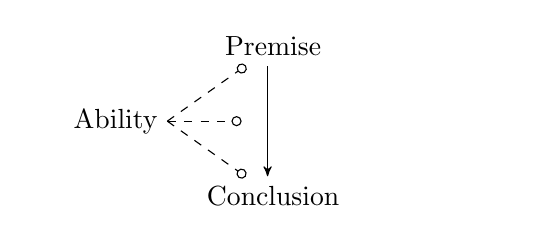
\begin{tikzpicture}[->, >=stealth', node distance=0cm, every text node part/.style={align=center}]
      \node [] (c) at (0,0) {};
      \node [] (d) at (-3,0) {};
      \node [] (e) at (3,0) {};
      \node [] (f) at (0,-2.1) {};

      \node (premise) at (0,-.1) {Premise};
      \node (conclusion) at (0,-2) {Conclusion};

      \node (x) at (-2,-1.05) {Ability};
      % \draw [->] (premise.270) to node[left] (3) {} (conclusion.90);
      \draw [->, xshift=-2] (0,-.35) to  node[right] {} (0,-1.75);

      % \node (4) [left of=3, xshift=-2cm] {};
      \draw [-{Circle[open]}, dashed] (x.0) to (premise);
      \draw [-{Circle[open]}, dashed] (x.0) to (conclusion);
      \draw [-{Circle[open]}, dashed] (x.0) to (-.4,-1.05);
    \end{tikzpicture}
    \caption{\WR{}}
    \label{fig:WR:support}
  \end{subfigure}
  \caption{Relations of support for \AR{} and \WR{}}
  \label{fig:ARandWR:support}
\end{figure}
\end{note}

\begin{note}[Difference with support]
  The significant difference is with support.
  \AR{} traces support from ability, while \WR{} traces support from premises available to the agent through to conclusion.
\end{note}

\begin{note}[Brief note on alternative]
  We do not claim that \AR{} and \WR{} are the only ways in which the agent may obtain support for conclusion.
  In particular,
  \begin{enumerate}
  \item Precondition of receiving information.
  \end{enumerate}
  In simple cases, all three may be available to an agent after receiving information.
  Case is designed with general to specific to rule out this option.
\end{note}

\subsection{\AR{}}
\label{sec:ar}

\begin{note}[The way to phrase this]
  Well, at some point the agent is in a position to attribute sufficient support to themselves.
  Start with the easiest case, ability, and then expand to other cases.
\end{note}

\begin{note}[Attribution]
  \AR{} establishes a relation of support between an agent's (specific) ability to reason to some conclusion, and some proposition which follows via potentive entailment.
  Take the information, and link.

  We have argued that potentive entailment is understood via preconditions for witnessing events of the ability.
  However, as the agent performs the action described by the verb, it makes sense to attribute the agent the property of being able, or in a position, to bring about the potential event.

  Properties are cheap.
  On my desk is a cup of coffee.
  The cup has the property of containing coffee.
  The coffee has the property of being in the cup.
  I have the property of having poured the coffee into the mug.
  Previous moments have the property of being moments for which I was pouring coffee in to the cup.
  And, I have the property of being in a position to drink the coffee in the cup.

  For sure, it's something that has not happened, but so long as there is sense to be made of a potential event, there's a corresponding property.

  Might reduce why this is true to something else, particular path of mental steps.
  But we're still going to have a property of this kind.

  Though potentive entailment is understood in terms of events, the property of being able to reason to some conclusion references some potential event and we may chain together a derived instance of potentive entailment.
  \begin{enumerate}
  \item As the agent has the (specific) ability, there is a potential event,
  \item Potential event only if \(\phi\) is a precondition of the potential event, therefore
  \item Agent has (specific) ability, \(\phi\) holds.
  \end{enumerate}
  As we are interested in the support appealed to by the agent, and not {\color{red} some kind of metaphysical} support relation, the derived instance of potentive entailment provides a route for the agent to transmit support they have for having the ability to the relevant precondition for the potential event.

  In short, it seems that derived potentive entailment is suitable for transmitting support.
  Whatever support the agent has for the (specific) ability also provides support for the preconditions for witnessing the (specific) ability.

  Countless examples.
\end{note}

\begin{note}[Ability is not strictly required for attribution]
  Described \AR{} with ability.
  Have seen that this can be reformulated in terms of potential event.
  The same pattern holds with potential event.

  For example, support for potential event, so conclusion holds.
\end{note}

\begin{note}[Example, fire]
  Alarm is ringing, so there is a fire.

  Same basic idea.
\end{note}

\begin{note}[Requires support for ability]
  Before turning away from \AR{}, let us stress that \AR{} requires the agent to have support for the (specific) ability in order to obtain support for the conclusion.
  Hence, if the agent does not have support for the (specific) ability, then they will not have the option of obtaining support for the conclusion via \AR{}.
\end{note}

\begin{note}[Relation to uRa]
  There is no immediate relation between \AR{} and~\ref{denied-claim}.

  \ref{denied-claim} talks about access to premises.
  \AR{} states that there is a support relation.

  \ref{denied-claim} enters the picture when observing that the agent has information about ability prior to witnessing ability.

  If the agent has information about (specific) ability and the agent has support for information, then extending support from ability to result is consistent with~\ref{denied-claim} as the only required premise is that the agent has the ability.
\end{note}

\begin{note}[Evidence of evidence]
  We have considered \AR{} from the perspective of potentive entailment.

  Variation.
  Following previous section, entailment.
  Support for support.
  Or, evidence of evidence.
\end{note}

\begin{note}[Evidence of evidence]
  \begin{quote}
    If E1 is evidence that E2 supports P, then E1 supports P.
  \end{quote}

  Trouble with this formulation.
  Following~\citeauthor{Feldman:2014un}
  Support that P entails Q, but it does not follow that this supports Q.
  Support for entailment, rather than consequent of entailment.
  (\citeyear[291]{Feldman:2014un})

  So, \AR{} is \emph{not} plausibly recast in terms of support for entailment providing support for conclusion.
  Rather, modify to include evidence for E2.

  \begin{quote}
    If E1 is evidence for E2 and E2 is evidence for P, then E1 supports P.\nolinebreak
    \footnote{
      \begin{quote}
        (EEE1) If E (non-conclusively) supports the claim that (some subject) S possesses evidence which supports p, then E supports p.\nolinebreak
        \mbox{}\hfill\mbox{(\citeyear[4]{Tal:2017uw})}
      \end{quote}
      Or, there is evidence.
    }
  \end{quote}

  So, information about ability provides evidence for premises, and then link comes for free, so to speak.

  Note that this is simply an instance of the previous version of \AR{} with an additional step.
  This is not true in general, but for our purposes we don't need to narrow the principle.\nolinebreak
  \footnote{
    Note to literature, esp.\ \citeauthor{Tal:2017uw}.
  }

  Remains a point of interest.
  Close to sketch of \WR{} made above, and described in more detail below.
\end{note}

\begin{note}[Evidence of evidence]
  Secondary interest is in \emph{de re} and \emph{de dicto}.
  Preparation for \WR{}.

  \citeauthor{Tal:2017uw} disambiguate \emph{de re} and \emph{de dicto} readings of EEE.
  Framed in terms of existence, in cases of interest, agent `has' the evidence/support.

  \begin{quote}
    For all \(e\) and \(p\), if \(e\) is evidence that there is evidence \(e'\) for \(p\), then \(e\) is evidence for \(p\).\nolinebreak
    \mbox{}\hfill\mbox{(\citeyear[8]{Tal:2017uw})}
  \end{quote}
  In example, this links the existence of premises.

  Support is not obtained from premises (which the agent has not reasoned from, and have not be `accessed'), but on the existence of premises for the conclusion (which the agent may `access' from potentive entailment).

  So, because existence we get support.

  \citeauthor{Tal:2017uw} suggest \emph{de dicto}.
  \begin{quote}
    For all \(e\), \(e'\) and \(p\), if
    \begin{enumerate*}[label=(\roman*), ref=(\roman*)]
    \item \(e\) is evidence for \(e'\) and
    \item \(e'\) is evidence for \(p\),
    \end{enumerate*}
    then \(e\) is evidence for \(p\).\nolinebreak
    \mbox{}\hfill\mbox{(\citeyear[8]{Tal:2017uw})}
  \end{quote}
  In example, this links the premises themselves.
  Premises do provide support.
  Here, this is close.
  The core idea of \WR{} is that the premises do the work.

  So, then, this provides an account that is somewhat close.
  Important thing is that the support transfers through to ability.

  Initial sketch will follow in this lines.
  Difficulty is with doxastic support.

  Granting propositional support \dots
  Seems agent is going to require support for ability in order to get conclusion.
  So, propositional aspect corresponds with \WR{}, but doxastic does not.
\end{note}

\begin{note}[Broader narrative]
  We've offered a variety of ways to understand \AR{}.
  Common thread is that the agent obtains support for conclusion from support for ability.

  EEE.
  Provided an variant of \AR{} when understood \emph{de dicto}.
  Similar to \WR{} when understood \emph{de re}, but remained issue with doxastic support.
\end{note}

\subsection{\WR{}}
\label{sec:wr}

\begin{note}[Overview]
  In section~\ref{sec:ar-wr} we outlined the key distinction between \AR{} and \WR{} for the purpose of the overarching argument of this thesis.

  Understanding \WR{}.
\end{note}

\begin{note}[General idea of \WR{}]
  The core idea of \WR{} is that the agent uses information that there is a potential event in order to claim support for the conclusion.

  The potential event involves the agent reasoning to some conclusion.
  Reasons from premises.

  As event of reasoning is potential, preconditions are satisfied.
  Hence, conclusion holds, and premises sufficient for conclusion in line with \USE{}.


  The agent does not rely on support for there being a potential event, or support for having an ability, as in the case of \AR{}.
\end{note}

\begin{note}[Negative characterisation of \WR{}]
  Negative characterisation of \WR{} in terms of support that the agent does not appeal to.
  So, no support which goes straight to the conclusion.
\end{note}



\begin{note}[Two passes]
  Two passes at \WR{}.
  First pass assumes understanding of propositional support.
  In cases discussed, agent has option of appeal to independent propositional support for premises of reasoning.
  Core idea of \WR{} is that potential event of reasoning allows agent to extend to propositional support for the conclusion of reasoning.

  The core idea of \WR{} has a two primary purposes.
  As noted, allowing support.
  Also, going for things in the right way\dots

  Primary purpose of first pass is to introduce ideas.
  Understand the role of information as allowing a particular closure relation with respect to propositional support.

  Observe that this requires a particular understanding of propositional support, and criticise the pass for insufficient motivation even if understanding of propositional support is adopted.

  Leads to a second pass in which we introduce idea of deferred support.
  Core idea of deferred support is that link is created, but establishing the link is deferred.
  Role of information is in allowing the agent to defer establishing relation.

  Support `just is' the deferred support from establishing.
  `Little more' than temporal separation.

  Second pass is fairly minimal.
  E.g.\ doesn't depend on understanding of propositional support.
  One may (of course) add further conditions.
  Hence, pursue as sufficient, but real interest is in idea of deferring, whether or not this needs supplementation.
\end{note}

\begin{note}[No inherent conflict]
  These passes do not inherently conflict with~\ref{denied-claim}.

  Simplest to see in cases of memory loss.
  Provide some motivating independent of the intended application.
  Although true for both passes, delay discussion for second pass.

  Key is that these passes make room for conflict.

  Passes do conflict with a stronger refinements of~\ref{denied-claim}.
\end{note}

\subsubsection{First pass: Propositional support}
\label{sec:first-pass:-prop}

\begin{note}[Recap]
  Type of situations.
  Some general ability.
  Conditional information.
  Conclusion.
\end{note}

\begin{note}[Core idea]
  The motivating idea for our first pass at a detailed understanding of \WR{} is that so long as the information is true, then the agent has propositional support for conclusion.
  Following proposition/doxastic distinction is appropriate connexion.
  Appropriate connexion does not added support, rather allows the agent to make use of support.
  Appeal to potential event/ability allows agent to anticipate appropriate connexion.
  Hence, something a little weaker than doxastic support.

  Three important points here.
  \begin{enumerate}
  \item propositional support.
  \item information that propositional support.
  \item additional features connect agent to propositional support, and do not add support.
  \end{enumerate}

  Idea is that agent appeals to propositional support that they have.

  Key point of argument is that if agent has propositional support, then that is sufficient support for conclusion.
  Agent appeals to propositional support, which is premises.
  Role of \WR{} is in granting connexion between premises and conclusion.
\end{note}

\begin{note}[Propositional and doxastic support]
    Our use of support falls closer in line with doxastic justification as opposed to propositional justification.
  Roughly, following \textcite{Silva:2020aa}:

  \begin{quote}
    \textbf{Propositional Justification}: S has propositional justification to believe that p iff
    \begin{itemize}
    \item S has sufficient epistemic reasons to believe that p.
    \end{itemize}

    \textbf{Doxastic Justification}: S has a doxastically justified belief in p iff
    \begin{enumerate}[label=(\roman*), ref=(\roman*)]
    \item\label{dj:def:i} S has propositional justification to believe that p,
    \item\label{dj:def:ii} S believes that p, and
    \item\label{dj:def:iii} S's belief in p is appropriately connected to S's sufficient epistemic reasons to believe p.
    \end{enumerate}
  \end{quote}

  These are fairly neutral definitions.
  Basic idea is that the agent has propositional support, and doxastic support traces this.

  \USE{} informs our understanding of sufficient epistemic reasons.
  So long as agent has reasoned, then those premises (and perhaps steps used, maybe lack of other premises) are sufficient epistemic reasons.
  No need for full account.
  In turn, ability/potential event involves sufficient epistemic reasons.

  Important point here is that propositional support alone doesn't do much.
  An agent may have propositional support for some proposition and either not recognise that they have propositional support, or fail to form any attitude toward the proposition in line with the propositional support they have.
\end{note}

\begin{note}[P/D Example]
  To illustrate the distinction between propositional and doxastic support, consider the following multiple choice question.

  \begin{figure}[H]
    \centering
    {
      \sffamily
      \newcommand{\pythagwidth}{3cm}
      \newcommand{\pythagheight}{5cm}
      \begin{tikzpicture}[box/.style={rectangle, rounded corners, draw=black, text width=15mm}]
        \begin{scope}[shift={(0,0)},rotate=270, scale=0.75]
          \coordinate [label={below right:}] (A) at (0, 0);
          \coordinate [label={above right:}] (B) at (0, \pythagheight);
          \coordinate [label={below left:}] (C) at (-\pythagwidth, 0);

          \coordinate [label={below:\(5\text{cm}\)}] (F) at (0,\pythagheight/2);
          \coordinate [label={left:\(3\text{cm}\)}] (G) at (-\pythagwidth/2, 0);

          \coordinate (D1) at (-\pythagheight, \pythagheight + \pythagwidth);
          \coordinate (D2) at (-\pythagheight - \pythagwidth, \pythagwidth);

          \draw [] (A) -- (C) -- (B) -- (A);
          \newcommand{\ranglesize}{0.3cm}
          \draw [line width=0.4pt] (A) -- ++ (0, \ranglesize) -- ++ (-\ranglesize, 0) -- ++ (0, -\ranglesize);
        \end{scope}

        \node (Answer) at (7,1.25) [text width=6cm]
        {
          What is the area of the given triangle?
          \begin{enumerate}[label=\Alph*.]
          \item \(4\text{cm}^{2}\)
          \item \(7.5\text{cm}^{2}\)
          \item \(16\text{cm}^{2}\)
          \end{enumerate}
        };
        \draw [rounded corners] (-1,-.5) -- (10,-.5) -- (10,2.75) -- (-1,2.75) -- cycle;
      \end{tikzpicture}
      \vspace{5pt}
    }
  \end{figure}

  \noindent The students have been taught:
  \[\text{Area of triangle} = \left[\sfrac{1}{2} \times \text{base} \times \text{perpendicular height}\right] (\text{square units})\]
  Perhaps the students have testimony of teacher, or perhaps have been given a proof.
  Either way, applied to given triangle provides sufficient epistemic reasons, and for simplicity \emph{stipulate} no other epistemic reason.\nolinebreak
  \footnote{Somewhat tricky as there may be ways to eliminate the two other options.
    Stipulate in order to ease a point made below.
  }

  Three variations.
  No propositional (entails no doxastic).
  Propositional and doxastic.
  Propositional and no doxastic.

  Consider a handful of students.
  First, guesses.

  remaining four clarify divide.
  First pair, clear instances.
  Second pair, more difficult cases.
  First is great case.
  Guess again, clearly no dox, though prop.

  Two students who have applied the formula, and calculated that \(\sfrac{1}{2} \times 5\text{(cm)} \times 3\text{(cm)} = 7.5(\text{cm}^{2})\).
  Both students have the correct answer.
  However, only one of the students has noted that \(3\text{cm}\) may be taken as the (perpendicular) height of the triangle because the triangle is a right angle.
  The other student has taken \(3\text{cm}\) to be the (perpendicular) height of the triangle because it is the length of one edge of the triangle.
  The student understands that the perpendicular height of a triangle may differ from the length of any given edge of a triangle, but due to exam pressure has overlooked this possibility.

  As both students understand how to apply the formula they have been taught, it seems both students have propositional support for the answer they have given.
  However, it seems only the former student also has doxastic support for the answer they have given.
  The latter student has the correct answer.
  However, the latter student's belief that the area of the triangle is \(7.5\text{cm}^{2}\) is not appropriately connected to the student's epistemic reasons to believe that the area of the triangle is \(7.5\text{cm}^{2}\).
  For, if the question had been altered so that the triangle was not a right angled triangle, the latter student would not have arrived at a misleading belief about the area of the triangle given the reasoning performed.\nolinebreak
  \footnote{
    Note, not saying that the student would not have arrived at the correct answer.
    For, the student may have clarified their reasoning if the answer given did not match a choice.
    Rather, if the same reasoning was applied (with different lengths) to a non-right angled triangle, the agent would not have correctly identified the perpendicular height of the triangle.
  }

  Third student who did not understand the formula but has it written down on a cheat sheet.
  The student sees that calculating the area of a triangle involves multiplying two numbers and dividing the result by two, and so believes that the area of the triangle is \(7.5\text{cm}^{2}\) because the only two numbers available are odd, recalls the result of multiplying two numbers is always odd, and that division by two of any odd (rational) number must involve a fraction.
  Certainly no doxastic support.

  Fourth student, guesses.

  Without a full account of sufficient epistemic reasons, unclear that the student has propositional justification.
  As the student did not understand the formula, lack sufficient epistemic reasons.
  However, possible to allow as the formula is in front of the student.\nolinebreak
  \footnote{Compare \citeauthor{Firth:1978vi}'s example with Holmes and Watson (\citeyear[218]{Firth:1978vi}).
    Watson is presented with all the evidence Holmes used to that the coachman committed the murder, and that this provides Watson with sufficient epistemic reasons regardless of whether or not Watson forms any attitude, but it is not clear that Watson has the understanding to piece together the evidence laid before them.}

  A clearer case of a student who lacks even propositional support may be a student who forms a belief that the area of the triangle is \(7.5\text{cm}^{2}\) without learning the formula, but because it is one of the options given, and one in four odds aren't too bad.
  No possibility of doxastic support.

  No stance on borderline cases.
  Rather, helpful because this highlights how two important conditions work.
  What it is to have sufficient epistemic reasons, and what it is for an agent's belief to be appropriately connected to the agent's sufficient epistemic reasons to believe.
\end{note}

\begin{note}[Takeaway]
  Student who have propositional support have so independently of whether the way they form a belief is appropriately connected.
  Whether doxastic considers how the agent forms the belief.

  Relation to cases of interest.
  If the information is true, then the agent has propositional support.
  For, result of reasoning would be good, and potential means that there's no opportunity to acquire new information.

  Agent does not have doxastic support.
  Some flexibility on what the third condition amounts to, but the overall argument is that there is an exception to~\ref{denied-claim}.
  Noted problems with basing.
  I see no interest in arguing that the term `doxastic support' applies to cases of interest.
  Given well-developed analyses of the basing relation, then leaves `doxastic support' to those analysis.

  Doxastic support requires an \emph{appropriate} connexion, but `appropriate' is one adjective among many.
  There are other adjectives --- or ways in which the agent may relate sufficient epistemic reasons to conclusion --- that may be of interest.

  Further, if information is true, then potential event seems a clear case.
  Unlike the second pair, things aren't too delicate.
  Agent reasons well, and potential event so avoid worries about the degree to which propositional support is in reach.
\end{note}

\begin{note}[Generalising a little]
  Propositional support is focus.
  Given definition, applies to p, some proposition.
  Extend to cover steps of reasoning.
  May always reduce to a proposition, if given some basic.
  Still, talk of steps.
\end{note}

\begin{note}[Agent doesn't need support to appeal to support]
  This is super important to stress that agent doesn't need support to appeal to support.
  Mistakes are made, even when reasoning.
  One uses a premise which one doesn't have propositional support for.
  For example, by something changing in the world.
\end{note}

\begin{note}[Where this is going]
  With a (sufficiently) neutral distinction between propositional and doxastic support in hand, we now turn to an argument for the claim that the agent is in a position to form an attitude to conclusion, where support appealed to are those premises that would be used in reasoning.

  For the agent to obtain doxastic support, need appropriate connexion, not additional support.

  Independent relation of propositional support between premises and conclusion.
  Premises --- whatever these happens to be --- provide the agent with propositional support for the conclusion, independent of whether the agent has, or will, do the reasoning.
  Conditional information, provides agent with information that general ability provides access to propositional support.
  That is, whatever the propositional support happens to be, if the information is true then the agent has access to propositional support.
  On a standard picture, the agent obtains doxastic support from propositional support if attitude toward conclusion is appropriately connected to propositional support.
  What is missing is an appropriate connexion.

  That is, two components.
  \begin{enumerate}
  \item Support
  \item How the agent uses this support to get conclusion.
  \end{enumerate}

  If information is true, then as the agent already has sufficient support for the conclusion on basis of premises, our task is to explain how information about ability/potential event allows the agent to appropriately connect attitude toward conclusion to premises.

  Propositional support alone doesn't do much.
  But the information is useful.
\end{note}

\begin{note}[Idea]
  Idea is to show that the agent may appeal to having propositional support for whatever the premises of reasoning are.
  Information then used to extend propositional support for premises to propositional support for conclusion.
  In turn, attitude toward conclusion based on propositional support, whatever that propositional support happens to be.

  Four key points to the argument, which we will work through.
  \begin{enumerate}[label=(V\arabic*), ref=(V\arabic*)]
  \item\label{W:fp:S:1} If there is a relation of propositional support between premises and conclusion of reasoning, then witnessing the reasoning does not provide an agent with \emph{additional required} support for the conclusion.\nolinebreak
    \footnote{May provide the agent with additional support, but it isn't required for the agent.}
  \item\label{W:fp:S:2} If support for general ability, agent may (plausibly) appeal to having propositional support for any premises or steps of reasoning which is an exercise of the relevant general ability.
  \item\label{W:fp:S:3} A potential event of witnessing is sufficient for the agent to hold that propositional support for premises of reasoning extend to conclusion.
  \item\label{W:fp:S:4} Attitude that conclusion is true based on propositional support for conclusion (and not that the agent has attitude toward propositional support).
  \end{enumerate}
  The four key points are then unified by the following pair of observations:
  \begin{itemize}
  \item From~\ref{W:fp:S:1} and~\ref{W:fp:S:2}, agent may hold that they have propositional support for conclusion.
  \item From~\ref{W:fp:S:3} and~\ref{W:fp:S:4}, Attitude toward conclusion based on premises used when witnessing.
  \end{itemize}
  Second observation may also use~\ref{W:fp:S:2}, given steps that would be used in reasoning.

  Figure~\ref{W:fp:steps:diagram} provides a (rough) visual representation of how the four steps fit together.
\end{note}

\begin{figure}[H]
  \centering
  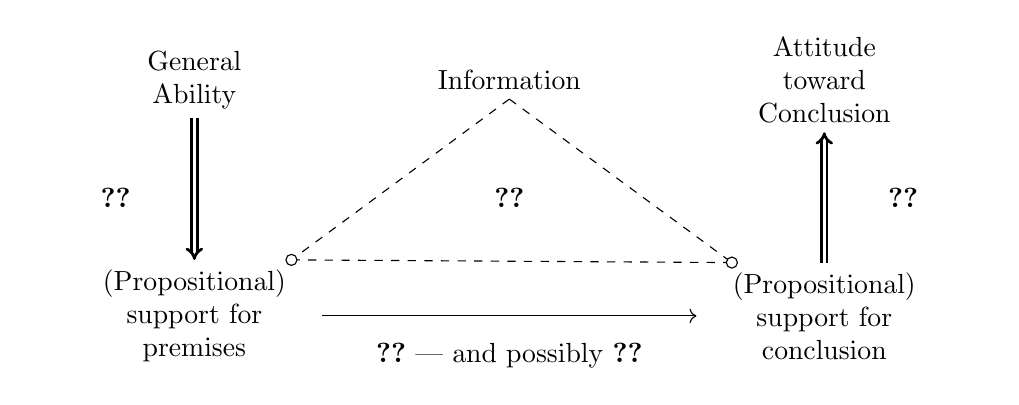
\begin{tikzpicture}[scale=.5]
    \node at (0,0) (GA) {\parbox{2cm}{\centering General Ability}};
    \node at (8,0) (I) {\parbox{2cm}{\centering Information}};
    \node at (16,0) (AC) {\parbox{2cm}{\centering Attitude toward Conclusion}};


    \node at (0,-6) (PP) {\parbox{3cm}{\centering (Propositional) support for premises}};
    % \node at (8,6) {\parbox{3cm}{\centering Information}};
    \node at (16,-6) (PC) {\parbox{3cm}{\centering (Propositional) support for conclusion}};

    \node at (-2,-3) {\parbox{2cm}{\centering \ref{W:fp:S:2}}};
    \node at (8,-7) {\parbox{6cm}{\centering \ref{W:fp:S:1} --- and possibly~\ref{W:fp:S:2}}};
    \node at (18,-3) {\parbox{2cm}{\centering \ref{W:fp:S:4}}};
    \node at (8,-3) {\parbox{2cm}{\centering \ref{W:fp:S:3}}};

    \draw [-Implies,line width=1pt,double distance=1pt] (GA) -- (PP);
    \draw [-Implies,line width=1pt,double distance=1pt] (PC) -- (AC);
    \draw [->] (PP) -- (PC);

    \draw [-, dashed] (PP.30) -- (PC.150);
    \draw [-, dashed] (I.270) -- (PP.30);
    \draw [-, dashed] (I.270) -- (PC.150);

    \node[circle,draw=black, fill=white, inner sep=0pt,minimum size=4pt] (b) at (PP.30) {};
    \node[circle,draw=black, fill=white, inner sep=0pt,minimum size=4pt] (b) at (PC.150) {};
  \end{tikzpicture}
  \caption{Representation of important steps}
  \label{W:fp:steps:diagram}
\end{figure}

\begin{note}[Explaining figure]
  Trace the arrows.

  Top line, what the agent accesses.
  Bottom line, support.
\end{note}

\begin{note}[First key point]
  The first key point states:
  \begin{enumerate}
  \item If there is a relation of propositional support between premises and conclusion of reasoning, then witnessing the reasoning does not provide an agent with \emph{additional required} support for the conclusion.
  \end{enumerate}
  The point follows from the definitions of propositional and doxastic support, and independently of any particular account of what sufficient epistemic reasons are (or what support is).

  For, conditions~\ref{dj:def:i} and~\ref{dj:def:iii} of the given definition of doxastic support states that the agent has propositional support to believe that p, or equivalently that the agent has sufficient epistemic reasons to believe that p, given the definition of propositional support.
  Therefore, if sufficient epistemic reasons relied on additional (epistemic) reasons introduced by either condition~\ref{dj:def:ii} or condition~\ref{dj:def:iii}, then either:
  \begin{enumerate*}[label=(\roman*)]
  \item The sufficient epistemic reasons identified by the agent having propositional support are not sufficient for holding an attitude toward the conclusion --- a contradiction.
    Or
  \item The definitions of propositional and doxastic support are equivalent.
  \end{enumerate*}

  Assume for equivalence that some collection of the conditions for doxastic support introduce additional required support for the conclusion.
  As the epistemic reasons identified by propositional support are sufficient, then given the assumption made, propositional support must reference doxastic support in order to identify the additional epistemic reasons introduced by some collection of the conditions for doxastic support in order for the agent to have sufficient epistemic reasons to hold an attitude toward the conclusion.
  However, doxastic support in turn requires the agent to have propositional support by condition~\ref{dj:def:i}.
  So, in order for the agent to have doxastic support the agent must have propositional support, but given the assumption, in order for the agent to have propositional support, the agent must have (some part of) doxastic support.

  There need not be anything problematic with circular definition.
  Rather, the observation is that if the definitions are circular in this way, then the presence of condition~\ref{dj:def:i} as part of the definition of propositional support allows one to eliminate either either condition~\ref{dj:def:ii}, condition~\ref{dj:def:iii}, or both from the definition of doxastic support.

  Note, however, that condition~\ref{dj:def:iii} requires condition~\ref{dj:def:ii} to be true, as the agent's belief is required to be appropriately connected to the agent's sufficient epistemic reasons.
  Therefore, it seems that if condition~\ref{dj:def:iii} is a required epistemic reason then condition~\ref{dj:def:ii} must also be a required epistemic reason.
  Hence, the definitions collapse in to one another and there is no distinction between propositional and doxastic support.

  So, then leave out condition~\ref{dj:def:iii}, but this is the condition where things are different.
  Only appropriate connexion without further information would be reasoning, by~\ref{denied-claim}.
  Hence, given definitions and difference, then result wanted.

  As doxastic is the attitude, proposition is supported independently of whether or not the agent has reasoned.\nolinebreak
  \footnote{
    This is not to say that the agent is irrelevant. (Notably observed by \cite{Firth:1978vi} when introducing the terminology).
    Rather, that the agent has (propositional) support whether or not they have reasoned.
  }
  Therefore, as we're dealing with a potential event, then given the definitions of propositional and doxastic support \emph{and} given the truth of the information, then the agent has propositional support for the conclusion, no matter what sufficient epistemic reasons turn out to be.
\end{note}

\begin{note}[Closure principle]
  Summarise with a closure principle for propositional support:
  \[\propsupp{\phi} \land (\phi \ientails{} \psi) \vdash \propsupp{\psi}\]
  If reasoning would lead to conclusion, and agent has support for premises, then agent has support for conclusion.
  
  This simply states things about propositional support.
  Closure principles, because it states that \(\psi\) is a member of the class of things that are propositionally justified.
\end{note}

\begin{note}[Slight problem]
  This premise is important, but fairly weak.
  May be the case that the agent is required to reason to have propositional support (i.e.\ sufficient epistemic reasons).
\end{note}

\begin{note}[Concludes first step]
  This is the first step.
  Given definitions of propositional and doxastic support, the agent is not required to reason in order to have sufficient epistemic reasons for the conclusion.
\end{note}

\begin{note}[Second step]
  Second step:
  \begin{enumerate}
  \item[\ref{W:fp:S:2}] If support for general ability, agent may (plausibly) appeal to having propositional support for any premises or steps of reasoning which is an exercise of the relevant general ability.
  \end{enumerate}
  Phrased a little more naturally, though perhaps a little more controversially:
  \begin{enumerate}
  \item[\ref{W:fp:S:2}] In the scenarios of interest, the agent may (plausibly) \emph{believe} they have propositional support for any premises or steps of reasoning which is an exercise of the relevant general ability.
  \end{enumerate}
  Prefer to stay neutral.
  Still, highlighting belief, repeat a clarification from earlier.
  \ref{W:fp:S:2} does not require the agent to have support.
  Rather, \emph{appeal} to having propositional support.
  No plausible requirement that an agent may appeal to propositional support only if they do have propositional support.
  Motivated with changes to environment.

  Same applies to cases.
  Agent has support for general ability.
  May not have propositional support.

  Two examples.

  Agent has been taught, and teacher is bad.
  Agent does not have propositional support, but fair for the agent to appeal to having propositional support.

  Agent has learnt majority of rules, feedback that these are complete.
  However, additional rule stating an exception to rule that has been learnt.
  Given that the rules of chess are fairly compact, this takes some imagination, but provided some examples earlier.
  Seems plausible that the agent may appeal to having propositional support as from agent's perspective there.

  Still, as noted in concluding first key point, something substantial needs to be said about sufficient epistemic reasons in order for this second key point.
  Hence, role of qualifier.
  No direct argument.

  Here, rely on~\USE{} again, though slightly expanded.
  Premises, or steps of reasoning are sufficient epistemic reasons.
  Nothing more to support with respect to reasoning.

  Consider validity.
  If Premises are true, then conclusion is true.

  Steps are fixed.
  Allow different steps.
  If Premises are true, and steps preserve truth, then conclusion is true.

  Soundness.
  Premises are true, steps preserve truth, then conclusion is true.

  Truth, but more generally some designated property.
  E.g.\ probability, or desirability.

  Vary from preservation.
  What matters is that the conclusion has the designated property.
  (May be probability example for this.)

  So, premises and steps are sufficient to ensure that conclusion has designated property.

  Concerns about what is required for ensuring, but hard to think of there being something in addition to premises and steps which is relevant to ensuring designated property.

  So, reasoning/demonstration (and hence exercise of general ability) is understood in terms of premises and steps.

  Granting this, question is whether agent may appeal to having propositional support from exercise of general ability.

  Role of general ability has two parts.
  First, no new information --- this is a strict reading.
  Already seen that propositional support/sufficient epistemic reasons whether or not agent reasons.
  Second, the agent doesn't stray from premises and steps that they (may claim to) have support for.

  This seems to capture something unremarkable.
  Consider arithmetic.
  \(((421 + 531) \times 5)/7\).
  General ability, so if you calculate, you will get the right answer.\nolinebreak
  \footnote{
    \(((421 + 531) \times 5)/7\) = \((300 + 40) \times 2\)
  }
  Checking propositional validity.

  Short term memory, names of people in a group.
  So long as group isn't too big, and names are familiar.

  Most common, parsing novel sentences.
  Take some book designed to teach reading.
  Some novel sentences, but understanding meaning.
  Somewhere on the way to The Waste Land this breaks down.
  Compositionality.

  Consider converse cases.
  Cases of reasoning where there is a necessary step or premise, and the agent lacks support.
  E.g.\ misunderstood a particular rule.
  Agent lacks support, and recognised, then lack general ability.

  Likewise, non-reasoning cases.
  Cooking.
  Experience, various recipes and styles, good dishes.
  Some general ability, mastered some skills.
  As long as novel recipe only requires those skills, expect the meal to turn out well.

  Perhaps agent may not have the skill to articulate support appealed to, but still appeal.
\end{note}

\begin{note}[Second pair of key points]
  We now turn to the remaining two key points.
  This is where things get a little more complex.
\end{note}


\begin{note}[Third key point]
  Previous key point~\ref{W:fp:S:2}, agent has propositional support for any premises and steps used when witnessing general ability.
  \ref{W:fp:S:1}, witnessing doesn't add.
  Third key point builds on~\ref{W:fp:S:1} and \ref{W:fp:S:2} given information about potential event of witnessing general ability.
  \begin{enumerate}
  \item[\ref{W:fp:S:3}] Information of a potential event of witnessing is sufficient for the agent to hold that propositional support for premises of reasoning extend to conclusion.
  \end{enumerate}

  In broad strokes, from~\ref{W:fp:S:1}, propositional support/sufficient epistemic reasons do not require reasoning.
  Therefore, if reasoning would lead to conclusion, and agent has support for premises, then agent has support for conclusion.
  Saw this with closure.

  From~\ref{W:fp:S:1}, if information is true, then attitude to antecedent condition of closure.
  Main claim is that agent does not require support for reasoning to extend attitude toward conclusion and form attitude toward consequent of closure condition.

  Here, the idea of \WR{}.
  Not strictly a propositional attitude.
  Instead, appeal to the potential event of witnessing reasoning.
  Ties attitude toward conclusion to that reasoning.
  That is, whatever those reasons are which are sufficient for propositional support, if agent does have propositional support.

  Second point is important.
  For, agent is appealing to \WR{}, hence relying on support for general ability as applied, rather than obtaining support for specific ability.

  {
    \color{red}
    {\color{green} This note needs to be cleaned up and stated in various other places.}
    Delicate.
    The agent is not obtaining support for specific ability.
    Instead, the agent is appealing to support for general ability that would be used if they were to witness the specific ability.
    Further, result is not immediately that the conclusion is true, but that the agent has propositional support for conclusion.

    Problem with support for specific ability was reasoning that otherwise the agent support would be misleading.
    Insight is that agent doesn't need to go directly to specific ability, as it may be built from elements of general ability.
    \WR{} is the key piece where the agent considers reasoning, and how the general ability interacts.
    Without witnessing, no appeal to the steps of reasoning, and support agent has for these.
  }
\end{note}

\begin{note}[Relation to closure]
  Begin by returning to closure principle for propositional support:
  \[\propsupp{\phi} \land (\phi \ientails{} \psi) \vdash \propsupp{\psi}\]
  This simply states things about propositional support.
  Closure principles, because it states that \(\psi\) is a member of the class of things that are propositionally justified.
  There's nothing about an agent's recognition in play here.

  To ease introduction of attitudes, consider an easier case.
  Knowledge.
  \[K(\phi) \land K(\phi \rightarrow \psi) \vdash K(\psi)\]
  Natural language, if agent knows that \(\phi\) and knows that \(\phi\) entails \(\psi\), then the agent knows that \(\psi\).
  Knowledge is factive.
  Note, switch to entailment, as proposition.
  So, it must (given agent's knowledge) be the case that \(\phi\) and that \(\phi\) entails \(\psi\), and hence it must be the case that \(\psi\).\nolinebreak
  \footnote{
    Variations on epistemic closure principle which do not require \(\geop{2}\).
    E.g.\ \citeauthor{Williamson:2000wx} formulates \emph{intuitive closure} as:
    \begin{quote}
      knowing \(p_{1},\dots,p_{n}\), competently deducing \(q\), and thereby coming to believe \(q\) is in general a way of coming to know \(q\).\nolinebreak
      \mbox{}\hfill\mbox{(\citeyear[117]{Williamson:2000wx})}
    \end{quote}
    Multi-premise, perhaps fine with knowledge, we restrict to single premise for the moment.

    \citeauthor{Hawthorne:2005tb}, generalisation
    \begin{quote}
      If one knows P and competently deduces Q from P, thereby coming to believe Q, while retaining one's knowledge that P, one comes to know that Q.\nolinebreak
      \mbox{}\hfill\mbox{(\citeyear[29]{Hawthorne:2005tb})}
    \end{quote}
    In terms of the formalism used:
    \[K(\phi) \land (\phi \ientails{} \psi) \Vdash K(\psi)\]

    \citeauthor{Hawthorne:2005tb}'s generalisation is important.
    Take similar restrictions to be implicit in main body.
    
  }

  Note, we're not interested in an unrestricted closure principle.
  Rather, observing that so long as some closure principle is true, then this seems to be an instance.

  Introduce a variant with propositional support.

  \[K(\propsupp{\phi}) \land K(\phi \rightarrow \psi) \vdash K(\propsupp{\psi})\]
  Natural language, if an agent knows that they have propositional support for \(\phi\), and the agent knows that \(\phi\) entails \(\psi\), then the agent knows that they have propositional support for \(\psi\).\nolinebreak
  \footnote{
    Originally in terms of belief, but as noted {\color{red} need to add}, generalises to other attitudes.
  }
  Here, reasoning as before, with the observation from~\ref{W:fp:S:1} that whatever secures knowledge of \(\phi\) provides sufficient epistemic reasons for \(\psi\), given possibility of reasoning.

  Use \(\Vdash\) to indicate permissibility of forming attitude to the right given attitudes to the left.

  \[K(\propsupp{\phi}) \land K(\phi \rightarrow \psi) \Vdash K(\propsupp{\psi})\]

  Example of difference.
  First, something standard.
  Second, knowledge of propositional support.
  Mnemonic for order of colours of the rainbow.
  Propositional support, sufficient epistemic reasons for order of colours of the rainbow.
  {
    \color{red}
    Might be easier with conditional structure and consequent.
  }

  May seem that the agent simply knows.
  Additional point in anticipation of next key point is that \(K(\propsupp{\phi}) \vdash K(\phi)\).
  Seems there's an equivalence here, as the converse certainly holds.
  Suggests that there aren't cases from perspective of attitude,  idea behind example, still, is different epistemic reasons.

  Perhaps clearer with potential event.
  If agent knows they have specific ability, then knows they have propositional support.
  However, as seen agent may then appeal to potentive entailment.
\end{note}

\begin{note}[Generalise closure]
  Return to \(\ientails{}\) and introduce some placeholders.

  \[\geop{1}(\propsupp{\phi}) \land \geop{2}(\phi \ientails{} \psi) \Vdash \geop{3}(\propsupp{\psi})\]

  Natural language, \dots
  Again, \(\Vdash\) to indicate permissibility of forming attitude to the right given attitudes to the left.

  Question is whether there are instances of \(\geop{1}\), \(\geop{2}\), and \(\geop{3}\), in parallel to \(K\).

  As with knowledge, not looking for general closure principle.
  Rather, there are cases.
\end{note}

\begin{note}[Claiming for \(\geop{1}\)]
  Talked in terms of claiming support.
  This provides instances for \(\geop{1}\).

  \[C(\propsupp{\phi}) \land \geop{2}(\phi \ientails{} \psi) \vdash \geop{3}(\propsupp{\psi})\]
  If agent claims propositional support for premises, some relation to reasoning, then some attitude toward conclusion.
\end{note}

\begin{note}[\(\geop{2}\)]
  \(\geop{2}\) is where \WR{} is important.

  From~\ref{W:fp:S:2}, plausible that the agent has support for any premises and steps following instance of general ability.

  Intuitive idea behind instance of \(\geop{2}\) is that it allows agent to appeal to premises and steps used in reasoning.

  Introduce \(W\).

  \[C(\propsupp{\phi}) \land W(\phi \ientails{} \psi) \vdash \geop{3}(\propsupp{\psi})\]

  Understanding of \(W\) is witnessing.
  Agent is committed to potential event, and hence committed to witnessing the reasoning.
  (Recall \nI{} limits this to commitment.)
  \(W\) claim support for each premise or step of event.

  Important here is that the agent is not directly claiming support for ability, so to speak.
  Rather, endorses potential event, which reduces down to parts.
  Agent is only claiming support for parts.

  Observation is that by viewing from this perspective, agent is in a position to claim (proposition) support for parts, given understanding of propositional support.

  Consider~\nI{} again.
  Trouble because the agent does not have the option of obtaining support for specific ability from general ability.
  The agent may not be able to do the reasoning.
  This may show that the agent does not have the general ability.
  May be misleading.
  Subtle, but important, difference is\dots that\dots agent is appealing to direct support.
  Problem with simple reasoning is that it's indirect --- the agent doesn't do anything with how the general ability extends.

  Given \(W\), then if the agent is misleading, then the trouble is same as if the agent performed the reasoning.
  There is a mistake with some premise or step.
  Important is that the agent is not appealing to not being misleading.
  Rather, the agent is appealing to use of general ability.
  Again, given \(W\) appealing to the propositional support, or sufficient epistemic reasons that the agent is in a position to claim that they have.

  Of course, if agent does not have general ability, then no witnessing.
  So, failure cases is not the same as agent reasoning with a misleading, but supported, premise or step.
  Agent may not reach conclusion.
  This may be why the agent gives up general ability when attempting to witness.
  Still, \emph{prior} to witnessing, this isn't so much of an issue.
  Given support for general ability, it is true that there's a potential event.

  Indeed, this distinguishes.
  \(W\) may fail in this way.
  As agent has not done reasoning, then may be that it is not possible for agent to reason.
  E.g.\ case of devious informer.

  However, this doesn't need to say much about how support works given \(W\).
  Return to \(K\).
  May turn out that one doesn't \(K\) that \(\phi\).
  So long as one does, the possibility of revising \(K\) doesn't show that the agent is not in a position to trace support from \(\phi\).

  {\color{red} As motivated} the role of witnessing is to apply general ability directly, so to speak.

  {
    \color{green}
    Does the agent get support for specific ability in this way?
    Arguably not, maybe, because \(W\) still has an important role.
    Then, there remains a significant puzzle about why the agent is in a position to claim support for conclusion.

    Okay, so agent falls short of support for ability because of \(W\).
    However, still gets support for conclusion?
    Well, so long as the agent is required to endorse, then so far the idea has been that the agent doesn't need to do the reasoning.

    So, \(W\) is doing \emph{something} important.
    It's something about non-voluntarism.

    Broken down and seen how the agent can't really avoid.
    Application of general ability really is supporting.
  }




  Agent is not appealing to support for general ability.
  Rather, how general ability functions when applied.
  Not support for general ability, per se, but rather support for premises and steps.

  Conflict with~\ref{denied-claim} is that the agent is not aware of what those premises and steps are.




  Why this doesn't require support.

  The important aspect of~\ref{W:fp:S:3} is that information is sufficient.
  So, information that this follows from general ability.

  For, then agent either gives up general ability, or is required to hold that they have ability.
  Of course, no support.

  So, as long as general ability, is potential event.
  However, and quite important, is that the agent is not obtaining support for specific ability/potential event on the basis that their support for general ability would be misleading.
  Rather, agent is observing that so long as it is true that there is a potential event, then support for general ability means that the agent has support they may appeal to when witnessing reasoning.

  Delicate, but the agent is not generating support for a novel proposition that they have specific ability, as would be the case with ability.
  Instead, observation is that the support they already have applies to novel proposition that conclusion is true.

  From this perspective, information is merely directing the agent as to \emph{what} follows from general ability.

  Summary of \(W\), then, is that permissible for agent to have attitude of \(W\) toward reasoning just in case support for stages.
\end{note}

\begin{note}[\(W\) is an attitude?]
  Nothing in particular rests on \(W\) as an attitude toward event of reasoning.
  If understand attitudes toward propositions in terms of attitude toward states of affairs, then fairly straightforward.
  If not, trust that there is some reformulation.
\end{note}

\begin{note}[\(\geop{3}\)]
  Finally, take \(\geop{3}\) as \(C\), in parallel with \(\geop{1}\).
  \[C(\propsupp{\phi}) \land W(\phi \ientails{} \psi) \Vdash C(\propsupp{\psi})\]
  Agent may claim to have propositional support for conclusion.
\end{note}

\begin{note}[Contraposing]
  Then, because the entailment from \(\phi\) to \(\psi\) extends support, nothing more is required.

  Consider contrapositive.
  \[\lnot C(\propsupp{\psi}) \Vdash  \lnot W(\phi \ientails{} \psi) \lor \lnot C(\propsupp{\phi})\]
  Agent may not claim that they have propositional support for \(\psi\), then either no witnessing reasoning, or may not claim that they have propositional support for \(\phi\).

  Both \(\lnot C\) and \(\lnot W\) are candidates.

  Depends on surrounding information.
  If agent is aware of required premises, then maybe \(\lnot C\).

  However, if agent is not aware of required premises, then \(\lnot C\) is tricky.
  Plausible that they are in a position to claim propositional support.
  However, unable to do the reasoning.

  Clean example is when one is stuck on a puzzle.
  It may be that one has all of the premises required to figure out the conclusion, but things break down with the potential to witness the required reasoning as missing some steps.
\end{note}

\begin{note}[Support for specific ability]
  Seems as though all of this combines to provide support for specific ability.
  For, specific ability breaks down into steps that the agent has support for.
  Yes.
  Key difference is that support isn't going via the \gen{}.
\end{note}

\newpage

\begin{note}
  Before an exam.
  Studied.
  If understand material, and instance is written, then everything needed for the answer.
  Phrased in this way, somewhat unlikely, but reassurance.
  All the student needs to do is build on their preparation.

  In first, agent doesn't have independent information to identify what propositional support is for.
  In main, agent is aware of what provides them with propositional support, and the conditional directs this.
\end{note}

\begin{note}[Conclusion first and second step]
  Idea is that the agent has is in a good position with respect to whatever premises would be used.
  Careful to phrase appropriately.
  Assuming information is true, this extends to the conclusion and so the agent has propositional support for the conclusion.
  However, not clear that the agent is in a position to hold that they have propositional support for conclusion.
\end{note}

{
  \color{red}
  \begin{note}[Access to propositional support]
    The agent does not have support that the premises support \(\phi\).
    However, the information about ability/potential event provides information about what the premises available support.
    Still, so long as there is a relation of propositional support, the agent does have propositional support for the conclusion.
  \end{note}
}

\begin{note}[Fourth key step]
  Final step is moving from attitude toward propositional support for conclusion to attitude toward conclusion.

  Given understanding of propositional support, then endorse the following:
  \[B(\propsupp{\phi}) \vdash B(\phi)\]

  Contraposition is more clearly true:
  \[B(\phi) \vdash B(\propsupp{\phi})\]
  If believe, then sufficient epistemic reasons.

  Biconditional.
  Seem inconsistent to hold that one has sufficient epistemic reasons to believe that \(\phi\) and that one does not believe \(\phi\).

  In part, turns on sufficient epistemic reasons.
  Roughly, on our understanding, no other attitude toward \(\phi\) on the belief spectrum would be supported by reasons.
  Potentially some objections, but these are puzzling.

  Bracket objections.

  Importance of final step here is why this holds.

  State that it is the belief that one has propositional support for the conclusion.
  This would be in line with~\ref{denied-claim}.
  This then traces back.

  However, following propositional support.
  Significant observation was no additional support is added.
  Hence, it seems appealing to propositional support is sufficient.

  Fail to see why the belief, other than antecedent commitment to~\ref{denied-claim}\dots
\end{note}

\begin{note}[EEE]
  Clearest case to be made is thinking in terms of evidence of evidence being evidence.
  Saw this when considering \AR{}.
  However, this would be to take belief as evidence?
\end{note}

\begin{note}[Objection]
  Objection here is that this reduces.
  One has belief of propositional support and acceptance.
  These two things are doing the work.
  So, have something in line with~\ref{denied-claim}.
  Mistake.
  Understanding of attitude to conditional is that there's no support involved.
  So, fail to see a clear account of why support is obtained from.
\end{note}

\begin{note}[Doxastic support?]
  Doxastic support adds to conditions to propositional support.
  Attitude, and relation of that attitude to sufficient epistemic reasons.
  Understood as a basing requirement.

  See in Chapter~\ref{cha:access} that the agent does not (plausibly) have doxastic support, as various accounts of basic requirements are in line with\ref{denied-claim}.

  In part, expected.
  Intuitively, agent is in distinct position from were they to establish doxastic support.

  Question is whether the agent may still use propositional support.
\end{note}

\begin{note}[First pass]
  Whatever it is that doxastic support and basing is, agent establishes this in potential event when witnessing.

  Plausibility here is that propositional and doxastic support do not different with respect to support.
  Rather, differ with respect to relation between agent and support.
\end{note}

\begin{note}[Trace link in examples given]
  
\end{note}

\begin{figure}[h!]
  \centering
  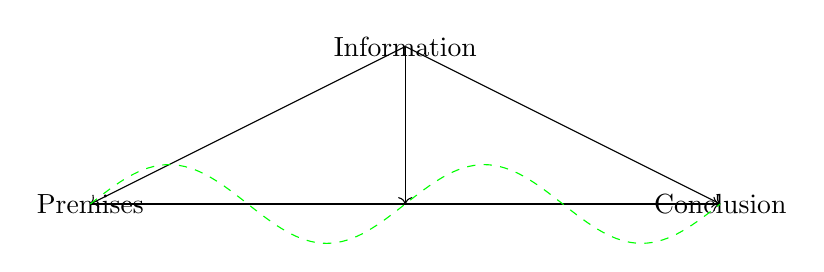
\begin{tikzpicture}
    \def\iHeight{2}
    \node at (4,\iHeight) {Information};
    \node at (0,0) {Premises};
    \node at (8,0) {Conclusion};
    \draw[->] (0,0) -- (8,0);
    \draw[->] (4,\iHeight) -- (8,0);
    \draw[->] (4,\iHeight) -- (0,0);
    \draw[->] (4,\iHeight) -- (4,0);
    \draw[green, dashed] (0,0) sin (1,.5) cos (2,0) sin (3,-.5) cos (4,0) sin (5,.5) cos (6,0) sin (7,-.5) cos (8,0);
  \end{tikzpicture}
  \caption{Sketch}
\end{figure}

\begin{note}[Expand tracking example]
  Consider tracking example.
  Here, on the relevant interpretation, the information provided to the novice allowed the novice to establish support relation.
  Understood here as providing information about to establish an appropriate connexion.
  And, given this information the novice goes ahead and establishes the (appropriate) connexion.

  Vary the example a little.
  Suppose the novice is provided with a book containing the information provided by the informer.
  Given understanding of base case, understand that the book is going to detail how to establish an appropriate connexion.
  Then, the novice reads the book, and fills in the detail.

  After reading the book, agent has doxastic support.

  Before reading the book, a more complex attitude.
  Conclusion on the basis of propositional support the novice has, and the result of establishing an (appropriate) connexion via the relevant contents of the book.
\end{note}

\begin{note}[Avoids problematic example]
  See how a problematic variant of the tracking example is avoided.
  Holmes and Watson.
  Holmes deduces, Watson looks on.
  This is one of those logic puzzles.
  It's the knave, or whatever.
  If it was just propositional support, then we'd be in some trouble.
  However, it's also the possibility of obtaining doxastic support.
  Watson lacks this, so don't get to claim.

  By contrast, if equals, then (Sherlock's brother) could claim, as they've observed Holmes and may do the reasoning.

  Maybe improve in which there's some initial evidence that one of the knights/knaves is untrustworthy, e.g. a criminal record.
  So, Watson would be fine believing this, that's all the evidence they have, without additional testimony.
  However, the brother couldn't.
\end{note}

\begin{note}[New example]
  Consider an abbreviated proof.
  Look at the premises and conclusion.
  So, have propositional support.
  Quite tired, so fail to see how the conclusion is obtained from premises.

  On the one hand, this has been reviewed, etc.\ so route to doxastic support.
  However, given understanding of material, then after some sleep and a cup of coffee, you'll recreate the reasoning in detail.

  Hence, hold the conclusion on the basis of premises, with a \future{} representing the appropriate connexion to be filled in.
\end{note}

\begin{note}[Existential]
  Support is flowing from the premises to the conclusion.
  It is not from ability.

  Difference is clearest when considering the instance of \AR{} in which the agent appealed to the attribute of having propositional support for the conclusion.
  In the case of \AR{} the agent appeals to having \emph{propositional support for the conclusion}.

  Here, the agent is appealing to \emph{that} propositional support, and `acceptance' that the propositional support leads to the conclusion.

  Subtle difference between appealing to the proposition that one has support for \(\phi\) and appealing to \(\psi\) which in turn supports \(\phi\).
\end{note}

\begin{note}[Contrast with \ref{denied-claim}]
  Noted that \ref{denied-claim} is understood with respect to doxastic, and here's where the incompatibility comes in.
  For, \ref{denied-claim} holds that a \future{} is no good.
\end{note}

\begin{note}[Key difference]
  The key difference between \AR{} and \WR{} is that with \WR{} the agent does not rely on ability/potential event for support.
  Rather, the agent relies on the support that they have for the premises which is independent of the ability information.

  Information in \WR{} does not --- and is not used to --- support the conclusion.
  Rather, it is the propositional support the agent has that does the work.
\end{note}

\begin{note}[Main motivation]
  Before turning to difficulties, there are a handful of things to say in favour of the first pass.
  Notably, that it provides a fairly clean expression of the core idea of \WR{}.
  Reducing to propositional support allows agent to appeal to reasons in support that they have not used.
  This is to some extend captured by propositional support.

  Two main sticking points.
  \begin{itemize}
  \item Weak attitude to relation between premises and conclusion --- one may require more.
  \item That the agent takes the propositional support to do the work.
    There remains some room to argue that the attitude toward propositional support for premises and attitude toward information are key.
    
  \end{itemize}
\end{note}

\subsubsection{Difficulty with first pass}
\label{sec:diff-with-first}

\begin{note}[Overview]
  The first pass assumed something about propositional support.
  That there is propositional support whether or not the agent does the reasoning.

  Whether or not agree with assumption, consider a pair of contrasting accounts of propositional support, and see how this assumption is important.

  After so doing, consider whether we can avoid assumption made.
\end{note}

\begin{note}[Different view of propositional]
  For example, \citeauthor{Turri:2010aa} argues for~\ref{Turri:PJ}.
  \begin{quote}
    \begin{enumerate}[label=(\textbf{PJ}), ref=(\textbf{PJ})]
    \item\label{Turri:PJ} Necessarily, for all \emph{S}, \emph{p}, and \emph{t}, if \emph{p} is propositionally justified for \emph{S} at \emph{t}, then p\emph{} is propositionally justified for \emph{S} at \emph{t} \textsc{because} \emph{S} currently possesses at least one means of coming to believe \emph{p} such that, were \emph{S} to believe \emph{p} in one of those ways, \emph{S}'s belief would thereby be doxastically justified.
    \end{enumerate}
  \end{quote}
  If so, then the availability of propositional support is secured by the potential event of reasoning.
  Hence, it seems that this reduces to a case of \AR{}.
  For, if the agent does not appeal to support for witnessing event, then the agent does not have grounds for holding that they have support for conclusion.
  It is not sufficient to observe that the agent has support so long as information about potential holds.
  Instead, the potential is doing the work in providing the agent with propositional support.

  Of course, \citeauthor{Turri:2010aa} doesn't require that the agent be aware.
  But this doesn't solve the problem.
  The issue is that the two instances of support coincide.

  It's somewhat straightforward to recast (\emph{PJ}) as `because the agent has the ability'.
  Indeed, \citeauthor{Turri:2010aa} speculates that propositional support is governed by abilities.
  Though, the exact relation between \citeauthor{Turri:2010aa}'s constraints and are use of ability is unclear.
  At the very least, \citeauthor{Turri:2010aa}'s seems weaker, as we require a sufficient collection of preconditions to be satisfied.
\end{note}

\begin{note}[Note]
  The difficulty is that if \citeauthor{Turri:2010aa} is followed, then there's no support to do the work.
  This does not mean that the premises are unavailable.
  Instead, the premises are inert.
\end{note}

\begin{note}[Same from \citeauthor{Goldman:1979ui}]
  \citeauthor{Goldman:1979ui} proposes \emph{ex ante} justification.
  \begin{quote}
    Person \emph{S} is \emph{ex ante} justified in believing \emph{p} at \emph{t} if and only if there is a reliable belief forming operation available to \emph{S} which is such that if \emph{S} applied that operation to his total cognitive state at \emph{t}, \emph{S} would believe \emph{p} at \emph{t}-plus-delta (for a suitably small delta) and that belief would be \emph{ex post} justified.\nolinebreak
    \mbox{}\hfill\mbox{(\citeauthor[21]{Goldman:1979ui})}
  \end{quote}
  Note that \citeauthor{Goldman:1979ui} talks of the `total cognitive state' of the agent at \emph{t}-plus-delta.
  It seems clear that the cognitive state of the agent at \emph{t} is relevant on in so far as the delta in \emph{t}-plus-delta is suitably small.
\end{note}

\begin{note}[Example?]
  However, following present line of thought, propositional support is a derived relation.
  It is a relation derived from some `attribute'.

  Clearest to see by recalling reasoning above.
  Project from event.
\end{note}

\begin{note}[Basic point]
  The observation here is that these accounts may taken as trouble for \WR{}, and in turn as partial support for \AR{}.
  Partial support for \AR{} as these accounts of propositional support are of propositional rather than doxastic support, and \AR{} is concerned with doxastic support.
  So, need to be furnished to show that an agent has the option of obtaining support for the conclusion of the reasoning that they are able to perform.

  It seems rather that this is an objection to the basic idea of \WR{}.
\end{note}

\begin{note}[This is trouble from \WR{}/Something about evidential relations]
  Not that these come easy.

  Basic understanding of propositional support.
  Seems support is a relation between premises and conclusion, or base and proposition.

  Common to talk in terms of `\emph{p} is propositional justified for \emph{S}'.
  Here, though, expanded.
  Sufficient reasons to believe that \emph{p}, and \emph{S} has those reasons.

  And, \textcite{Silva:2020aa} highlights troubles with evidential relations, and epistemic reasons.

  Similarly, because \emph{S} has ability, \emph{S} ought not to hold that \dots
\end{note}

\begin{note}[Bracketing possible issue]
  A possible lesson to be drawn from \citeauthor{Goldman:1979ui} is that there is no clear relation of support between premises and conclusion.
  Don't make sense to subdivide the agent's total cognitive state, or separate the means by which the agent may come to believe \emph{p}.

  This is the foundation of a challenge to~\USE{}.

  However, this isn't too much of a concern.
  Important for our purposes is preconditions.
  Talk of premises, is intuitive, what we're after, though, is some way of obtaining support which doesn't reduce to \AR{}.
\end{note}

{
  \begin{note}[The problem]
    The problem here is somewhat difficult.
    Following \citeauthor{Turri:2010aa}, it is the case that the agent has propositional support.
    However, the issue is whether the agent has the option of using the propositional support in order to obtain a kind of doxastic support.
    And, arguably this would lead to some conflict with~\nI{}.

    However, this isn't quite right.
    For, the relevant issue was that the agent isn't able to obtain support from general ability.
    This doesn't prevent the agent obtaining support from propositional support that's granted.

    Still, there does seem to be an issue.
    For, with the first pass, the agent has propositional support whether or not they have doxastic support.
    The basis for propositional support is general ability + potentive entailment.

    Here, why does the agent have propositional support?
    There's a witnessing event.
    Is the agent is a position to hold that they have propositional support?
    Well, the agent isn't in a position to use ability as a step in support.
    Seems like a conflict with~\nI{}.

    The difference is that the propositional support doesn't depend on the agent doing anything.
    This is a difference with \AR{}.
    For, with \AR{} the agent is using whatever support they have for ability.
    Here, ability grants propositional support.

    Basic point
    \begin{itemize}
    \item These accounts of propositional support mirror \AR{}.
      The difference is that \AR{} deals with a sort of doxastic support, while these concern propositional support.
    \end{itemize}
    And the first pass

    It's like, there's some doxastic support for propositional support.
    Isn't this at the core of the first pass?
    This does create some difficulty, as there's a way if the agent relies on general ability, but not if specific ability is required.

    Built in to the first pass is the idea that the agent has a good relation to the basis.
    If the relation of support is independent of doxastic support, then there's a fairly straightforward account of why this is the case.
    For, the agent has good doxastic support for their general ability, whatever that amounts to.
  \end{note}

  \begin{note}[Still thinking]
    Core idea is that on the first pass, the agent doesn't need any additional information in order for the premises to be propositional support for \(\phi\).
    Whatever it is that `directs' the propositional support is something other than the reasoning that the agent is able to perform.

    This is not so on G\&T.
    For, on G\&T, the propositional support to be propositional support for the conclusion, there's an additional component of what may be done with the support/premises.

    Either way, the agent doesn't have access to something that establishes that the premises are propositional support for the conclusion.
    The difference is whether or not this matters?

    Information about entailment, agent doesn't obtain support for this.
    However, the agent doesn't require support, on the basic understanding.
    There's no further aspect to propositional support before the availability of the relevant epistemic reasons.

    The agent doesn't have support that these are sufficient epistemic reasons for \(\phi\).

    So, granting entailment, have propositional support.
    Fits in the sort of prop -> conclusion schema.

    However, with G\&T, propositional support only by granting entailment.

    The entailment, and that there's ability, is required to get propositional support.
  \end{note}
}

{
  \color{green}
  \begin{note}[Developing the objection]
    This doesn't show there's anything particularly problematic with the first pass.
    It requires a particular understanding of propositional support, but so long as G\&T isn't true, then there's no problem.

    This is something of a technicality.
    For sure, this works.
    And, there's something of an argument for why G\&T don't hold up.
    For G\&T would require the agent to obtain support for ability.

    However, there's no argument for the understanding of propositional support unless the first pass is unique.

    Provides a solution which is somewhat consistent, but that's about it.

    Further, G\&T are in line with the basic idea.
    That is, propositional support in the same way that the agent seems to get support.
    The issue is that we're arguing that the agent has some access to the propositional support.
    So, it's a constraint motivated by a solution adopted without additional argument for why that solution needs to be adopted.

    The issue, then, is that this isn't illuminating.
    Fit various pieces together, but there's no clear understanding of why it makes sense to fit the pieces together in this way.

    This might be all that one could hope for, but perhaps we can do better.
  \end{note}
}

\begin{note}[Summarising]
  These issues with the first pass do not suggest that the first pass is false.
  Rather, the methodological concerns raised suggest that the reasons are somewhat lacking.
  If you're convinced, then go ahead --- I think there is something to be said.
  The second pass will be compatible with, but independent of, the first.
  Revisit this after the second pass is complete.
\end{note}

\subsubsection{Second pass: \future{} support}
\label{sec:second-pass:-futures}

\begin{note}[Following from problem]
  Noted G\&T.

  For, the potential event does the relevant work.
  With G\&T, this is used to identify propositional support.

  Raised a direct problem from first pass.
  In short, due to constraints imposed, agent isn't in a position to hold that they have support for conclusion.
  Led to a broader criticism of the first pass.

  Core insight of G\&T, though, is that witnessing may be put to work.
  As seen {\color{red} need to add} there's no way to figure out how the proposals really work without looking at potential events.
  At least for \citeauthor{Turri:2010aa}, the main claim is the priority of doxastic support.

  Question is whether there's a variation of G\&T where information from potentive entailment allows the agent to (`directly') claim support/base\dots
\end{note}

\begin{note}[Difference to G\&T]
  Start with differences\dots as these are important for the proposal.

  Difference between current case and G\&T is information about potential event.

  Suggest that this allows agent to defer reasoning while obtaining support.

  Allows the agent to form an attitude toward the conclusion, such that witnessing event in which agent establishes support is \emph{deferred}.
\end{note}

\begin{note}[Deferring]
  So, the intuition here is that one takes a standard case of reasoning.
  Two things.
  Claiming a basing relation.
  Establishing the basing relation.

  Often come together.
  Separate these.

  View as two different tasks.
  Understood this way, these tasks may be separated.

  Agent claims a basing relation and defers establishing.\nolinebreak
  \footnote{
    Note here on other use of deferring.
    Used when talking about infinitivism.
    Common idea, but the current interest is compatible with finitism/well-foundedness.
  }
  Information is used to maintain that establishing is deferred.
  (And not, for example, wished for.)

  Issue here is support.

  Basic motivation is that so long as the agent has the resources, then so long as the agent appeals to those resources, the agent obtains support (of a kind).
  This is in keeping with the first pass.
  Difference is that we don't reduce to resources (this is roughly how propositional support is understood).
  Rather, whatever those resources are, support is understood in terms of deference.
  Support is just what would be witnessed.

  In a slogan, the agent defers, rather than refers to that support.

  Agent defers.
  Introduce an intermediary.
  A \future{}.
  \future{} does the job of supporting conclusion.
  Does this job by being a placeholder, in effect.
  Unique thing about a future is that it doesn't matter when the details are filled in.
  Does the job of providing support because there's a guarantee that it may be filled in.

  Important here is that the guarantee that it may be filled in is not the source of support.
  The guarantee allows things to work/for this to be permissible.

  Agent sets up \future{}, takes support, defers establishing.

  Understand the support provided from an external perspective by filling it in.
  Here, parallel to G\&T.

  In relation to G\&T, the distinction is in the agent appealing to the same thing as what provides them with propositional support.
  Similar to the first pass, amounts to the agent obtaining support for propositional support, roughly.
  However, here, the support for propositional support is just the source of propositional support.

  Key, again, is that the agent is not appeal to support they have that there is such a potential event.
  Rather, the agent is appealing to the relation of support that would be established by witnessing the potential event.

  This is the understanding of deferral.

  Intuition for why this provides support is that it is in certain respects functionally equivalent to propositional support.
  One both accounts of propositional support, agent has support.
  Common way of understanding things.

  Agent defers transforming that propositional support into doxastic support.
  However, that the agent is so deferring allows the agent to appeal.
  Here, it is the deference that is doing the work.
  If called for, then provide the relevant support.

  The idea, then, is that deferred support functions in the suitably similar ways.
  It is a \emph{kind} of support that the agent may appeal to.
  Prefixing an adjective is difficult.
  Fake passport won't let someone board a plane.
  Likewise for corrected typogrophical mistake.
  Small elephant is an elephant, and Deferred compensation is compensation.
\end{note}


\begin{note}[Examples of deferring]
  Separation of this kind of common.
  For example, purchasing and paying.
  Purchase a car, but with a loan.
  Have not, in some sense, payed for the car.

  With the loan analogy, so kind of guarantee is typically required.
  Analogy extends in this respect.
  Agent needs some kind of guarantee that they may establish support.
  This is the role of the information.

  As noted, the agent is in a position to use the information, but not derive support from the information.
  Here, the agent uses the information to set up a relation of support, and the information simultaneously functions as a guarantee for deferred establishment, or filling in.

  Deferred shipment?

  Another example is with language.
  Referring term, but assigning reference is deferred.
  Not sure how to design an example, though.
\end{note}


\begin{note}[After examples]
  Key idea, then, is that relation is created, witnessing is deferred.

  First pass, primary worry was that it wasn't particularly illuminating.
  It seems to me that second pass fares better.
  See the information as providing a guarantee.
  Motivated by understanding what the information (if true) entails.

  Independent of any particular account of propositional support.
  In contrast to the first pass, then, the agent is not appealing to support that they already have for propositional support, so to speak.
  Idea of propositional support continues to inform understanding of the support the agent has, but this is because the two kinds of support share the common feature that the agent has not witnessed any demonstration.

  First pass relied on this idea that the agent was in a position to form a belief that they had propositional support.
  Here, what is doing the work is the opportunity to provide (doxastic) support.

  What we miss from the first pass is an argument (assuming information is true) that the agent has propositional support.
  However, we retain an account of why it makes (at least some) sense for the agent to claim support.

  One may continue to hold that independent propositional support has a role, and is part of the explanation.
  For example, some story about support having propositional support.
  However, this is a non-essential component of the proposal.

  A \future{} is a kind of token that the agent may point to, whose availability is governed by sufficient guarantee.
  And, this provides a kind of support.
\end{note}

\begin{note}[Novelty]
  The novelty of the proposal is \dots

  the split between claiming and establishing, and deferring establishing
  support

  The split simply requires developing (conceptual) vocabulary.
  Nothing in particular follows from deferring if it never occurs.
  Support is the substantive component.
  Certain things do follow.
  However, by itself there is no incompatiblity with~\ESU{}.
  The incompatiblity arises from application to these cases.

  Useful observation, as can introduce concepts with compatible examples.
  Do so with the problem of forgotten evidence.
  Offers some useful distinctions and predictions.

  Turn to extending into the future.
  So long as we've been careful, this doesn't follow from anything claimed.
  However, closed the gap.
\end{note}

\begin{note}[Figures]
  \begin{figure}[h]
    \begin{subfigure}{.5\textwidth}
      \centering
      \begin{tikzpicture}[->, >=stealth', node distance=0cm, every text node part/.style={align=center}]
        \node [] (c) at (0,0) {};
        \node [] (d) at (-3,0) {};
        \node [] (e) at (3,0) {};
        \node [] (f) at (0,-2.1) {};

        \node (A) at (0,-.1) {P};
        \node (C) at (0,-2) {C};

        \draw [->, xshift=4] (0,-.35) to  node[right] {} (0,-1.75);
      \end{tikzpicture}
      \caption{\AR{}}
    \end{subfigure}
    % \hfill
    \begin{subfigure}{.5\textwidth}
      \centering
      \begin{tikzpicture}[>=stealth', node distance=0cm, every text node part/.style={align=center}]
        \node [] (c) at (0,0) {};
        \node [] (d) at (-3,0) {};
        \node [] (e) at (3,0) {};
        \node [] (f) at (0,-2.1) {};

        \node (A) at (0,-.1) {P};
        \node (C) at (0,-2) {C};

        \draw (-.1,-1.8) -- (-.3,-1.8) -- (-.3,0) -- (.3,0) -- (.3,-1.8) -- (.1,-1.8);

        \draw [->, xshift=4] (0,-.35) to  node[right] {} (0,-1.75);
      \end{tikzpicture}
      \caption{\WR{}}
    \end{subfigure}
    \caption{Relations of support for \AR{} and \WR{}}
  \end{figure}
\end{note}


\begin{note}
  First part.
  Reasoning as a function.
  Allows one to abstract and introduce a \future{}.

  \future{} gets paired with a potential.
  Fulfil \future{} just in case true that potential.

  Introduced in terms of our use case.
  Fairly general.
  Use from premises instead.

  Parallel to quantifiers.
  Here, get truth of existential by possibility of updating assignment function where \(x\) is turned into a constant, effectively.
  Could also take a distinct understanding of a variable.
  Benefits to having two quantifiers, but quite possible to rewrite rules in this way.
  Interpretation where \(x\) is something between a variable and a constant.

  \future{} works the same, but slightly more complex.
  \future{} is introduced with background potential.
  Then, updated when potential is witnessed.

\end{note}




\hozlinedash{}

\begin{note}[\future{}]
  Suggestion is to introduce idea of a \future{}.

  Understanding of doxastic support is appropriate connexion.
  Information about ability means that appropriate connexion may be established.
  A \future{} stands in place of the relation, it fixes that the attitude is connected to premises, etc.
  So, whatever the appropriate connexion would be, any resolution of the \future{} will satisfy that connexion, and the information about ability (in part) allows the agent to be confident that they may fulfil the \future{}.
\end{note}

\hozline{}


\begin{note}[Starting out the problem of forgotten evidence]
  Goldman's Problem of Forgotten Evidence.

  \begin{quote}
    Many justified beliefs are ones for which an agent once had adequate evidence that she subsequently forgot. At the time of epistemic appraisal, she no longer possesses adequate evidence that is retrievable from memory.
  \end{quote}

  Here, interest in the problem is for what \citeauthor{Goldman:2011vn} terms `preservative memory':
  \begin{quote}
    Preservative memory does not create or generate justifiedness `from scratch', but instead transmits a belief's justifiedness (or unjustifiedness) from one time to a later time.\nolinebreak
    \mbox{}\hfill\mbox{(\citeyear[259--260]{Goldman:2011vn})}
  \end{quote}
  Time shifted instance of cases we're interested in, where agent has done the reasoning at some point in the past, and has information about result of reasoning on this basis.

  \begin{quote}
    People frequently fail to recall their original sources of evidence for things they know or justifiably believe.
    First, they often don’t have memory-based beliefs about their original sources.
    [Second] they rarely have memory experiences of specific perceptual episodes (what psychologists call `episodic' memories) in which they were exposed to relevant observational evidence.
    It is extremely implausible to claim that for every moment at which a justified belief is stored in your mind, you undergo an episodic memory experience of one or more past (perceptual) experiences that constituted your evidence.\nolinebreak
    \mbox{}\hfill\mbox{(\citeyear[266--267]{Goldman:2011vn})}
  \end{quote}

  Here, preservative memory transmits.
  Example of way I'm understanding this by a conditional.
  Takes a lot of steps to reason from A to B.
  \(A \rightarrow B\) as a preservative memory.

  Goldman presents this against (particular kind of) internalism.
  But this isn't quite right.
  Particular kind of internalism.
  It may be that all internalists hold this synchronosity requirement, but I'm not clear on why this needs to be the case.
  Not so much our interest.
  \cite{Korcz:2019tl} sketches out the general response from internalist lines.

  Of interest here is that this remains compatible with the basic idea of epistemic debt.
  Remains clear that the agent requires resources to re-establish the relevant beliefs.
  So, we're not assuming anything strong.

  Perhaps better to frame this as forgotten basis.
\end{note}

\begin{note}[Substantial premise?]
  The substantial premise here is that evidence of interest may go beyond what one has at a particular time.
  This is substantial, but consistent with~\ESU{}.
  So, granting this does not sneak in an assumption against~\ESU{}.
\end{note}

\begin{note}[Example: Lost]
  Running.
  Note down times in a book.
  End of year, note fastest time.
  Form belief.
  Accuracy of notebook.
  Time passes, remember speed, but have forgotten evidence.
  No way to recover evidence.

  Might still hold memory does the job, clear this is a different basis.
\end{note}

\begin{note}[Example: Regained]
  Proving theorem.
  Write down.
  Hold theorem to be true.
  Forget proof.
  Paper is destroyed.
  Need to reprove.

  Here, there's something to be done.
  Problem to be solved like any other, but understand what the solution is.
  And, measure of the resources required.
\end{note}

\begin{note}[~\ESU{}]
  The kind of considerations here are compatible with~\ESU{}, as the agent has (at some point in the past) reasoned from premises to conclusion.
\end{note}

\begin{note}[Difference between scenarios?]
  Built in difference between these two cases.
  Does this make a difference to support?

  It seems there is some difference.
  Going via `why' questions.
  Suspect that it is plausible that one need answer with memory in the first, but not the second.
  Indeed, seems puzzling for the second.
  Returns to what is now a running theme, which is that proofs don't seem to work if testimony is required.
  Hence, if I'm relying on memory, seems analogous to testimony, and it doesn't seem I can hold on the basis of a premises (and proof).
  
\end{note}



\begin{note}[Coffee]
  First observation is that there's an understanding of work to be done.
  Second is that in the memory case, the agent has information about what that work would be.

  Add to this the idea that the agent retains support.

  On \citeauthor{Goldman:2011vn}'s view, this is because preservative memory is `a cognitive belief-retaining process that is able to transmit justifiedness from an earlier to a later time' (\citeyear[261]{Goldman:2011vn}).
  Here, original evidence does the work.

  However, additional observation is that the agent has the resources to (re-)establish.
  Or, there is a potentive event in which agent establishes \dots
  This provides a distinction between the two cases.

  Further, we find a difference between a difficult case.

  This is the coffee addict.

  To the extent Joe would do well when (re)establishing, it seems we're good.

  Here we do get something different from the first pass.
  For, propositional support would remain the same.
  Instead, it's that the potential reasoning would work out well given revisions to Joe that does the work.
  This isn't accounted for by the presence of propositional support.
\end{note}


\begin{note}[Sketch]
  Provides some understanding of what is at issue.
  Epistemic debt, in the sense of resources required to (re)base theorem.
  To what extent this matters, in general, is a distinct question.
  Terminology may seem leading, but memory is derivative in these types of cases.
  Something else is doing the work.

  Important, in the sense that proposition is held on some basis.
  

\end{note}



{
  \color{red}
  \begin{note}[Intuition: messages]
    Intuitive way to understand is in terms of messages.
    The agent creates an envelope with an address to the relation of support.
    This envelope is passed forward.
    At some point, when the agent has the time or resources, the agent establishes the relation of support.
    This information is written down, placed in the envelope, and is sent.

    Want to send the letter.
  \end{note}

  \begin{note}[Card example]
    Give receiver a card, no funds.
    Receiver won't use the card before \(t\).
    Add funds before \(t\).

    But this just is a credit card, in a sense.
    Pay now, with security of salary arriving before credit needs to be paid.

    So, this is debt, or a promise.
  \end{note}
}

{
  \begin{note}[Notes]
    On the revised version of the first pass (to be completed) there is no need to deal with the idea of a \future{}, as witnessing is there to explain the way in which the `entailment' works.
    The second pass, then, is where the idea of a \future{} is introduced.

    The agent is not extending propositional support that is already available to the agent.
    Instead, we've got something that's really asynchronous.
  \end{note}

}

\begin{note}[Is this only surface deep?]
  Introduced the idea of a \future{}.
  Allowed an agent to establish doxastic support on basis of `pre-existing' propositional support.

  The primary problem with the first pass in terms of propositional support stems from the possibilities of reducing propositional support to doxastic support.
  Hence, if reduction, then the understanding of \WR{} in terms of propositional support reduces to an instance of \AR{} --- support for premises that the agent appeals to just is the support the agent has for ability, or potential event in which agent witness the relevant action.

  Due to role of propositional support, then, any variation on the basic idea will inherit this issue.
  Tentatively, then, \WR{} requires a particular understanding of propositional support.

  Note, this is only a problem for one part of the first pass.
  Do not have the option of relying on pre-existing support relation.

  That the premises must stand in an existing support relation may be challenged.

  We have already seen that it is plausible that any support obtained prior to witnessing the reasoning is distinct from the support that would be obtain by witnessing the reasoning.

  Suggestion is that support flows through `\future{}' relation of support.
  Avoids propositional support.
  Additional benefits.
\end{note}

\begin{note}[Support]
  Well, the point here is that the support relation may be considered with an reference that has not yet been fixed.

  So, instead of taking a `pre-existing' support relation, as in the case of propositional support, obtain support because the support established in potential event may be `brought forward' by establishing premises and relation whose referent is `deferred'.

  The novelty here is that support transmits through `deferred' support.
\end{note}

\begin{note}[Asynchronous]
  Intuitively, this is asynchronous.
  The agent establishes relation of support given information.
  Then, at some other times details exactly what the relation of support is.
  The unique thing in these cases is that the agent has information about what the result of the deferred detailing is, and thus has the option of establishing a relation of support to be filled in.

  Always in terms of potential witnessing event.
  Information the agent has grants witnessing event.
  Preserved under variation of premises, so long as potential event remains.

  Contrast to propositional support, which did not require anything asynchronous.
\end{note}

\begin{note}[Promises]
  Introduced in \textcite{Liskov:1988vo}.
  Decouple process of establishing relation support, and detailed what the relation of support is.

  Information that the agent has the ability, or that there is a potential event, is used to create a promise.
  However, support is distinct from this.
\end{note}

\begin{note}[The really important thing]
  Support is flowing from the premises to the conclusion.
  It is not from ability.

  If propositional support that does not reduce to ability, then no need to take this as a primitive.
  If not, then perhaps.
\end{note}

\begin{note}[Why does the agent obtain support?]
  A \future{} is something of a primitive.
  And support is very general.
  So, not really possible to work from some more basic premises.

  Instead, consider it a hybrid of the two types of propositional support considered.
  Like general propositional support, holds whether or not agent has done reasoning.
  Like \citeauthor{Goldman:1979ui} etc.\ potential events inform.

  Not assuming propositional support.
  Or, assuming that information about potential event may not provide information about pre-existing relation of support.
  So, where does support come from?

  Well, we've got a \future{}.
  Associated promise.
  The promise is not providing support.

  What is added is specification of how agent obtains support for conclusion.

  The potential event, then, ensures that support may be obtained.

  Support for conclusion because potential event provides sufficient information guarantee relation of support may be established.
  What remains is fixing the specifics.

  The support for the conclusion just is the support that the agent would obtain from witnessing.
  The thing is that the reasoning part is the only thing that's missing.
  It's the details that are deferred.
  I.e.\ asynchronous.

  Illustration with standard case, then cutting a pasting for a different temporal order.
\end{note}

\begin{note}[Different from strategies/plans]
  With a \future{} comes a potential event, something to be done.
  However, this is distinct from a strategy or a plan, which is a representation of something to be done.
  That is, a \future{} is \emph{not} a plan.
  A \future{} is simply a placeholder.
\end{note}

\begin{note}[Social parallels]
  Relationship between inter-personal and intra-personal agency.

  Difficulty with inter-personal as testimony.
  However, have noted from \citeauthor{Easwaran:2009tm} that certain cases information about entailment and support come apart.

  This relates to `buck-passing' (\citeyear{Baker:2018aa})
  \textcite{Baker:2018aa} suggest `strong buck-passing'

  \begin{quote}
    \textbf{Strong B-P:} When challenged to produce the evidence that justifies her belief that p, A can acknowledge that she is unable to do so by herself, without help from her source, without thereby undermining her claim to know that p.\nolinebreak
    \mbox{}\hfill\mbox{(\citeyear[8]{Baker:2018aa})}
  \end{quote}
  \citeauthor{Baker:2018aa} don't directly argue for strong buck-passing.
  Instead, suggest that it has certain advantages given independent commitments regarding testimony.

  Kind of considerations that motivate \citeauthor{Easwaran:2009tm}'s view on transferability suggest plausibility of buck-passing.
  Place as intermediary between two skilled mathematicians.
  Intermediary will pass the buck to presenter when questioned by agent.
  For, proof is transferable.
  And, intuitively does so because testimony is not required.

  The agent then doesn't seem to be in the same position.
\end{note}

\begin{note}[Other cases]
  Thinking back to the tracking case may be helpful.
  In the case, information allowed the agent to establish (doxastic) relation of support.

  If propositional support doesn't work as expected, then prior the agent did not have propositional support.
  (This is a plausible reading of \citeauthor{Turri:2010aa}'s remarks on the more fundamental stuff that goes on with support, though could be avoided.)

  The difference is that the information is restricted in the case of interest.
  But the \future{} \emph{functions} in an analogous way.
  It just doesn't carry (sufficient) information about the relation.
\end{note}


\begin{note}[How support works]
  In the case of reasoning, the result will be that the agent has information about premises.
  Here, it is important to note that the agent has `propositional' support for the premises, independent of the ability information.
  So, the agent does not need to appeal to the existence of the event as a premise in obtaining support for the conclusion.
  The only relevant support the agent has is the support for the premises.
\end{note}

\begin{note}[Similar applications of the basic idea]
  Introduce idea that this is something of a placeholder.
  Perhaps use the example from names with an as yet unidentified reference to provide additional motivation.

  The idea is similar in principle.
  There is someone out there in the world.
  Just as there is support that the agent may use.
  So, the remaining task is to fix the interpretation of the name.
  Likewise, the remaining task for the agent is to witness the relation of support.

  In both cases, establishing the additional stuff is useful.
  Foremost, resolves the possibility that the `\future{}' may not be resolved.
  And, other minor benefits in terms of further information.
\end{note}

\begin{note}[Giving up on synchronous support]
  This is something of a cost.
  Cost captured in large part by~\ESU{}.

  Difficult.
  For, if basic understanding of propositional support, then still require something to explain how the agent transforms this to doxastic support.

  Still, two plausible pictures.
  Pre-existing propositional support.
  Support obtained through use of a \future{}.
\end{note}

\begin{note}[Upshot]
  Main upshot is relation of support.

  One nice upshot is that there is a clear link between the support obtained prior to reasoning, and the support obtained by reasoning.
  It's filling in the deferred reasoning.

  May expand.
  For example, with a promise to resolve the support relation.

  Another upshot is that ???
\end{note}


\subsubsection{Generating potentive inference and \future{}}
\label{sec:generaling-future}

\begin{note}[Idea]
  Here, setting up for weakness of will.
  Idea is that second pass doesn't require the agent to `have' support already.
  This means that one may take a generalisation of potentive inference which allows for some incoming information, etc. and apply the idea of a \future{} to get something much more general, so long as the relevant guarantee is in place.
\end{note}


\subsection{Distinction between \AR{} and \WR{}}
\label{sec:dist-betw-ar}

\begin{note}[Overview]
  The important difference is what supports the conclusion.

  Here, we suggest that further differences depend on additional commitments.
\end{note}


\begin{note}[Key Issue]
  The key issue is whether the agent obtains support for all the relevant preconditions of witnessing the ability by witnessing.
  And, whatever follows from this, e.g.\ in terms of commitments and so on.

  If so, then anything that follows from \AR{} also follows from \WR{}.
  Conversely, as the agent does not obtain information about how the ability is witnessed, it seems what follows from \WR{} also follows from \AR{}.
\end{note}

\begin{note}[Interesting case]
  Interesting case to think about, in which the agent obtains support for what follows from witnessing, but intuitively not for some other precondition.
  \begin{itemize}
  \item Ability to reason to \(\phi\).
  \end{itemize}
  Entailment applies to \(\phi\).
  Entailment doesn't seem to apply to reasoning to \(\lnot\phi\) as misleading.
\end{note}

Understanding of ability is such that there is always a potential witnessing event.

\ESU{} and~\nI{} are universal claims.
\ref{prop:SE} is an existential claim.
\ESU{} and~\nI{} clash in scenarios where the possibility captured in~\ref{prop:SE} is realised.

The collection of~\ESU{},~\nI{}, and~\eA{} is in tension.

There is an additional secondary premise:

\begin{note}[Two ways to understand ability and support]
\begin{enumerate}
\item\label{prem:ability} Two ways to obtain conclusion given ability.
  \begin{enumerate}
  \item Attribution.
  \item Witnessing.
  \end{enumerate}
\end{enumerate}

\ref{prem:ability} does not make a claim about any particular use of ability.
As a template, conceptually (or logically) coherent.
If there's a problem, then it's because there are further constraints on understanding of support.
\end{note}

\section{Miscellaneous}
\label{sec:misc}

\subsection{Metabelief}
\label{sec:metabelief}

\begin{note}[Idea]
  A possible solution I've overlooked is the idea of some belief of the form of a metabelief that if one has information about ability, then it's true.
  Something of a background belief.
  Put to work in various contexts.
  For example, testimony, problem of forgotten evidence, and so on.

  Somewhat close to induction, maybe?
\end{note}

\begin{note}[Reduction?]
  From a certain point of view this seems to be an instance of~\nI{}.

  I mean, the difficulty here is the way in which the agent gets to the information.
  That is, this kind of metabelief in a sense, provides exceptions to~\nI{}.

  I don't find this particularly plausible.
  In a sense, it works.
  So long as agent goes from truth to truth.
  But something more is needed.
  Understand that affirming the consequent is bad.
  However, when I use it, always find.
  So, form metabelief.

  Affirming is bad, regardless of use.
  Inclined to think the same is true here, and~\nI{} highlights why.
\end{note}

\subsection{\citeauthor{Audi:1983ux} on \citeauthor{Lehrer:1971aa}}
\label{sec:lehrer}

\begin{note}[Lehrer]
  \citeauthor{Lehrer:1971aa}'s cases are somewhat of interest.

  Here, we have an agent who seems to have both propositional some proposition.
  The propositional support is stipulated as unquestionably good, take this to be established however one likes.
  However, obtaining doxastic support is difficult, and the agent does not recognise that they have propositional support.
  Instead, the agent forms a contrary attitude based on contrary propositional support.

  So we have:
  \begin{enumerate}
  \item\label{L:gl:prop:p} Propositional support for \(\phi\)
  \item\label{L:gl:prop:not-p} Propositional support for \(\lnot\phi\)
  \end{enumerate}
  Were the support for \(\phi\) is stronger than the support for \(\lnot\phi\).
  And, the haven't has established doxastic support for \(\lnot\phi\).
  As the agent has not established doxastic support for \(\phi\) (due to difficulty), the agent believes \(\lnot\phi\).

  The agent then is then informed by some source that the agent has (stronger) propositional support for \(\phi\).
  The agent then goes and establishes doxastic support for \(\phi\).
  However, due to the complexities involved, the agent is not swayed by the doxastic support.
  For example, some errors.
  However, because the source provided information that propositional support is stronger, agent revises attitude in favour of \(\phi\).
\end{note}

\begin{note}[Example]
  \citeauthor{Lehrer:1971aa} specific example involves a questionable source, and it is unclear whether there's much to be said for the agent.

  Variant with student.
  Student attempts to prove something.
  It's quite difficult, and the agent's intuitive understanding of the domain guides them to \(\lnot\phi\).
  So, student has strong belief that \(\lnot\phi\) is the case, though lacks knowledge --- the student has not ruled out that \(\phi\) is the case.
  Teacher suggests that the material establishes \(\phi\).
  Student takes a second look, and following the formalism, proves that \(\phi\).
  However, the agent has no intuitive understanding (some of the) key steps in the proof.
  So, the agent relies on the teacher.
\end{note}

\begin{note}[Possible to read \citeauthor{Lehrer:1971aa}'s example as similar]
  If the agent obtains support for \(\phi\), then it seems this is due to the propositional support the agent has, rather than the doxastic support that the agent forms.
\end{note}

\begin{note}[\textcite{Audi:1983ux}]
  \citeauthor{Audi:1983ux} presents a neat summary of how the argument may go:
  \begin{quote}
    Since
    \begin{enumerate*}[label=(\arabic*)]
    \item\label{Audi:divergence:1} the justification of the belief that \emph{p} is \emph{q}, which is good evidence for \emph{p}, and
    \item\label{Audi:divergence:2} S believes \emph{q}, and sees its full evidential bearing on \emph{p},
    \item\label{Audi:divergence:3} S has good evidence for \emph{p}.
      Hence,
    \item\label{Audi:divergence:4} S has a justification for the belief that \emph{p}.
      Thus,
    \item\label{Audi:divergence:5} if S believes \emph{p}, then even if his believing \emph{p} is not to any degree sustained by his believing \emph{q}, he justifiably believes \emph{p}, and the (or a) justification of this belief is based on his belief that \emph{q}.
    \end{enumerate*}
    \nolinebreak
    \mbox{}\hfill\mbox{(\citeauthor[406]{Audi:1983ux})}
  \end{quote}
  \citeauthor{Audi:1983ux} suggests the argument falters from step~\ref{Audi:divergence:4} to~\ref{Audi:divergence:5}.
  In short, the agent doesn't get doxastic support from proposition support.
\end{note}

\begin{note}[Important difference]
  There is an important difference between the two types of cases.
  In the \citeauthor{Lehrer:1971aa} type cases, the agent discards the doxastic support.
  In our type of case, the agent has not yet obtained doxastic support (implicit has been that the agent would obtain doxastic support).

  So, in our cases, there is scope to reject~\ref{Audi:divergence:5}.
  Do need some kind of sustaining, and the use of information about ability establishes the relevant sustaining.
\end{note}

\begin{note}[Notes for the moment]
  Todo is to work through \citeauthor{Audi:1983ux} in some detail and see if there's a stronger argument against the position I endorse.

  A potentially important point is that there's no counterfactual dependency in \citeauthor{Lehrer:1971aa}'s cases, while there is some kind of counterfactual dependency in the cases of interest.

  Should check: \textcite{Tierney:2012tt}.
\end{note}


\subsection{Additional observations}
\label{sec:addit-observ}

\begin{note}[Trouble with modals]
  We have sketched potentive entailment.
  However, noting the interaction between a modal and a verb.

  Understanding of why the entailment works has been left largely to intuition.

  The specifics of potentive entailment are not too important, so we may omit the detour.
  Still, even for those willing to make the detour it is not clear how long it would take, or where it would lead.

  Difficulty is seen by taking a straightforward treatment of the modals involved.

  `There is potential for' and `agent S has the (specific) ability to' are modals.

  Standard first pass at modals, via possible worlds and accessibility relations.

  Before continuing further, the presence of difficulty may be quickly noted by noting the similarities between potentive and actuality entailments.
  \textcite{Alxatib:2019wf} provides the following account of actuality entailments.
  \begin{quote}
    Actuality Entailments (AEs) are inferences from premises that appear to be modal, like (1a), but their content is that the modality is effectuated in the evaluation world --- (1b).

    \begin{enumerate}[label=(\arabic*)]
    \item
      \begin{enumerate}[label=\alph*.]
      \item Pierre a dû \hspace{26pt} prendre le \hspace{3.5pt} train \newline
        Pierre had.to.\textsc{pfv} take \hspace{14pt} the train\newline
        \hspace{-4pt} ‘Pierre had to take the train'
      \item \emph{Inference}: Pierre took the train.\nolinebreak
    \mbox{}\hfill\mbox{(\citeyear[701]{Alxatib:2019wf})}
      \end{enumerate}
    \end{enumerate}
  \end{quote}

  Note, the reading of `had' in (1a) is `unambiguously deontic' (\citeyear[703]{Alxatib:2019wf}).
  English paraphrase does not carry the same entailment, but does seem to carry a corresponding implicature.

  Potentive entailment is related, but it is not (necessarily) the \emph{content} on the modality that is effectuated in the evaluation world (though it may be).
  Following the account of actuality entailments, \citeauthor{Alxatib:2019wf} highlights the basic problem:

  \begin{quote}
    AEs are surprising; if we assume that modals attribute their propositional argument to potentially non-actual worlds, something must be special to AE-licensers that leads to the inference of actuality.

    Whatever that special feature is, its effect is complex, and it interacts in nontrivial ways with other phenomena of theoretical interest.\nolinebreak
    \mbox{}\hfill\mbox{(\citeyear[701]{Alxatib:2019wf})}
  \end{quote}

  Possible world, then the event takes place in the possible world.
  Had takes some ordering, so best world involved taking the train.
  This doesn't seem to explain why Pierre took the train.

  Similar with potentive.
  There is a possible world, but it's not obvious why this constrains the world of evaluation.

  With examples, it is clear that there is an entailment.
  Substituting different verbs and results, entailment goes away.

  This isn't too helpful.
  For, we would see what is required to be the case at the possible world.
  However, the consequent of a potentive entailment holds at the world of evaluation.

  Of the form \(\Diamond \phi \rightarrow \psi\).
  So, \(\lnot \psi \rightarrow \Box \lnot \phi\).

  Potential clue.
  Restrictor.
  In effect, the potentive entailment is drawing out information about the restrictor/modal base.

  Figuring out the relevant construction of modal base \dots well \dots
  Something of a dead end.
\end{note}

\begin{note}[More on actuality entailment]
  The potentive entailment is not an actuality entailment.

  \begin{quote}
    \begin{enumerate}
    \item Yesterday, John was able to eat five apples in an hour. (past episodic)
    \item In those days, John was able to eat five apples in an hour. (past generic)
    \end{enumerate}
    (315a) implicates that John actually ate five apples in an hour.\nolinebreak
    \mbox{}\hfill\mbox{(\citeyear[173]{Bhatt:2008aa})}
  \end{quote}

  \begin{quote}
    (317) Last night, a masked assailant attacked me on my way home.
    I was able to wrestle him to the ground.
    \#But I didn't do anything since I am a pacifist.\nolinebreak
    \mbox{}\hfill\mbox{(\citeyear[174]{Bhatt:2008aa})}
  \end{quote}

  Key here is the entailment is restricted to the event, and the modal needs to be in the past tense.
  (\textcite{Pinon:2003te} has some nice examples.)
  Of course, potentive entailment applies.
  Certain conditions had to be in place in order for there to have been a witness of ability.
  Still, these seem to be distinct as they do not conform to the same restriction placed on actuality entailment.

  There is some work on the difficulties involved in obtaining the actuality entailment.
  \citeauthor{Bhatt:2008aa,Bhatt:1999ud} argues that the entailment doesn't follow from ability attribution.
\end{note}


\subsection{Agentive modals}
\label{sec:agentive-modals}

\begin{note}[Summary]
  This is something of an appendix to the present chapter.
  The goal is to review the literature on agentive modals, and highlight that there is some difficulty with obtaining a clear understanding of potentive entailment from the proposals made.
\end{note}

\begin{note}[Agentive modals]
  Agent is able to \dots

  Ability modal.

  \begin{enumerate}
  \item It is possible that Y stole the jewels.
  \item S has the ability to prove that Y stole the jewels.
  \end{enumerate}

  The ability statements of interest are an instance of agentive modality.
  \cite{Mandelkern:2017aa}
  \cite{Maier:2013vk}
  \cite{Schwarz:2020aa}
  \cite{Willer:2021ur}
  \cite{Maier:2021te}

  Some proposals, and some issues.
  E.g.\ Kratzer on `can'.
  The dart board problem.

  For the moment, leave the literature on ability modals aside.
  Focus is on specific ability.
  And, in particular, ability to reason.
  Literature focuses on non-mental actions.
  Throwing darts, unlocking safes, etc.
  In most cases the result of witnessing the ability depends on witnessing the ability.
  If the agent does not throw the dart, it will not land on the board.
  If the agent does not unlock the safe, then the safe will not be unlocked.

  Some further details in section~\ref{sec:agentive-modals}
\end{note}

\begin{note}[No volition]
  Tempting to restate in terms of volition.
  For example, paper.
  Presents some difficulty, especially given the observation that the agent may not at present have the volition.
  For, then to evaluate the entailment, need to consider some counterfactual possibility.

  S is able to prove that Y stole the jewels.

  This is because S is heavily involved.
  S has no volition to do so.
  This would result in estrangement for S.
  Without some complexity, it seems that in order to assume S has the volition, we would need to assume that S was not involved.
  Therefore, in turn, that the jewels were not stolen, or that the resulting proof would be different from what it actually is.
\end{note}

\begin{note}[Potentive entailment and modals]
  Given sufficient context, instances of the potentive entailment apply.
  There are darts available, there is a safe.

  Further, focusing on the modal aspect leads us to some difficulties.
  The entailment tells us about how things are in order for something to be possible.
  It is not clear how to conceptualise this.
  Consider possibility.
  In general, no potentive entailment.
  It is possible that the sun rises from the west.
  Unclear what follows about how things actually are from this.

  Properties of the accessibility relation?
\end{note}

\begin{note}[???]
  Doesn't rule out property.
  Don't get into the ontology of potential events.
  So, may reduce.
  Still, from the perspective of reasoning, not required.
  Entailment follows from potential, and potential may require attribution of ability, but only from some ontological perspective.
\end{note}


\section{Formal?}
\label{sec:formal}

\subsection{Obtaining potentive entailments}
\label{sec:obta-potent-enta}

\begin{note}[Quick sketch]
  This is an optional section.
  We explained potentive entailment and given examples.

  Reader may wish for a technical account.
  In this section we sketch one such account.

  We do not argue that the account is wholly adequate.
  However, functional at first pass.

  Two things to do.
  \begin{enumerate}
  \item Establish some equivalence between potential and ability.
  \item Given an account of the potentive entailment.
  \end{enumerate}

  Start by taking a simple possibility understanding of the modal and show how potential and ability fit.
  We will then build on the possibility understanding to fix potentive entailment.
\end{note}

\subsection{Modal}
\label{sec:modal}

\begin{note}[Potentive]
  The potentive is straightforward to analyse.

  Fairly clear understanding of event semantics.

  Here, existential quantification over events is replaced by a modal.

  This requires some non-standard existential, but we're not too interested in providing an analysis suitable for semantics.
\end{note}

\begin{note}[Ability]
  Our understanding of ability is basically the same as potentive.

  Ability functions as an equivalent quantifier.
\end{note}

\begin{note}[Avoid ability?]
  A simple corollary of the above observations potentive entailment does not require ability.

  If it is possible to provide information about potential event of reasoning without attributing ability, then we don't need to speak of ability at all, perhaps with the exception of generating intuitive scenarios.

  May wonder how important ability is.

  Difficult case.
  Go for externalism, and co-reference.
  State a conclusion, but the agent would not reason to the conclusion under that description.

  There's a potential event, but it isn't clear that the agent has the ability.

  Doubt this is possible, as agent needs to do something.
  And, ability this seems sufficient for an ability statement.
  So, continue to work with ability.
\end{note}

\begin{note}[Some formal stuff]
  \[(\text{Able}(s,e) \land (V(e) \land \text{agent} = s \land \text{result}(e) = \phi))\]
  There is some event \(e\), such that \emph{s} is able to bring about, and \(e\) consists of \emph{s} \emph{V}ing with the result that \(\phi\).

  The quantification here is somewhat familiar to Lewis' counterpart theory.

  Understand ability as relating the agent directly to an event.
  Alternative it to take a truth value.
  \((\text{Able}(s,\exists (V(e) \land \text{agent} = s \land \text{result}(e) = \phi))\).

  Close to having a possible world with \(\phi\) and accessibility relation.
  Interpret the non-standard existential in this way, if it helps.
  There is some possible world and some event in that world, such that the agent at the world of evaluation is able to perform the event witnessed at the possible world.

  In both cases, it's the role of the event.

  \begin{figure}[h]
    \begin{subfigure}{.5\textwidth}
      \centering
      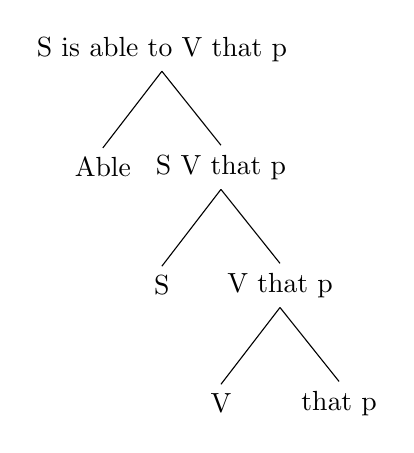
\begin{tikzpicture}[
        ]
        \node{S is able to V that p}
        child {node {Able}}
        child {node {S V that p}
          child {node {S}}
          child {node {V that p}
            child {node {V}
            }
            child {node {that p}
            }
          }
        };
      \end{tikzpicture}
    \end{subfigure}
    %
    \begin{subfigure}{.5\textwidth}
      \centering
      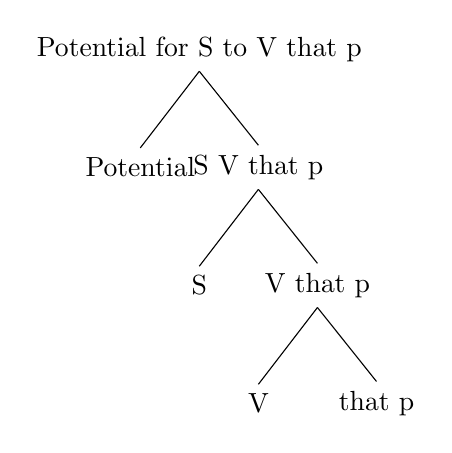
\begin{tikzpicture}[
        ]
        \node{Potential for S to V that p}
        child {node {Potential}}
        child {node {S V that p}
          child {node {S}}
          child {node {V that p}
            child {node {V}
            }
            child {node {that p}
            }
          }
        };
      \end{tikzpicture}
    \end{subfigure}
  \end{figure}
  Suggestion here is that there's really nothing too interesting.
  In both cases it seems possible to have a complete description of the witnessing event prior to the introduction of a modal.
  Only complexity involved is projecting agent from event in order to apply ability.
\end{note}


\begin{note}[Breaking things down]
  An instance of potentive entailment has an antecedent and consequent.
  As may be seen from the examples provided, there are no particular constraints on the consequent of a potentive entailment.
  The antecedent of potentive entailments of interest, however, have two main components:
  \begin{itemize}
  \item\label{pe:part:event} An event.
  \item\label{pe:part:modal} A `potentive' modal applied to the event
  \end{itemize}
  The event in turn has three important components:
  \begin{enumerate}
  \item\label{pe:part:agent} An agent.
  \item\label{pe:part:verb} A verb describing some action performed by the agent.
  \item\label{pe:part:result} Some result of a successful performance of the action described by the verb.
  \end{enumerate}

  Gave a gloss of potentive entailment.

  Key observation 1.
  Possible consequents are determined by the event, rather than the modal.
  Obtain consequent because of the modal.

  So, each of the examples, we obtain the same entailment on the assumption that the event described has happened.

  Contrast.
  Potential for \(e_{1}\) and potential for \(e_{2}\), so potential for \(e_{3}\).
  E.g.\ conjunction introduction.

  In other words, the consequent does not hold because the event is a \emph{potential} event.
  Or, that this is `epistemic'.

  Well, consequent because the event of the antecedent requires the consequent.

  So, that the potential provides a way to get the consequent prior to the event happening.
  No instance of potentive entailment where the consequent follows because the event is potential.
  This is not to deny that there are cases in which entailment relies on potential.

  So, here explaining why the work is done primarily by the verb.
  Might think that using `discovers' is a counterexample.
  Only possible because the action involved is for the moment potential.
  However, the verb itself does the work here.
  Get the consequent that the agent hasn't done the reasoning, but understanding this as simply shifting temporal index.

  So, the important of this key observation is that we further reduce interest in ability.
  We've seen that alternative modal may be used.
  And now that the modal is of secondary importance.

  So, property is seen as surface level.

  Two candidates for the antecedent.
  \begin{quote}
    \begin{enumerate}
    \item There is a potential event in which \emph{S} \emph{V}s that \(\phi\).
    \item \emph{S} has the ability to \emph{V} that \(\phi\).
    \end{enumerate}
  \end{quote}
\end{note}


\subsection{Entailment}
\label{sec:entailment-1}




\begin{note}[Counterfactual]
  One option is counterfactual.
  This is true, and then consider all of those things some that if they we're true, potential wouldn't be true.
  Consider change to the actual world that would result from false consequent, and figure out whether potential still holds.

  Problem here is that counterfactuals are tricky.

  Minimal change may still result in potential.
  Chess example, if strategy doesn't exist, then it's not clear how to understand this.
  Some other rules of chess, and strategy may still exist.
\end{note}

\begin{note}[More direct]
  Preferred option is to consider all witnessing events.
  No matter how things turn out, the truth of \(\phi\) persists throughout event.

  What about changes?
  So, there's some potential event, because of some change to the rules of chess.
  Hence, there is a possible event, but relies on an unexpected development.
  Problem with potential?
  Arguably same issue holds for ability.

  However, it's then going to be the case that there is some change.
  Problem here when it comes to reasons, as the agent doesn't have the reasons available.

  Observation here is that \(\phi\) is an enabling condition.
  Potential just in case that it does not depend on further enabling conditions that are not yet the case.


  So, suggestion that if something holds throughout every event, then it holds of the actual world.
  Basically, this rules out an enabling condition that is not true.

  Hence, \(\phi\) is an enabling condition, and does not require additional enabling conditions.
\end{note}

\begin{note}[Still issue of underspecified event]
  Returning to the matchbox.
  Different preconditions.
  Well, depends on how the event is understood.

  Use this idea to suggest some troubles.
  By, extending events to include establishing what seem to be preconditions.
  Suggest that this is taken care of by understanding of event.
\end{note}

\begin{note}[Some issues with ability]
  Even so, not clear that additional features of ability are desirable.
  For example, conditional analysis.
  S has the ability to \(\phi\), understood as S would \(\phi\) if S tried to.
  (\citeyear[\S4]{Mandelkern:2017aa})
  And act conditional analysis
  \begin{quote}
    there is some practically available action A such that the closest world where S tries to do A is a world where S does \(\phi\)\nolinebreak
    \mbox{}\hfill\mbox{(\citeyear[\S5]{Mandelkern:2017aa})}
  \end{quote}
  Or \cite{Schwarz:2020aa}, who distinguishes two readings.
  \begin{quote}
    \begin{enumerate}[label=\textbf{\alph*.}]
    \item \emph{S} can \(\phi\) (effectively) iff there are (highest-ranked) accessible worlds at which \emph{S} \(\phi\)s.
    \item \emph{S} can \(\phi\) (transparently) iff there are (highest-ranked) accessible worlds at which \emph{S} \(\phi\)s \emph{transparently}.
    \end{enumerate}
    \emph{S} \(\phi\)s \emph{transparently} iff \emph{S} \(\phi\)s as a result of a volitional state that warrants believing that she will \(\phi\) provided that \(\phi\)ing is under her volitional control.
  \end{quote}

  \begin{quote}
    a world is accessible iff it is under the agent’s volitional control --- that is, iff it would result from some available variation of the agent's volitional state.\nolinebreak
    \mbox{}\hfill\mbox{(\citeyear{Schwarz:2020aa})}
  \end{quote}

  Accessible world in which agent has volition.

  
  Counterfactual considerations.
  
  Noted that potential events don't require agents, hence if volitional states of agents, then holds whether volition is precondition for restricted cases.

  Demonstrate someones innocence.
  Well, transparecy.

  Potentive entailment follows even if agent has no volition.
\end{note}

\begin{note}[Transformative experience?]
  \citeauthor{Paul:2014aa}, maybe.
\end{note}

%%% Local Variables:
%%% mode: latex
%%% TeX-master: "masterD"
%%% End:


%%% Local Variables:
%%% TeX-master: "master"
%%% End:

\chapter{Access}
\label{cha:access}

\begin{note}[Basic motivation]
  \ref{denied-claim} provides an account of why an agent has support for some propositions and not others.
  Intuition that in two contrasting cases, one in which the agent does the reasoning, and one in which the agent does not, that the one in which the agent does not is not in a position to claim support.

  As this is only (it seems, relevant) difference, then this motivates~\ref{denied-claim} to some degree.
  However, this kind of motivating is lacking.

  Sam is not tall, Taylor is tall.
  Difference is some fixed height.
  So, tallness requires this particular height.
\end{note}

\begin{note}[Necessary condition]
  \ref{denied-claim} may be strengthened.

  For example, a synchronic/simultaneous requirement.
  \citeauthor{Goldman:2011vn} writes:
  \begin{quote}
    How can evidentialism cope with this problem? It could improve its handling of these cases by abandoning the simultaneity requirement, the requirement that justifying evidence must be possessed at the same time as the belief. But this requirement is a core part of internalism, to which mentalist evidentialism adheres.\nolinebreak
    \mbox{}\hfill\mbox{(\citeyear[261]{Goldman:2011vn})}
  \end{quote}
\end{note}

\begin{note}[Requires foundationalism?]
  Might want to deny~\ref{denied-claim} as it seems to weakly conflict with coherentism, for example.

  For,~\ref{denied-claim} suggests a basing relation, and this doesn't seem to work too well with coherentism.
  Either coherentism is false, or coherence doesn't make a difference in cases of reasoning.
  Neither seem plausible.

  Suggest that there is a plausible revision.

  In the literature, there's attempts to make this work.
  Especially with regard to credences.

  \textcite[\S2]{Silva:2020aa} has some pointers.
\end{note}

\section{Generalising uRA to all instances of reasoning}
\label{sec:generalising-ura-all}

\begin{note}[Broader conditional]
  Still, the observations made when establishing~\ref{P:ab-and-dc:W} broader relation between \ref{denied-claim} and ability.
  For, we noted that \ref{denied-claim} is incompatible with \WR{}.
  To recap:
  \begin{enumerate}[label=(B\arabic*), ref=(B\arabic*)]
  \item Assume an agent appeals to entailment from the ability to \emph{V} that \(\phi\) in order to obtain \(\phi\).
  \item The agent makes use of (the reasoning sketched in) either \AR{} or \WR{}.
  \item \WR{} is incompatible with~\ref{denied-claim}.
  \item The agent makes use of (the reasoning sketched in) \AR{}.
  \end{enumerate}
\end{note}



\section{Literature}
\label{sec:literature}

\subsection{Simple instances}
\label{sec:simple-instances}

\begin{quote}
  A person may know some propositions that logically entail some proposition that the person scarcely understands and surely does not know to follow from the things she does know.
  The logical route from what she knows to this proposition may be complex and go beyond her understanding, or even the understanding of any person.
  In our view, the person is not then justified in believing the consequence, even though it is entailed by her evidence.
  It is noteworthy that, to become justified in believing the proposition, she has to learn something new---namely, its logical connection to her evidence.\nolinebreak
  \mbox{}\hfill\mbox{(\citeyear[94]{Conee:wk})}
\end{quote}
Falls a little short.
Talking about a specific kind of proposition.
Interest is in the suggestion for why this fails.
Still, doesn't require the agent to reason.
However, this is a natural variant of~\ref{denied-claim}, {\color{red} and I should make this clear when introducing the claim that this variant is available}.


\subsection{\citeauthor{Littlejohn:2018uq} and forking paths}
\label{sec:littlejohn}

\textcite{Littlejohn:2018uq} denies the path principle:

\begin{quote}
  The Path Principle: The types of support relations that hold between a thinker's evidence and the propositions she grasps wholly determine whether there is propositional justification for believing these propositions.\nolinebreak
  \mbox{}\hfill\mbox{(\citeyear[224]{Littlejohn:2018uq})}
\end{quote}

Failure of the path principle is similar to failure of~\ref{denied-claim}.
In that, there are cases in which agent has something without accessing support.
proposition support, but so long as it is possible for the agent to obtain doxastic support, then this is something similar.
Different, however, in the details.
\ref{denied-claim} concerns cases of reasoning from premises to conclusion.
So, compatible with failure of the path principle in cases which do not involve reasoning.

\citeauthor{Littlejohn:2018uq} observes the following two corollaries of the path principle.

\begin{quote}
  The Dependence Thesis: There is no situation in which it is appropriate for a thinker to believe p where the thinker does not possess evidence that provides the right support for believing p.\nolinebreak
  \mbox{}\hfill\mbox{(\citeyear[227]{Littlejohn:2018uq})}
\end{quote}

\begin{quote}
  The Sufficiency Thesis: There is no situation in which a thinker's evidence provides the right support for believing p if there is a situation where this type of evidential support relation fails to provide sufficient support for believing a suitable counterpart of p.\nolinebreak
  \mbox{}\hfill\mbox{(\citeyear[227]{Littlejohn:2018uq})}
\end{quote}

\citeauthor{Littlejohn:2018uq} argues against these:

\begin{quote}
  The first problem has to do with the Dependence Thesis.
  However we understand evidence and its possession, there are some cases of justification without evidential support.
  The second problem has to do with the Sufficiency Thesis.
  Even when there is evidence that supports a proposition that a thinker justifiably believes, that type of support might hold in other cases and fail to justify a thinker's beliefs.\nolinebreak
  \mbox{}\hfill\mbox{(\citeyear[227]{Littlejohn:2018uq})}
\end{quote}

It is only \citeauthor{Littlejohn:2018uq}'s argument against the sufficiency thesis that relates to~\ref{denied-claim}.
However, this trades on whether what the agent has is always sufficient.
Hence, requires cases in which the agent has support.




\section{Basing and \ref{denied-claim}}

\begin{note}[Basing]
  Following \citeauthor{Silva:2020aa}:
  \begin{quote}
    \textbf{(Basing)} S's belief that p is appropriately connected to S's sufficient epistemic reasons, R, to believe that p iff S's belief that p is based on R.\linebreak
    \mbox{}\hfill\mbox{(\citeyear{Silva:2020aa})}
  \end{quote}
\end{note}


\begin{note}[No doxastic support]
  A little more work to argue that the agent does not have doxastic support.
  Idea is to assume that agent forms attitude, and question whether it satisfies basing requirement.
  In part,~\ref{denied-claim}.
\end{note}

\begin{note}[Examining doxastic via basing]
  Following paragraphs serve two purposes.
  First, variety of accounts of basing are incompatible with doxastic support.
  Second, that the support in doxastic support is no different from support in propositional support --- relation to the agent.

  If already convinced, then may skip ahead.
\end{note}

\begin{note}[Taxonomy of basing]
  Follow taxonomy presented by \textcite{Korcz:2021ue}.
  \begin{itemize}
  \item Causal.
  \item Counterfactual.
  \item Doxastic.
  \item Causal-doxastic.
  \end{itemize}
\end{note}

\begin{note}[Causal]
  Causal is ruled out, as we're interested in support from general ability, roughly, and there's no plausible causal relation.
  The information that specific ability follows does the work.

  \cite{Moser:1989tv}
  \begin{quote}
    \emph{S}'s believing or assenting to \emph{P} is based on his justifying propositional reason \emph{Q} \(=_{\text{df}}\) \emph{S}'s believing or assenting to \emph{P} is causally sustained in a nondeviant manner by his believing or assenting to \emph{Q}, and by his associating \emph{P} and \emph{Q}.\nolinebreak
    \mbox{}\hfill\mbox{(\citeyear[157]{Moser:1989tv})}
  \end{quote}

  \begin{quote}
    \emph{S} occurrently satisfies an association relation between \emph{E} and \emph{P} \(=_{\text{df}}\)
    \begin{enumerate*}[label=(\roman*)]
    \item \emph{S} has a \emph{de re} awareness of \emph{E}'s supporting \emph{P}, and
    \item as a nondeviant result of this awareness, \emph{S} is in a dispositional state whereby if he were to focus his attention only on his evidence for \emph{P} (while all else remained the same), he would focus his attention on \emph{E}.
      \newline
      \mbox{}\hfill\mbox{(\citeyear[141--142]{Moser:1989tv})}
    \end{enumerate*}
  \end{quote}

  \cite{Ye:2019ux}
  \begin{quote}
    \textbf{Causation Caused by Believing (CCB)}

    One's belief that p is based on reason R just in case R causes the belief and the causation is caused by one's believing that R supports p.
    \newline
    \mbox{}\hfill\mbox{(\citeyear[27]{Ye:2019ux})}
  \end{quote}
  In our cases, no causation from premises.
  Further, if agent considers \nI{}, then won't get the second part of supporting relation.
\end{note}

\begin{note}[Counterfactual]
  Counterfactual.
  Based on reason is caused or would have caused in appropriate circumstances.
  So, belief ends up being based on all pseudo-overdeterminants, for example.
  Built in to \citeauthor{Swain:1981wd}'s account is that the agent did some reasoning, and over-determinant is a substitute for reasoning performed.

  Here, may suggest that agent has done some reasoning, as they've gone from ability to conclusion.
  This reduces to an instance of \AR{} in order for agent to obtain support on reasoning \emph{performed}.
  No clear modification, as then agent would end up with a basic relation in cases where no relation obtains.
\end{note}

\begin{note}[Doxastic]
  Doxastic.
  \cite{Tolliver:1982us}

  \begin{quote}
    \begin{enumerate}[label=(B)]
    \item A bases his belief that q on p at time t, iff
      \begin{enumerate}[label=(\arabic*)]
      \item A believes that q at t and A believes that p at t, and
      \item A believes that the truth of p is evidence for the truth of q at t, and
      \item \space[\dots]\footnotemark
        \mbox{}\hfill\mbox{(\citeyear[159]{Tolliver:1982us})}
      \end{enumerate}
    \end{enumerate}
    \footnotetext{
        The final condition is designed to rule out certain problematic cases which expands on \citeauthor{Tolliver:1982us}'s understanding of what it is for the truth of p to be evidence for the truth of q.
        \begin{quote}
        \begin{enumerate}[label=(\arabic*)]
          \setcounter{enumi}{2}
        \item Where A's estimate of the likelihood of q equals h at t \(0 < h \leq 1\), \emph{if it were the case that}:
          \begin{enumerate}[label=(\roman*)]
          \item A's second·order estimate ofthe L-proposition ``the likelihood of q is greater than or equal to h'' is less prior to t than it at t, and
          \item A did not believe p prior to t, and
          \item A came to belive pa at t,
          \end{enumerate}
          then, at t, A's second-order estimate of the L-proposition ``the likelihood of q is greater than or equal to h'' would be greater than it was prior to t.
          \end{enumerate}
        \end{quote}
      }
    \end{quote}
    The second condition qualifies \citeauthor{Tolliver:1982us}'s account as doxastic.
    The agent has a `meta-belief' that that the truth of the reason is evidence for the truth of the content of the agent's belief.
    For example, agent believes that the premises available for existence of (particular) strategy are evidence for existence of strategy.
    This does not require a causal relation between the reason and the belief, or between the relevant premises and the existence of the (particular) strategy.

    Feature of the meta-belief is that it is not part of the established basing relation.

    Two issues with \citeauthor{Tolliver:1982us}.
    A component of the first condition --- believing p at t --- and the second condition.

    On certain accounts of belief, believing p at t, will hold true.
    Whatever the relevant premises are, the agent believes them.
    However, this is not particularly clear.

    The second condition is the primary difficulty.
    Motivated by \citeauthor{Lehrer:1971aa}.
    \cite{Korcz:2000uo} outlines the argument (\citeyear[534]{Korcz:2000uo}).
    Hence, suggests such meta-beliefs are sometimes sufficient to establish basing relation.

    \citeauthor{Tolliver:1982us} talks of belief, \citeauthor{Korcz:2000uo} talks interchangeably of awareness or meta-belief.
    Continue to talk of meta-belief.

    \citeauthor{Tolliver:1982us} provides an analysis of what it is to believe that the truth of p is evidence for the truth of q. (\citeyear[156--157]{Tolliver:1982us})
    Key is that \citeauthor{Tolliver:1982us}'s condition requires the agent to have information about the relation.
    Incompatible with cases of interest, where agent doesn't have information about how (specific) ability leads to conclusion.

    \citeauthor{Korcz:2000uo} proposes that p and q contribute to causing the meta-belief.
    So, this suggests that the only cases are those in which there's some rewriting of an established basing relation.

    If follow \citeauthor{Korcz:2000uo}, then it seems as though we exclude instances of `first time' support.
    If we continue to follow \citeauthor{Tolliver:1982us}, then support for meta-belief.

    If don't require support, then things get difficult.
    On the one hand, problematic examples \citeauthor{Korcz:2000uo} mentions.
    As noted, \citeauthor{Korcz:2000uo} uses causation.
    Could substitute with some kind of support, but this kind of support is absent from scenarios of interest.

    On the other hand, if restricted independently of support, then it seems many basing instances are going to come for free.


  Here we have a kind of meta-belief about relation of support.
  As with counterfactual, the issue is with the meta-belief.
  No clear way to establish this without a variant of \AR{}.
  Here, this doesn't require~\ref{denied-claim}, which may be of some interest.

  Causal-doxastic inherit the problems of more basic.

  Upshot is that following the taxonomy, there's no clear basing relation in scenarios of interest.
  Influence of~\ref{denied-claim}.

  Of course, doesn't establish, as not requirement that doxastic support requires one such account of basing relation.
  However, more than suggestive that there's no doxastic support.

  
\end{note}

\begin{note}[Example of \citeauthor{Neta:2019aa} on basing]
    \begin{quote}
    For an agent A to C for reason R involves A’s \emph{de se}, object-involving representation of a particular explanatory relation between R, on the one hand, and her C’ing, on the other, and that object-involving representation represents that same explanatory relation under the category ex post justifying.\nolinebreak
    \mbox{}\hfill\mbox{(\citeyear[204]{Neta:2019aa})}
  \end{quote}
  Distinct from other accounts.

  \emph{De se} so that there no possible mistake about whether it is the agent that is C'ing.
  The explanatory connexion is represented.
  \citeauthor{Neta:2019aa} is non-committal to what is involved with representation.

  Key is `\emph{that same explanatory relation}'.
\end{note}

\begin{note}[Summarising]
  Seems plausible to grant that the agent has propositional support.
  Similarly plausible that the agent does not have doxastic support.

  Doxastic support captures something stronger than what is available to the agent.
  By doing reasoning, agent would establish doxastic support.

  Still, do not need to claim doxastic support.
  Goal is to allow agent to establish support from premises.
  This may fall (qualitatively) short of being doxastic support.

  Interest with above, as this is intuitively a case of, or closely related to, basing.
\end{note}


\section{Notes}
\label{sec:notes}

\begin{note}[Memory]
  \ref{denied-claim} doesn't require that the agent continues to have access to reasons.

  \textcite[208]{Goldman:1999tr} has a nice statement regarding the \emph{problem of forgotten evidence} for internalism.
  \ref{denied-claim} only concerns the agent obtaining something like `first-time' support.
  If agent reasons to conclusion from premises, and forgets premises, remains true that the agent obtained support by reasoning from those premises.
\end{note}

%%% Local Variables:
%%% TeX-master: "master"
%%% End:


\chapter{Inertia}
\label{cha:inertia}

\section{Inertia}
\label{sec:inertia}

Argument against~\ref{denied-claim} is that it conflicts with \nI{-} in scenarios highlighted by~\ref{prem:ab}.

\begin{enumerate}[label=\nI{}, ref=\nI{}]
\item An agent is not able to obtain support for some proposition \(\psi\) on the basis of information that some the support the agent has for \(\phi\) is misleading or mistaken if \(\psi\) is not the case.
\end{enumerate}

There is lack of an explanatory connexion between support for \(\phi\) and support for \(\psi\).

\section{nI}
\label{sec:ni}

Case in which the support the agent has does not trace from access, or the agent obtains support on the basis that the support the agent does have is misleading.

Note, talk about `obtaining' support.
So, we have a setup where:

\begin{enumerate}
\item Agent has support.
\item Say, for some proposition \(\psi\).
\item The support for \(\psi\) is not, given the agent's doxastic state, also support for \(\psi\).
\item Agent receives information to the extent that the agent's support for \(\psi\) is misleading if \(\psi\) is not the case.
\item Agent holds that the support for \(\psi\) supports \(\phi\) being the case, because else their support is misleading.
\end{enumerate}

Here, the support doesn't do anything for \(\phi\).

This principle is less obvious, but I think fine.

Consider a few good cases and some bad cases.

Good case, deduction.
So, if support for \(\phi\) then support for \(\phi \lor \psi\), because, intuitively, support for \(\phi\) is also support for \(\phi \lor \psi\).
It is puzzling to motivate on the basis that the agent obtains support for \(\phi \lor \psi\) because if \(\phi \lor \psi\) is not the case then their support for \(\phi\) would be misleading.
Of course, this is the case.
However, that is not why the agent has support for \(\phi \lor \psi\).


Suppose quiz.
Interested in answer to a certain question, mix with questions I know the answer to.
Contestant gets the answers correct.
Support that the contestant is good with respect to the domain.
Have support for the question I'm interested in.

Problem if that I hold the answer to the question is such and such because otherwise support for contestant understanding the domain would be misleading.

These are two cases where things look straightforward, and the agent has support by some other route.

If X then support is misleading
Therefore, not-X.

???

If that's not a boat then the radar is faulty.

Have support that the radar is working well.
So, it is a boat.

??? Though in this case it looks as though there's a way to go from functioning radar to boat.

Slight variant.
Checked the radar, support that it's functioning correctly.
Not looking at the screen.

If there's a blip on the radar, then it's not functioning correctly.
Support that it's functioning correct.
So, there's no blip on the radar.



Parked car outside.
If car is stolen then support that this is a safe neighbourhood would be misleading.
Support for car is not stolen.


If the seeds haven't started sprouting yet, then you've been misled about the planting conditions.
Have not been misled about the planting conditions.
So, the seeds have started sprouting.

\begin{note}[Denying~\nI{}]
  Worry about coherence.

  If the agent does not obtain support, then in a situation where:
  \begin{itemize}
  \item Support for \(\phi\)
  \item Information that if \(\phi\) is the case then \(\psi\) is the case.
  \item No support for \(\psi\).
  \end{itemize}

  So, agent is committed in some sense to \(\psi\) being the case, given the support they have for \(\phi\) and the information.

  I have support for \(\phi\) and information that \(\phi \rightarrow \psi\), but no support for \(\psi\).

  Looks like a failure of closure.

  However, closure is typically formulated with entailment.
  In each of these cases, there's no entailment.
  Distinction between the support for \(\phi\) and \(\phi\).

  Would need something to the effect of positive attitude only if support.

  However,~\nI{} only denies support.
  It does not deny that the agent is require to have some positive attitude toward the proposition.
\end{note}

\begin{note}[Undercutting defeaters]
   Undercutting defeaters are of interest with respect to~\nI{} is that (merely) suggesting that the agent's support for \(\phi\) is no good can amount to highlighting that the agent's support for \(\phi\) may be misleading.

  Consider the following illustration provided by \citeauthor{Pollock:1987un}\nolinebreak
  \footnote{
    \citeauthor{Pollock:1987un} defines an undercutting defeater as follows:
    \begin{quote}
      R is an \emph{undercutting defeater} for P as a prima facie reason for S to believe Q if and only if
      \begin{enumerate}[label=(UD\arabic*), ref=(UD\arabic*)]
      \item P is a reason for S to believe Q and R is logically consistent with P but (P and R) is not a reason for S to believe Q, and
      \item R is a reason for denying that P wouldn't be true unless Q were true.\nolinebreak
        \mbox{}\hfill\mbox{(\citeyear[485]{Pollock:1987un})}
      \end{enumerate}
    \end{quote}
    Intuitively, an undercutting defeater for P as a reason for Q because it the defeater denies that Q must be true in order for P to be true.
  }\nolinebreak
  :
  \begin{quote}
    [Undercutting defeaters] attack the connection between the reason and the conclusion rather than attacking the conclusion itself.
    For instance, ``X looks red to me'' is a prima facie reason for me to believe that X is red.
    Suppose I discover that X is illuminated by red lights and illumination by red lights often makes things look red when they are not.
    This is a defeater, but it is not a reason for denying that X is red (red things look red in red light too).
    Instead, this is a reason for denying that X wouldn't look red to me unless it were red.\nolinebreak
    \mbox{}\hfill\mbox{(\citeyear[485]{Pollock:1987un})}
  \end{quote}
  Completing \citeauthor{Pollock:1987un}'s example, it seems that if agent's support for holding that X is red is that `X wouldn't look red to me unless it were red', then the support for X being red provided by appearance is retracted after discovering that X is illuminated by red lights (though it remains possible that X is red).

  Assumption --- in violation of \nI{} --- an agent always has the option to obtain support for \(\psi\) on the basis of information that the support the agent has for \(\phi\) is misleading if \(\psi\) is not the case.

  Given that it remains possible that X is red, it follows that the appearance of X being red would be misleading if X is not red.
  For, it continues to be the case that X appears to be red, even after the discovery is made by the agent.
  Therefore, by the assumption violating~\nI{}, support for X being red persists in the presence of the undercutting defeater.
  Still, intuitively it seems that the undercutting defeater of a red light blocks the agent obtaining support for X being red on the basis of their visual perception.

  This is partial motivation for~\nI{}, as substituted `does not have the option' from the text of~\nI{} with `always has the option' when making the problematic assumption.
  Further argument is (hopefully) to follow.

\end{note}


\section{Motivation for \nI{}}
\label{sec:motivation-ni}

\begin{itemize}
\item Because, the support the agent has is independent of \(A(\psi)\)/\(\psi\).
\end{itemize}

\begin{itemize}
\item An agent is not able to obtain support for some proposition \(\psi\) on the basis of information that the support the agent has for \(\phi\) is misleading if \(\psi\) is not the case.
\end{itemize}

\begin{itemize}
\item The relevant information must also provide some support for \(\phi\).
\item One way of getting to this is by ordering support.
\item If the constraint is established prior to obtaining support, then this may limit support.
\end{itemize}

\begin{itemize}
\item This is also related to Harman.
\item For, the principle there is that one is not in a position to hold that support is going to be misleading.
\item Support for \(\phi\) does not show that future support for \(\psi\) is misleading when \(\psi \vdash \lnot\phi\).
\item Support for \(\phi\) does not show that\dots
\end{itemize}

\begin{itemize}
\item Important to note is that this does not deny closure.
\item First, doxastic.
\item Second, no requirement that the required information is a (known, logical) entailment.
\end{itemize}

Why does witnessing work?

\begin{itemize}
\item Because the agent is not basing things on the support they have.
\item The things about misleading support is that it doesn't say there's anything problematic about the information received.
\end{itemize}

\subsection{Motivation, taken from overview}
\label{sec:motiv-taken-from}

\begin{note}[Some motivation for \nI{}, 1]
  Some motivation for~\nI{} may be found by constructing instances of reasoning which violate~\nI{}.
  A couple of cases may help.

  For example, suppose our agent is out shopping for a gift for Sam with a friend and has not yet considered the items before them.
  The friend remarks that `Someone would only buy \emph{that} (some particular item) as a gift for Sam if they didn't know Sam very well.'
  The agent has support that they do know Sam very well.
  However, it does not seem permissible for the agent to obtains support that they wouldn't buy that as a gift, one the basis of the support they have their familiarity with Sam and the statement made by their friend.
  For, it is possible that they agent would have settled on the particular item if they had given it some consideration --- the support the agent has for their familiarity with Sam \emph{may} be misleading.

  Or, suppose the agent has parked their car on the street outside of Sam's place and reasons that:
  If my car is stolen then my support that this is a safe neighbourhood would be misleading.
  Therefore, as my support that this is a safe neighbourhood is not misleading, my car has not been stolen.
  The agent's reasoning seems confused.
  Perhaps the agent has the option of extending the support the have that the neighbourhood is safe to obtain support that they car remains parked outside, but that support the agent has would be misleading if their car has been stolen does not seem appropriate.
\end{note}

\begin{note}[Some motivation for \nI{}, 2]
  For further motivation, consider undercutting defeaters.

  We take the following sketch from \textcite{Worsnip:2018aa}:
  \begin{quote}
    Undercutting defeaters, which are easiest to think of in the context of the attitude of belief, are supposed to be considerations that undermine the justification of a belief in a proposition p not necessarily by providing (sufficient) positive evidence to think that p is false, but rather merely by suggesting (perhaps misleadingly) that one’s reasons for believing p are no good, in a way that neutralizes or mitigates their justificatory or evidential force.\nolinebreak
    \mbox{}\hfill\mbox{(\citeyear[29]{Worsnip:2018aa})}
  \end{quote}
\end{note}


\subsection{Misleading support}
\label{sec:misleading-support}

\begin{note}[Misleading, again]
  By the support that the agent has for some proposition being \emph{misleading} we mean that the support the agent has for \(\phi\) provides good reason for thinking that \(\phi\) is the case, even if \(\phi\) is not the case.\nolinebreak
  \footnote{
    Different from `mistaken', where \(\phi\) turns out to be true, but the support itself provides the wrong understanding of why \(\phi\) is true.

    Suspect that a variant of \nI{} holds for `mistaken'.
    However, `misleading' is sufficient.
  }
  For example, see someone entering a car by unlocking the drivers door with a coat-hanger.
  I take this to be good support for the proposition that the person is not the owner of the car.
  As it turns out, the person had accidentally locked their only set of keys in the car, and did not want to call a locksmith.
  The support for the proposition that the person is not the owner of the car was misleading, not only because the person owns the car, but because it continues to provide support even with the knowledge that the person is the owner.
  It would be clear to the owner why they would be stopped by a police officer, and why the owner is required to provide documentation to show that they are the owner (i.e.\ support to the contrary proposition).

  In this sense, the support is misleading.
  The support is `good', even though the proposition is false.

  `Misleading' support is distinct from an error made by the agent, such as taking the use of the coat-hanger to be support for the proposition that the someone had stolen the person's coat and locked the coat inside the car.\nolinebreak
  \footnote{
    No doubt there is additional background that could be added\dots
  }
  And, misleading support is distinct from `mistaken' in which an agent obtain support for some proposition which is true but where some part of the support is false.

  For example, person using the coat-hanger looks like the owner, but the car had recently been sold.
  In contrast to error, there seems no problem with the agent holding a positive attitude toward the proposition given mistaken and misleading support, the relevant difference is whether the proposition does hold.

  Intuitively, then, the trouble with misleading support is that it suggests, but does not ensure that the proposition holds.

  Misleading support, then, is not problematic.
\end{note}


\begin{note}[Combination]
  \nI{} and \nIm{} combine:

  \begin{proposition}[\nIp{}]
    An agent does not have the option of claiming support for some proposition \(\xi\) from observing that \(\psi\) entails \(\xi\) and information that the support the agent claims for \(\phi\) is misleading if \(\psi\) is not the case.
  \end{proposition}

  With respect to scenarios of interest.
    \(\phi = \) general ability.
    \(\psi = \) specific ability.
    \(\xi = \) strategy exists.

    So, application of \nI{} (and \nIm{}) is that the agent does not have option of obtaining support for specific ability from information that the support they have for general ability is misleading if the agent does not have the specific ability.

    Stated independently, \nIp{} is a weaker proposition than \nI{} and \nIm{}.\nolinebreak
    \footnote{
      as \nIp{} makes no statement about whether the agent may claim support for \(\psi\) (though \nI{} does).

      From \nI{}, the agent does not get support for \(\psi\), and by \nIm{} agent requires support for \(\psi\) to get support for \(\xi\), and hence does not obtain support for \(\xi\).

    Still, as it is the result of interest, some room to pursue the present line of argument if either \nI{} or \nIm{} is rejected.
    }
    Suspect that any argument from \nIp{} follows from motivation for \nI{} and \nIm{}.

  If \nI{} (and \nIm{}) hold, then trouble if support for specific ability comes from general being misleading if general is not the case.
\end{note}


\begin{note}[Relation to transmission]
  Here, difference to failure of transmission.
  In those cases, agent knows, hence \(\phi\) not being true is not much of an issue.
  In turn, \(\psi\).

  For us, \(\phi\) may be false.

  Whether there is a proper distinction, though, isn't quite so easy.
  Dogmatism gets thrown into the mix.
\end{note}


\begin{note}[Things not claimed]
  Don't appeal to possibility that support for \(\psi\) will be stronger for \(\psi\) having different value.
  Support isn't sufficiently strong.\nolinebreak
  \footnote{
    This requirement distinguishes from transmission failure.
  }
  Given that \(\psi\) is a dependency, \(\psi\) may be why strength of support is limited.
  And, from the above, lack of use of support for \(\psi\), hence agent is not in a position to go either way.
\end{note}


\section{Relatated literature}
\label{sec:relatated-literature}

\begin{note}[Related to\dots]
  Focus is on support.
  A pair of related things to illustrate interesting parts of \nI{}.
\end{note}

\begin{note}[No feedback/Bootstrapping]
  No feedback by \citeauthor{Weisberg:2010to}.

  \begin{quote}
    \textbf{No Feedback} If
    \begin{enumerate*}[label=(\roman*), ref=(\roman*)]
    \item\label{WB:NF:1} \(L_{1}-L_{n}\) are inferred from \(P_{1}-P_{m}\), and
    \item\label{WB:NF:2} \(C\) is inferred from \(L_{1}-L_{n}\) (and possibly some of \(P_{1}-P_{m}\) by an argument whose justificatory power depends on making \(C\) at least \(x\) probable, and
    \item\label{WB:NF:3} \(P_{1}-P_{m}\) do not make \(C\) at least \(x\) probable without the help of \(L_{1}-L_{n}\), then the argument for \(C\) is defeated.\nolinebreak
      \mbox{}\hfill\mbox{(\citeyear[533--534]{Weisberg:2010to})}
    \end{enumerate*}
  \end{quote}

  Some similarities.
  Stated in probabilistic terms, so no easy application.
  And, addition of \(C\) condition.
  Expand to add this.

  Somewhat different.
  For, inclusion of support, which (at least without further work) is qualitative rather than quantitative.
  So, it seems \ref{WB:NF:3} isn't going to hold.

  Still, reform No Feedback a little.
  Consider \ref{WB:NF:3} from the agent's point of view, independent of whether \(P_{1}-P_{m}\) not make \(C\) at least \(x\) probable.
  Plausibly problematic if agent doesn't have response to~\ref{WB:NF:3}.
  And, this would be issue of not showing how \(P_{1}-P_{m}\) relate to \(L_{1}-L_{n}\).
\end{note}

\begin{note}[Bootstrapping and reliabilism]
  \nI{} is distinct from No Feedback, but shares some similarities.
  Attempted to keep to weak principles regarding support --- primarily \eiS{}.
  Given relation to No Feedback, may question, as No Feedback applies to bootstrapping, following from reliabislim.
  Hence, worry, as something sufficient to deny reliabilism is somewhat strong.

  Quick argument is that \nI{} is silent with respect to (at least some) instances of reasoning ruled out by anti-bootstrapping principles.
  Hence, \nI{} will not entail bootstrapping, and seems compatible with reliabilism.

  Focus on knowledge.
  However, justification also.
  Here, work with example from \textcite{Cohen:2010ux}, as this is designed for justification.\nolinebreak
  \footnote{
    Though, structurally similar to instance from \cite{Vogel:2000tl}.
  }

  \begin{quote}
    Suppose, having no idea whether my color vision is reliable, I decide to test it. I have someone stand across the room from me and hold up colored cards one at a time. I look at the first card and reason:
    \begin{enumerate}[label=(\arabic*)]
      \setcounter{enumi}{3}
    \item Card 1 looks red.
    \item Card 1 is red.
    \item Card 1 looks red and is red.
    \item So my color vision worked correctly.
    \end{enumerate}
    \[\vdots\]
    I reason the same way for each of the other cards: card 2 looks green, car 2 is green, so so card 2 looks green and is green, etc. I then infer

    \begin{enumerate}[label=(\arabic*), resume]
    \item My color vision worked correctly every time, i.e., I made no errors.
    \end{enumerate}

    Then I infer inductively that

    \begin{enumerate}[label=(\arabic*), resume]
    \item My color vision is reliable.\nolinebreak
      \mbox{}\hfill\mbox{(\citeyear[142]{Cohen:2010ux})}
    \end{enumerate}
  \end{quote}

  Two questions.
  Whether final step is \RBV{} and if so, whether support is included.

  Final step is induction.
  Plausible that it is.
  Issue, then, is whether inclusion.
  Induction is required, but unclear if not induction, so unclear that there's a plausible account of inclusion.

  If not by value, then the agent isn't required to go by value, and hence \nI{} doesn't apply.

  So, it seems \nI{} does not entail other bootstrapping principles.
  Of course, principles may hold.
  Still, \nI{} is sufficient rather than necessary.

  Simple upshot is that assumed principles about support seem quite weak.
\end{note}

\begin{note}[Wright on transmission failure]
  {
    \color{red}
    Given details on bootstrapping, may be best to leave \citeauthor{Wright:2011wn} to a later chapter.
  }
  The key idea behind \citeauthor{Wright:2011wn}'s account of transmission failure is whether something is a presupposition of a cognitive project.
  Failure when agent uses result of cognitive project to claim warrant for something that was presupposed.
  Hence, a kind of circularity.

  \nI{} is different.
  Does not require \(\psi\) to be a presupposition.
  Agent does not need to presuppose novel application of basis of support for some proposition in order to claim support for some other proposition --- or to be diligent, it is not clear to me that this is the case.

  To illustrate, different readings on Moore's proof.
  For \citeauthor{Wright:2011wn}, presupposition of cognitive project that sight is factive.
  So, this already gets that there's an external world.

  For \nI{}, problem if one thinks that appearance of hand also applies to existence of external world.

  Here, if follow \citeauthor{Wright:2011wn}, then support won't also extend, as presupposed.
  Alternatively, one may argue that the support is for world and hands.
  Hence, that support for world comes from a reapplication of the support used for hands.

  So, this distinguishes \nI{} from transmission failure.
  More is said in chapter~\ref{cha:inertia}.
\end{note}

\begin{note}[Wright: Key difference]
  The key difference with respect to \citeauthor{Wright:2016wl} is that for \citeauthor{Wright:2016wl} the relevant propositions are presuppositions of a cognitive project \emph{and} that the agent is not in a position to claim support for the presuppositions of the cognitive project they are participating in.
  For us, we do not hold that the relevant instance of \(\psi\) needs to be a presupposition of the cognitive project, \emph{nor} that the agent is not in a position to claim support for \(\psi\).

  {
    \color{red}
    This should be reworded.
    The key observation is that \(\psi\) needs to either be, or be entailed by, a presupposition of the cognitive project.
    Therefore, as we don't require this, things are different.
  }
\end{note}

\section{Two Different Ways of Claiming Support}
\label{sec:two-different-ways}

\begin{note}
  Here, two different ways of claiming support.
  \RBV{-} is used when stating \nI{}, so it may be helpful to clarify.
  \incl{} is not used anywhere, but it provides a useful contrast to \RBV{}.
\end{note}

\subsection{Inclusion}
\label{sec:inclusion-support}

\begin{note}[Inclusion of support]
  \begin{proposition}[Inclusion of support --- \incl{}]
    Support for \(\phi\) includes/requires support for \(\psi\).
    If, possible to reapply premises that establish \(\phi\) to establish \(\psi\) (without appealing to value of \(\phi\)).
  \end{proposition}
  Basic idea of \incl{} is reapplication.
  Hence, \incl{}\dots

  Without going by \(\phi\).
  This is not an additional condition, but clarification.
  For, given \eiS{}, agent did not need value of \(\phi\) in order to claim support for \(\phi\), and as agent is reapplying claimed support for \(\phi\), such reapplication does not require value of \(\phi\) either.

    \begin{figure}[H]
    \begin{subfigure}{.45\textwidth}
      \centering
      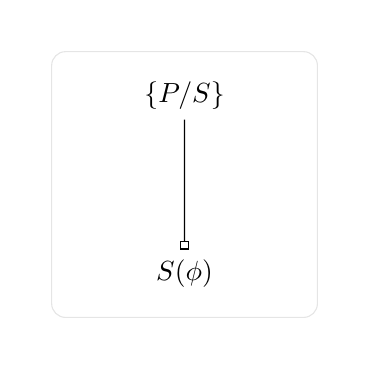
\begin{tikzpicture}[->, >=stealth', node distance=0cm, every text node part/.style={align=center}, scale=0.75]
        \node [] (1) at (-1,4) {};
        \node [] (2) at (-1,-1) {};
        \node [] (3) at (4,-1) {};
        \node [] (4) at (4,4) {};

        \node [] (a) at (1.5,3) {\(\{P/S\}\)};
        \node [] (b) at (1.5,0) {\(S(\phi)\)};
        \node [] (c) at (3,0) {};
        \node [] (d) at (3,3) {};

        \draw [->,-{Square[open]}, xshift=4] (a) to  node[right] {} (b);
        \draw [rounded corners=5pt, opacity=.1] (-.75,3.75) -- (-.75,-.75) -- (3.75,-.75) -- (3.75,3.75) -- cycle;
      \end{tikzpicture}
      \caption{Support for \(S(\phi)\) from premises/steps}
    \end{subfigure}
    \hfill
    \begin{subfigure}{.45\textwidth}
      \centering
      \begin{tikzpicture}[->, >=stealth', node distance=0cm, every text node part/.style={align=center}, scale=0.75]
        \node [] (1) at (-1,4) {};
        \node [] (2) at (-1,-1) {};
        \node [] (3) at (4,-1) {};
        \node [] (4) at (4,4) {};

        \node [opacity=.33] (a) at (.25,3) {\(\{P/S\}\)};
        \node [opacity=.33] (b) at (.25,0) {\(S(\phi)\)};
        \node [] (lt) at (1.5,3.25) {\(\leadsto\)};
        \node [] (dv) at (1.5,3) {\hdashrule[0.5ex][c]{12pt}{.1pt}{}};
        \node [] (ss) at (1.5,2.75) {\(\supseteq\)};
        \node [] (c) at (2.75,0) {\(S(\psi)\)};
        \node [] (d) at (2.75,3) {\(\{P'/S'\}\)};

        \draw [->,-{Square[open]}, opacity=.33] (a) to  node[right] {} (b);
        \draw [->,-{Square[open]},] (d) to  node[right] {} (c);
        \draw [rounded corners=5pt, opacity=.1] (-.75,3.75) -- (-.75,-.75) -- (3.75,-.75) -- (3.75,3.75) -- cycle;
      \end{tikzpicture}
      \caption{Reapply premises/steps to claim support for \(\psi\)}
    \end{subfigure}
    \caption{\incl{} diagram}
  \end{figure}

  Examples:
  \begin{itemize}
  \item \(p \rightarrow r\), includes support for \(p \rightarrow (q \land r)\) with premises \(p \rightarrow q\) and \(q \rightarrow r\).
  \item More complex example of entailment.
  \item Combining support for novel entailments.
  \item If understand language, then parse: some sentence.
  \item Optimal route to some place, then stop at some intermediate point at some time.
  \item Calculation of area, then calculation of diagonal. (A little trickier, as diagonal is background, and it's only the reuse of measurements.)
  \end{itemize}
  In these cases, some consequence.
  However, it's not simply any consequence.
  Rather, there is some resource that the agent will have used which may be refined.

  Clear failures for arbitrary entailment.
  Things used for proving completeness do not necessarily ensure finite model property, though in certain cases they may.

  And, finally, cases of ability.
  Ability is quite natural here, as when looking at the agent doing something, so perform some action.

  \begin{quote}
    If you've done X, then in a position to do Y.
  \end{quote}

  Doesn't hold for many cases.
  Two examples:
  \begin{itemize}
  \item Knowledge, support that \(S\) knows \(p\) does not include support for \(p\).
  \item Going by a supplied conditional.
    E.g.\ If not in London then in Paris.
    Searched London, but this doesn't already establish that the person is in Paris, the person could be anywhere other than London.
  \end{itemize}
\end{note}

\begin{note}[\incl{} and \nI{}]
  So, with respect to \nI{}, \incl{} highlights tight relation between support for \(\phi\) and support for \(\psi\).

  Because focus is on inclusion, issue of \(\psi\) is something of an (indirect, partial) test on the claimed support for \(\phi\).\nolinebreak
  \footnote{
    Partial, because it doesn't say too much about mistaken or misleading support that allows the agent to claim support for too much.
    However, pair with `not claim support for \(\psi\)' type conditions.
  }
  This is why issue of support for \(\psi\) is significant.
\end{note}


\subsection{Reasoning-by-value}
\label{sec:reasoning-value}

\begin{note}[\RBV{}]
  Second point is reasoning-by-value.

  \begin{proposition}[Reasoning by value (\RBV{})]
    An agent \emph{reasons by value} if the agent moves from claimed support for propositions \(\phi_{i}\) to \(\phi_{i}\) having value \(v_{i}\), which constrains value of \(\psi\).
  \end{proposition}

  \RBV{} is common.
  Agent has claimed support for \(\phi\) having value \(v\), then reason about what follows from \(\phi\) having value \(v\).
  Distinguishing feature is that it is \(\phi\) having value \(v\) which constrains value of \(\phi\).
  Purpose of going by value is that claimed support for \(\phi\) may not be sufficient to provide constraint of value of \(\psi\) without value of \(\phi\).

  First, entailments sometimes require value.
  Example with knowledge.
  It is true that an agent knows that \(p\) only if \(p\) is true.
  So, agent knowing \(p\) constrains value of \(p\).

  Support for agent knowing \(p\) without independent support for \(p\).
  For example, novice and an expert.
  Novice in position to claim support for expertise of expert, but not in a position to reason to \(p\) independently of expert.
  Appeal to claim of support.
  Factivity.
  Factivity requires that the expert knows, not merely that the agent has claimed support that the expert knows.
  Claimed support won't do this alone, for claimed support doesn't get \(p\) without \(K_{E}p\), nor does it need to be the case that \(K_{E}p\) in order to claim support for \(p\).\nolinebreak
  \footnote{
    Decline to link support to attitudes, but for clearer intuition, consider belief.
    \(B(K_{E}p)\) gets to \(B(p)\), but simply believing \(K_{E}p\) isn't enough to get \(K_{E}p\) and hence \(p\).
    So, \(K_{E}p\) given belief, hence \(p\), resulting in \(B(p)\).
  }
  Probe and find issues.

  Second, following entailment, information provided to agents is often about values.
  Information provides to an officer worker by company secretary that if their manager is not in the London office today, they are in the Paris office.
  Secretary does not provide information other than constraints on location.
  Employee searches London office, doesn't find manager.
  So, claim support that manager is not in the London office, and with the secretary's information, claim support that the manager is in the Paris office.

  As secretary doesn't provide information other than constraints, need not in London office to go to Paris office.

  Similarly, condition~\ref{nI:received-info} is about value, though abstract stated.

  \begin{figure}[H]
    \begin{subfigure}{.45\textwidth}
      \centering
      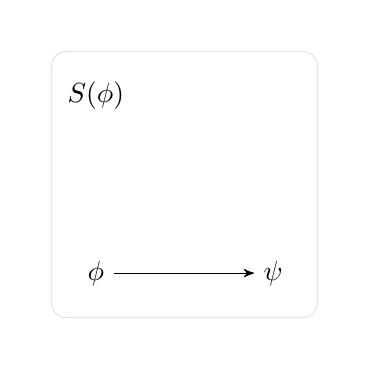
\begin{tikzpicture}[->, >=stealth', node distance=0cm, every text node part/.style={align=center}, scale=0.75]
        \node [] (1) at (-1,4) {};
        \node [] (2) at (-1,-1) {};
        \node [] (3) at (4,-1) {};
        \node [] (4) at (4,4) {};

        \node [] (a) at (0,3) {\(S(\phi)\)};
        \node [] (b) at (0,0) {\(\phi\)};
        \node [] (c) at (3,0) {\(\psi\)};
        \node [] (d) at (3,3) {};

        \draw [->, xshift=4] (b) to  node[right] {} (c);
        \draw [rounded corners=5pt, opacity=.1] (-.75,3.75) -- (-.75,-.75) -- (3.75,-.75) -- (3.75,3.75) -- cycle;
      \end{tikzpicture}
      \caption{Support for \(S(\phi)\) and info}
    \end{subfigure}
    \hfill
    \begin{subfigure}{.45\textwidth}
      \centering
      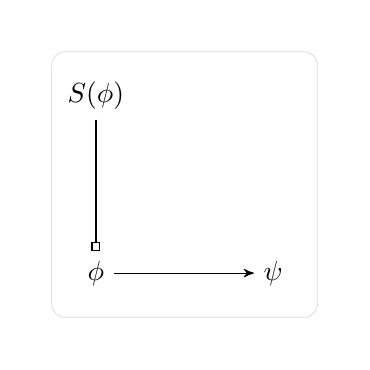
\begin{tikzpicture}[->, >=stealth', node distance=0cm, every text node part/.style={align=center}, scale=0.75]
        \node [] (1) at (-1,4) {};
        \node [] (2) at (-1,-1) {};
        \node [] (3) at (4,-1) {};
        \node [] (4) at (4,4) {};

        \node [] (a) at (0,3) {\(S(\phi)\)};
        \node [] (b) at (0,0) {\(\phi\)};
        \node [] (c) at (3,0) {\(\psi\)};
        \node [] (d) at (3,3) {};

        \draw [->] (b) to  node[right] {} (c);
        \draw [->, -{Square[open]}] (a) to  node[right] {} (b);
        \draw [rounded corners=5pt, opacity=.1] (-.75,3.75) -- (-.75,-.75) -- (3.75,-.75) -- (3.75,3.75) -- cycle;
      \end{tikzpicture}
      \caption{Move to value of \(\phi\)}
    \end{subfigure}

    \begin{subfigure}{.45\textwidth}
      \centering
      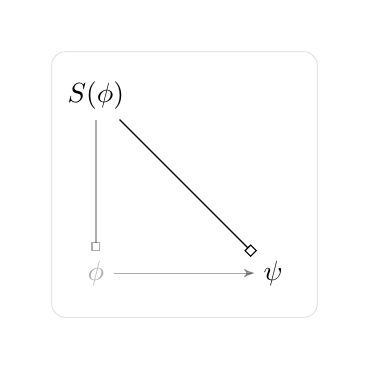
\begin{tikzpicture}[>=stealth', node distance=0cm, every text node part/.style={align=center}, scale=0.75]
        \node [] (1) at (-1,4) {};
        \node [] (2) at (-1,-1) {};
        \node [] (3) at (4,-1) {};
        \node [] (4) at (4,4) {};

        \node [] (a) at (0,3) {\(S(\phi)\)};
        \node [opacity=0.33] (b) at (0,0) {\(\phi\)};
        \node [] (c) at (3,0) {\(\psi\)};
        \node [] (d) at (3,3) {};

        \draw [->, opacity=0.33] (b) to  node[right] {} (c);
        \draw [->,-{Square[open]}, opacity=0.33] (a) to  node[right] {} (b);
        \draw [->,-{Square[open]}] (a) to  node[right] {} (c);
        \draw [rounded corners=5pt, opacity=.1] (-.75,3.75) -- (-.75,-.75) -- (3.75,-.75) -- (3.75,3.75) -- cycle;
      \end{tikzpicture}
      \caption{Given support, value of \(\psi\) is determined}
    \end{subfigure}
    \hfill
    \begin{subfigure}{.45\textwidth}
      \centering
      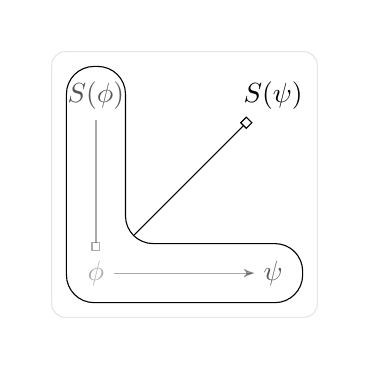
\begin{tikzpicture}[>=stealth', node distance=0cm, every text node part/.style={align=center}, scale=0.75]
        \node [] (1) at (-1,4) {};
        \node [] (2) at (-1,-1) {};
        \node [] (3) at (4,-1) {};
        \node [] (4) at (4,4) {};

        \node [opacity=0.66] (a) at (0,3) {\(S(\phi)\)};
        \node [opacity=0.33] (b) at (0,0) {\(\phi\)};
        \node [opacity=0.66] (c) at (3,0) {\(\psi\)};
        \node [] (d) at (3,3) {\(S(\psi)\)};

        \draw [->, opacity=0.33] (b) to  node[right] {} (c);
        \draw [->,-{Square[open]}, opacity=0.33] (a) to  node[right] {} (b);

        \draw [rounded corners=10pt] (-.5,3.5) -- (-.5,-.5) -- (3.5,-.5) -- (3.5,.5) -- (.5,.5) -- (.5,3.5) -- cycle;
        \draw [->,-{Square[open]}] (.64,.64) to node[right] {} (d);

        \draw [rounded corners=5pt, opacity=.1] (-.75,3.75) -- (-.75,-.75) -- (3.75,-.75) -- (3.75,3.75) -- cycle;
      \end{tikzpicture}
      \caption{Support for \(\psi\) from constraint on \(\psi\) following from support for \(\phi\)}
    \end{subfigure}
    \caption{\RBV{} diagram}
  \end{figure}
\end{note}


\begin{note}[Non-\RBV{} reasoning]
  Not all reasoning is like this.

  Return to examples used to illustrate inclusion of support.
  \begin{itemize}
  \item Conjunction elimination.
    Here, working with the logical form, it doesn't matter what \(p\), \(q\), nor \(r\) are.
  \item Same for efficient route example.
    Agent doesn't need to appeal to having found the most efficient route to produce variation.
  \end{itemize}

  Some instance of reasoning may go either way.
  For example.
  Machine.
  Told that the machine is designed to perform some function, but not told what the function is.

  Question, \(f(X,Y)\)

  One option is to input into machine.
  So, relying on machine implementing function.
  Going by value.

  Second option, abstract function from machine by inspection.
  Then, calculate \(f(X,Y)\).
  Not going by value, doesn't matter what the machine produced.

  Risks for each.
  For the first, potential malfunction on specific input, but without malfunction then that's the result.
  For the second, no concern about potential malfunction, but possible that abstracted function is faulty.

  So, difference is not tied to proposition.

  And, complex chain of reasoning may include both.
  \(p \rightarrow (q \land K_{S}r)\) so \(p \rightarrow q \land r\).
\end{note}


\section{Difficult Cases}
\label{sec:difficult-cases}


\begin{note}[General form of difficult cases]
  Generate difficult cases in a systematic way.
  Roughly, any time someone implements something that is a shortcut to other information.
  Return to calculator illustration.
  Something puzzling about the technician.
  However, this is quite common.

  Bookmark.
  Easy to check that this is how far I've got in the book.
  If not, then the bookmark is no good.

  Doorbell, but in a position to check whether there is someone at the door.

  Requests for a colleague to perform some task.
  I.e.\ spreadsheets.

  The key point with all of these examples is that the shortcut is only good if you think that the relevant \(\psi\) instance is the case.
  So, breaks the `\eit{}'.

  However, this goes to fast.
  What we're picking up is not that \(\psi\) needs to be the case --- that much is clear from \ref{nI:claimed-support} --- but that the agent is in a position to claim support for \(\psi\) without appeal to value of \(\phi\).
  The issue is not that \(\psi\) is required to be the case, such a result is the use of reasoning by value.
  No, the issue is with whether the claimed support for \(\phi\) really is any good.

  Hence, the problem highlighted here is roughly that things need to function as expected in order for shortcuts to be of any use.
  Still, there is a difference between \(\phi\) and \(\psi\) working together for the shortcut, and appealing to \(\phi\) and the shortcut requiring \(\psi\) to observe that \(\psi\) is the case and hence you were fine to appeal to the shortcut.

  The latter is intuitively problematic.
  Lots of things going on.
  Here, suggestion is that at least one, sufficient for failure, is that we've got no idea whether the shortcut works.
  It might, but we're appealing to success in order to argue that it does.
  This is what is repeated and expanded on.
  Issue is not that \(\psi\) is required by \(\phi\).
  Rather, that \(\psi\) is required in order to the agent to appeal to claimed support.
  Observing that \(\psi\) follows is then of no real interest, because if not \(\psi\) then no idea about \(\phi\).

  This doesn't fully resolve the query, though.
  We've shown that shortcuts are plausibly OK when \ref{nI:inclusion} doesn't hold.
  However, many cases in which it does seem to hold, and the shortcut seems to be fine.
  The shortcut is there because it's reduces effort.
  And, with a little more effort, one could check the \(\psi\) condition.

  Easy to deal with in the case of testimony.
  Conditional is truthful then something mundane.
  Here, if the \(\psi\) condition doesn't hold, then it's really not clear that one gets a problem with the claimed support for testimony.
  The issue is very local, and claim for testimony would need to be unreasonably strong.
  And, conversely, does seem problematic if the testimony claim is extremely narrow.
  So, the point is that there's no plausible instance of \ref{nI:inclusion} for testimony case, even though the \(\psi\) condition is true.

  So, \nI{} applies to these one-off cases, or when there is going to be some significant problem from a single point of failure.

  Still, the problem identified by \nI{} differs slightly.
  Latter is intuitively problematic because using the result of an assumption to discharge the use of the assumption.
  \nI{} doesn't require assuming claimed support for \(\psi\).
  Rather, 

  Corollary is that one needs to expand as much as possible when one can.
  Commendable, but does not seem required for claiming support.
\end{note}


\section{Deviousness}
\label{sec:deviousness}

\begin{note}
  Consider Wally example.
  It seems as though there's no way to string together some alternative route when reasoning by value to claim support that the individual is wearing round glasses.
  That is, I may not add in any intermediate steps that go beyond what I am in a position to claim support for (independent of the individual being Wally).

  This is on the one hand expected, and on the other hand surprising.

  However, it's not so simple.
  For example, you and I identified the same individual, and by the way did you notice the round glasses.
  Here, I've got testimony that the individual is wearing glasses.
  And, it doesn't seem as though I need to check testimony.
  This of course depends on one's view of testimony.
  Plausibly, however, it's fine.
  So, the above isn't quite true.
  At least, not without additional clauses.
\end{note}

\chapter{Tension}
\label{cha:tension}

\subsection{Overview of argument for tension}
\label{sec:overv-argum-tens}

\begin{note}[Conflict with the other two principles]
  The two different ways of understanding ability lead to conflict with the two other principles.
\end{note}

\begin{note}[Witnessing]
  The conflict between \ref{denied-claim} and witnessing is straightforward.

  For,~\ref{denied-claim} denies the possibility of witnessing in any case of ability.
  As the agent has not performed the reasoning, the agent is not in a position to appeal to the premises.
\end{note}

\begin{note}[Attribution]
  The conflict between~\nI{} and attribution requires the assumption from~\ref{prem:ab}.

  For, then the agent is appealing to the `leadingness' of their support for the general ability.
\end{note}

\begin{note}[Result from tension]
  So long as there's tension, this is a useful result, I think.
\end{note}

\begin{note}[Preferred resolution]
  Defend both~\nI{} and~\ref{prem:ab}.
  Therefore, not~\ref{denied-claim}.

  Given that both~\ref{denied-claim} and~\nI{} are quite intuitive, deny~\ref{prem:ab}.

  Sketched a straightforward argument from~\ref{denied-claim} to denying witnessing.
  Further, there are some subtleties with \nI{} and \ref{prem:ab} independent of \ref{denied-claim}.

  Picture on which there are exceptions to~\ref{denied-claim} so long as the agent is able to appeal to premises that they would trace support from in the relevant witnessing event of ability.

  Two lines of argument for denying~\ref{denied-claim}.
  \begin{enumerate}
  \item We have a motivated restriction on~\ref{prem:ability}.
  \item Witnessing provides an intuitive understanding of cases in which agent has the option of appealing to ability.
  \end{enumerate}
  These two lines of argument work together.
  The tension generates interest in witnessing that may be flatly rejected by prior endorsement of~\ref{denied-claim}.
  The intuitive understanding of scenarios involving ability suggests there's more to witnessing than resolving the tension in narrow cases.

  To help situate, begin by sketching restriction on~\ref{denied-claim}.
\end{note}

\subsection{A little more detail}
\label{sec:little-more-detail}

The argument is by counter-example.
Rejection of~\ref{denied-claim} is somewhat narrow.

\begin{enumerate}[]
\item\label{access} If premises imply conclusion, then if agent accesses support they have for premises and traces implication through reasoning, then agent obtains support for conclusion on basis of support for premises
\end{enumerate}

Basic.
Understanding of implication is put in the background.
May understand this as something quite trivial.

\begin{enumerate}[]
\item\label{access:exception} If agent is able to obtain support for conclusion on basis of support for premises by accesses support they have for premises and reasoning to conclusion, then if agent accesses support they have for premises and traces implication through reasoning, then agent obtains support for conclusion on basis of support for premises.
\end{enumerate}

If agent may do something to achieve a result, then they would achieve the result by doing the thing.
Embedded conditional captures a witnessing event of the ability.

Agent is required to witness the ability, if the agent is appealing to witnessing.

Compatible with the agent reasoning from their ability.

This is where the tension comes.
Scenarios in which it is permissible for agent to appeal to reasoning they are able to do in order to support a conclusion.

This narrows significantly.

Still, the type of counterexample is further constrained.
Here, the argument splits.

First, the counterexample with \nI{}.
Second, the upshots of denying~\ref{denied-claim}.

Counterexample requires alternative in some cases of ability, and given alternative is required, it expands to other cases of ability.

Remains a somewhat narrow exception to~\ref{denied-claim}.



\subsection{Denying ability}
\label{sec:denying-ability}

\begin{note}[Difficult corollary of argument]
Given that both~\ref{denied-claim} and~\nI{} are quite intuitive, deny~\ref{prem:ab}.
Strengthen the argument by observing a corollary.

\begin{enumerate}
\item\label{prem:ab:cor:a} The agent appeals to a potential witnessing event of an ability that the agent has in order to obtain support for some proposition without having appropriate support for the ability to generate the witnessing event.
\end{enumerate}

This is why~\ref{prem:ab} is phrased in terms of information, rather than support.

\nI{} does not prevent the agent from using the proposition.
\ref{prem:ab} only denies that the agent obtains support.

By appealing to witness, the agent isn't appealing to support.

So, in certain situations, propositions on the basis of such information may still be used.

Key idea here is that the agent doesn't have support either way.
And, it's the application of the general ability (which the agent does have support for) which does the work.

Corollary~\ref{prem:ab:cor:a} and an exception to~\ref{denied-claim} when dealing with ability is preferable to an exception to~\nI{}.
\end{note}

\begin{note}[Second aspect of corollary]
  Generalise~\ref{prem:ab:cor:a}:
  \begin{enumerate}
  \item\label{prem:ab:cor:b} Use a proposition \(\phi\) to obtain support for some other proposition \(\psi\) without support for \(\phi\).
  \end{enumerate}
  However, there are various instances where this seems fine.
  There's Wright, at least.
\end{note}

\begin{note}[Narrowing understanding of support]
A second option is to deny that the agent obtains support.
If so, no tension.
Quite plausible, at least on some ways of understanding support.

However, then left with a variant of support for which~\ref{denied-claim} does not hold.
The main focus on~\ref{denied-claim} is not support, but the accessibility requirement.
Our use of `support' is something of a generic placeholder.
\end{note}

\begin{note}[Too narrow]
  Hold that the exception made by~\ref{prem:ab} is too narrow to be of general interest.
  Supplemental argument that witnessing offers natural interpretation, even when there's the option of attribution.

  (And possibly that attribution seems to over-generate support.)
\end{note}

\begin{note}[More on too narrow]
  Idealised agents have no need for abilities.
However, for non-ideal agents, abilities seems useful.
Information about ability may be abundant while the resources for witnessing abilities are either scarce or temporarily unavailable.
So, agent is able to conserve or defer use of resources.
\end{note}


\subsection{Strength of \ESU{}}
\label{sec:appeal-main-premise}

Denying the \ESU{} is difficult.
The general principle provides a recipe for dealing with every other case.
However, given that the agent does some reasoning, seems there's always the option to identify the reasoning done with the reasons the agent appeals to.
So, given that there's always something for the \ESU{} to use, it seems that in the absence of any serious difficulty with the \ESU{}, alternatives lose out.

Further, simple failure of \ESU{} isn't particularly informative.
Seems good in many cases.
And, rules out many bad cases.
If the \ESU{} fails in general, then an account of why.

The strategy is split into two parts:
\begin{enumerate}
\item Identify a kind of case where the assumption is problematic, motivating an exception to the general principle.
\item Argue that if the exception is granted, then there are further cases of similar kind in which the alternative is compelling, even if the general principle holds.
\end{enumerate}

The strategy is straightforward.
Identifying a kind of counterexample means that one is not in a position to apply the general principle universally.
Given counterexample, then we have an alternative account for at least one kind of case.
Consider other cases in which the alternative may apply.
It is not the case that we don't have an argument for accessibility based on the application of a general principle.
Suggest that the alternative fares well in the absence of a general principle.

Then, so long as the structure in place for the alternative is fairly common, there is potential to re-evaluate arguments that involve the general principle.


\begin{note}[Denying \nI{} and \WR{}, a bullet to bite?]
  It looks as though I end up with:

  The agent appeals to a potential witnessing event of an ability that the agent has in order to obtain support for some proposition without having appropriate support for the ability to generate the witnessing event.

  Well, the ability is not the thing providing the support.
  So, lacking support for the ability is not the issue.

  The question is about why the agent is in a position to appeal to those reasons.

  Well, there's an additional constraint, possibly.
  Roughly, it is impermissible for an agent to hold a contrary attitude to a proposition that they're committed to.

  Well, then the agent does not have support for possessing the ability.

  This is somewhat disconcerting, but not particularly problematic.

  The key observation is that \nI{} means that the agent does not obtain support.
  This does not mean that the agent does not have the option of using the information.
\end{note}

\hozline{}

Problematic cases, are, roughly put, useful for understanding how things are.

Still, because particular case, then the rejection of~\ref{denied-claim} is limited.
I think the core of~\ref{denied-claim} often holds.
The concern is that~\ref{denied-claim} applies to all instances of reasoning.

Interest is in the role of~\ref{denied-claim} in arguments and understanding phenomena.
If there are exceptions to~\ref{denied-claim}, then if~\ref{denied-claim} is a premise, there may be variants on the relevant conclusion, and if~\ref{denied-claim} is a conclusion, then potential issues with premises, or links between them.




Well, this is the strong way of putting the argument.
The slightly weaker version is to hold that there is not a sense of support which holds for both reasoning and the use of abilities.

In this sense, the notion of support captured by~\ref{denied-claim} is not the only notion of support of interest.

Familiar with assuming and so on.
Key difference here is that the agent appeals to support.

Before continuing, narrow down.



\section{Ability}
\label{sec:ability}

First explain how ability relates, and how it suggests an alternative.

\subsection{Why ability is interesting}
\label{sec:why-abil-inter}

\begin{enumerate}
\item Reasoning is an action, a particular event.
\item Ability grants a potential witnessing event.
\end{enumerate}

Reasoning is some event, and ability allows us to attribute the agent the potential to witness the relevant event.

Certain kinds of ability.

The interest here is that we have a clear understanding of how reasoning works, related to the general premise.
With ability to reason, there are two things:
\begin{enumerate}
\item The reasoning which the agent may witness.
\item Having the ability to generate the witnessing event.
\end{enumerate}

By the general premise, it seems that if the agent were to witness the reasoning, then those things appealed to in reasoning would support the premise.
However, as the agent has not yet reasoned, having the ability should do the work.

So, this is the suggested alternative.
In some cases, witnessing.

If witnessing, then the conflict with the general principle is that as the agent has not done the reasoning, the agent doesn't have access to those reasons.
However, the reasons are there for the agent.

Two things about why ability is interesting.

Understand that if the agent has the ability, then they may witness reasoning.
However, ability secures only the potential.
Not in the sense that the there is a potential for a coin flip to land heads, but in that a coin with heads on both sides has the potential to land heads up when flipped --- the coin merely needs to be flipped.

Things follow from witnessing abilities.
Factive verbs work best here.
Key is that the relevant proposition is true whether or not the agent witnesses the ability.
Some propositions are only true after witnessing.

Simple example is \(\phi\), and `that I have \emph{V}'d that \(\psi\)'.
\(\phi\) must be true in order for the agent to \emph{V} that \(\phi\).
Still, `that I have \emph{V}'d that \(\psi\)' is only true when the agent has \emph{V}'d that \(\phi\).

Two different ways of understanding ability provide different perspectives.

If the agent reasons, then the agent obtains support for \(\phi\) which do not necessarily depend on a premise that the agent has the ability.
Easy to see with logic examples.
The agent witnesses the ability, but in so exercising does not need to appeal to the observation that they are witnessing.
Many cases where recognition of ability is only after witnessing it.

If the agent appeals to the attribute, then ability is a key premise.
The agent obtains \(\phi\) because if \(\phi\) were not the case, the agent wouldn't have the ability to \emph{V} that \(\phi\).

So, in principle there's two ways in which ability may be put to work.

One further complication.
Agent may not need to put ability to work.

Possible for agent to be provided with support for \(\phi\) and support for the ability to \emph{V} that \(\phi\).
For example, testimony, say.
Distinct from \(A(\phi)\) therefore \(\phi\) must be the case.

If so, ability is not of interest in obtaining a conclusion.

\begin{enumerate}
\item\label{cases-of-i-ex} There are cases in which \(A(\phi)\) is required for \(\phi\).
\end{enumerate}

\ref{cases-of-i-ex} holds that there are cases in which the agent has information that \(A(\phi)\), understands that \(A(\phi) \rightarrow \phi\), and has no other way of obtaining \(\phi\) other than by \(A(\phi)\).

\subsection{Ability used in basing relation}
\label{sec:ability-used-basing}

\cite{Leite:2004uv} more-or-less defines basing relation in terms of ability.
So, expands on a consequence of this.
%%% Local Variables:
%%% mode: latex
%%% TeX-master: "master"
%%% End:


\part{Positive argument}

\part{Temporary}

%%% Local Variables:
%%% TeX-master: "AbilityMaster"
%%% End:%%% Local Variables:
%%% TeX-master: "master"
%%% End:

\chapter{Notes}
\label{cha:notes}

\section{Names}
\label{sec:names}

\begin{itemize}
\item[(uRp)] Use requires possession.
\item[(uRh)] Use requires having.
\item[(uRa)] \mp{-}.\newline
  うら (裏)
\end{itemize}



\subsection{Motivation for \mp{}}
\label{sec:motiv-main-prem}

Some motivation for the \mp{}:

\begin{enumerate}
\item Davidson
\item Responding to reasons
\item Hieronymi
\item Intuitive
\end{enumerate}

Broadly, the \mp{} is interesting because it constrains how an agent obtains some conclusion by reasoning.
Instances that conform seem good, and instances that do not conform seem bad.

[Examples]

May also see how this is applied when finding solutions to difficult cases.
For example, the \mp{} is in the background with Bratman on temptation, where the central idea is that desires fail to count as reasons because the agent would then need to act in a certain way.

\printbibliography

\end{document}
